% Options for packages loaded elsewhere
\PassOptionsToPackage{unicode}{hyperref}
\PassOptionsToPackage{hyphens}{url}
%
\documentclass[
  donotrepeattitle,doc, 12pt, a4paper,floatsintext]{apa7}
\usepackage{amsmath,amssymb}
\usepackage{lmodern}
\usepackage{iftex}
\ifPDFTeX
  \usepackage[T1]{fontenc}
  \usepackage[utf8]{inputenc}
  \usepackage{textcomp} % provide euro and other symbols
\else % if luatex or xetex
  \usepackage{unicode-math}
  \defaultfontfeatures{Scale=MatchLowercase}
  \defaultfontfeatures[\rmfamily]{Ligatures=TeX,Scale=1}
  \setmainfont[]{Times New Roman}
\fi
% Use upquote if available, for straight quotes in verbatim environments
\IfFileExists{upquote.sty}{\usepackage{upquote}}{}
\IfFileExists{microtype.sty}{% use microtype if available
  \usepackage[]{microtype}
  \UseMicrotypeSet[protrusion]{basicmath} % disable protrusion for tt fonts
}{}
\makeatletter
\@ifundefined{KOMAClassName}{% if non-KOMA class
  \IfFileExists{parskip.sty}{%
    \usepackage{parskip}
  }{% else
    \setlength{\parindent}{0pt}
    \setlength{\parskip}{6pt plus 2pt minus 1pt}}
}{% if KOMA class
  \KOMAoptions{parskip=half}}
\makeatother
\usepackage{xcolor}
\usepackage{graphicx}
\makeatletter
\def\maxwidth{\ifdim\Gin@nat@width>\linewidth\linewidth\else\Gin@nat@width\fi}
\def\maxheight{\ifdim\Gin@nat@height>\textheight\textheight\else\Gin@nat@height\fi}
\makeatother
% Scale images if necessary, so that they will not overflow the page
% margins by default, and it is still possible to overwrite the defaults
% using explicit options in \includegraphics[width, height, ...]{}
\setkeys{Gin}{width=\maxwidth,height=\maxheight,keepaspectratio}
% Set default figure placement to htbp
\makeatletter
\def\fps@figure{htbp}
\makeatother
\setlength{\emergencystretch}{3em} % prevent overfull lines
\providecommand{\tightlist}{%
  \setlength{\itemsep}{0pt}\setlength{\parskip}{0pt}}
\setcounter{secnumdepth}{5}
% Make \paragraph and \subparagraph free-standing
\ifx\paragraph\undefined\else
  \let\oldparagraph\paragraph
  \renewcommand{\paragraph}[1]{\oldparagraph{#1}\mbox{}}
\fi
\ifx\subparagraph\undefined\else
  \let\oldsubparagraph\subparagraph
  \renewcommand{\subparagraph}[1]{\oldsubparagraph{#1}\mbox{}}
\fi
\newlength{\cslhangindent}
\setlength{\cslhangindent}{1.5em}
\newlength{\csllabelwidth}
\setlength{\csllabelwidth}{3em}
\newlength{\cslentryspacingunit} % times entry-spacing
\setlength{\cslentryspacingunit}{\parskip}
\newenvironment{CSLReferences}[2] % #1 hanging-ident, #2 entry spacing
 {% don't indent paragraphs
  \setlength{\parindent}{0pt}
  % turn on hanging indent if param 1 is 1
  \ifodd #1
  \let\oldpar\par
  \def\par{\hangindent=\cslhangindent\oldpar}
  \fi
  % set entry spacing
  \setlength{\parskip}{#2\cslentryspacingunit}
 }%
 {}
\usepackage{calc}
\newcommand{\CSLBlock}[1]{#1\hfill\break}
\newcommand{\CSLLeftMargin}[1]{\parbox[t]{\csllabelwidth}{#1}}
\newcommand{\CSLRightInline}[1]{\parbox[t]{\linewidth - \csllabelwidth}{#1}\break}
\newcommand{\CSLIndent}[1]{\hspace{\cslhangindent}#1}
\ifLuaTeX
\usepackage[bidi=basic]{babel}
\else
\usepackage[bidi=default]{babel}
\fi
\babelprovide[main,import]{english}
% get rid of language-specific shorthands (see #6817):
\let\LanguageShortHands\languageshorthands
\def\languageshorthands#1{}
% Manuscript styling
\usepackage{upgreek}
\captionsetup{font=singlespacing,justification=justified}

% Table formatting
\usepackage{longtable}
\usepackage{lscape}
% \usepackage[counterclockwise]{rotating}   % Landscape page setup for large tables
\usepackage{multirow}		% Table styling
\usepackage{tabularx}		% Control Column width
\usepackage[flushleft]{threeparttable}	% Allows for three part tables with a specified notes section
\usepackage{threeparttablex}            % Lets threeparttable work with longtable

% Create new environments so endfloat can handle them
% \newenvironment{ltable}
%   {\begin{landscape}\centering\begin{threeparttable}}
%   {\end{threeparttable}\end{landscape}}
\newenvironment{lltable}{\begin{landscape}\centering\begin{ThreePartTable}}{\end{ThreePartTable}\end{landscape}}

% Enables adjusting longtable caption width to table width
% Solution found at http://golatex.de/longtable-mit-caption-so-breit-wie-die-tabelle-t15767.html
\makeatletter
\newcommand\LastLTentrywidth{1em}
\newlength\longtablewidth
\setlength{\longtablewidth}{1in}
\newcommand{\getlongtablewidth}{\begingroup \ifcsname LT@\roman{LT@tables}\endcsname \global\longtablewidth=0pt \renewcommand{\LT@entry}[2]{\global\advance\longtablewidth by ##2\relax\gdef\LastLTentrywidth{##2}}\@nameuse{LT@\roman{LT@tables}} \fi \endgroup}

% \setlength{\parindent}{0.5in}
% \setlength{\parskip}{0pt plus 0pt minus 0pt}

% Overwrite redefinition of paragraph and subparagraph by the default LaTeX template
% See https://github.com/crsh/papaja/issues/292
\makeatletter
\renewcommand{\paragraph}{\@startsection{paragraph}{4}{\parindent}%
  {0\baselineskip \@plus 0.2ex \@minus 0.2ex}%
  {-1em}%
  {\normalfont\normalsize\bfseries\itshape\typesectitle}}

\renewcommand{\subparagraph}[1]{\@startsection{subparagraph}{5}{1em}%
  {0\baselineskip \@plus 0.2ex \@minus 0.2ex}%
  {-\z@\relax}%
  {\normalfont\normalsize\itshape\hspace{\parindent}{#1}\textit{\addperi}}{\relax}}
\makeatother

% \usepackage{etoolbox}
\makeatletter
\patchcmd{\HyOrg@maketitle}
  {\section{\normalfont\normalsize\abstractname}}
  {\section*{\normalfont\normalsize\abstractname}}
  {}{\typeout{Failed to patch abstract.}}
\patchcmd{\HyOrg@maketitle}
  {\section{\protect\normalfont{\@title}}}
  {\section*{\protect\normalfont{\@title}}}
  {}{\typeout{Failed to patch title.}}
\makeatother

\usepackage{xpatch}
\makeatletter
\xapptocmd\appendix
  {\xapptocmd\section
    {\addcontentsline{toc}{section}{\appendixname\ifoneappendix\else~\theappendix\fi\\: #1}}
    {}{\InnerPatchFailed}%
  }
{}{\PatchFailed}
\keywords{keywords\newline\indent Word count: 2004}
\usepackage{csquotes}
\usepackage[titles]{tocloft}
\cftpagenumbersoff{figure}
\renewcommand{\cftfigpresnum}{\itshape\figurename\enspace}
\renewcommand{\cftfigaftersnum}{.\space}
\setlength{\cftfigindent}{0pt}
\setlength{\cftafterloftitleskip}{0pt}
\settowidth{\cftfignumwidth}{Figure 10.\qquad}
\cftpagenumbersoff{table}
\renewcommand{\cfttabpresnum}{\itshape\tablename\enspace}
\renewcommand{\cfttabaftersnum}{.\space}
\setlength{\cfttabindent}{0pt}
\setlength{\cftafterloftitleskip}{0pt}
\settowidth{\cfttabnumwidth}{Table 10.\qquad}
\pagestyle{plain}
\usepackage{adjustbox}
\setcounter{tocdepth}{5}
\linespread{1.2}
\usepackage{setspace}
\shorttitle{}
\rhead{DoPL and DOSPERT}
\usepackage{fancyhdr}
\cfoot{\thepage}
\fancyheadoffset[L]{0pt}
\fancyhf{}
\fancyhead[RO,LE]{\small\thepage}
\renewcommand{\headrulewidth}{0pt}
\interfootnotelinepenalty=10000
\newcommand{\HRule}{\rule{\linewidth}{0.25mm}}
\let\cleardoublepage=\clearpage
\doublespacing
\usepackage{pdflscape}
\ifLuaTeX
  \usepackage{selnolig}  % disable illegal ligatures
\fi
\IfFileExists{bookmark.sty}{\usepackage{bookmark}}{\usepackage{hyperref}}
\IfFileExists{xurl.sty}{\usepackage{xurl}}{} % add URL line breaks if available
\urlstyle{same} % disable monospaced font for URLs
\hypersetup{
  pdftitle={The psychology of risk and power: Power desires and sexual choices.},
  pdfauthor={Ithurburn, Andrew1},
  pdflang={en-EN},
  pdfkeywords={keywords},
  hidelinks,
  pdfcreator={LaTeX via pandoc}}

\title{The psychology of risk and power: Power desires and sexual choices.}
\author{Ithurburn, Andrew\textsuperscript{1}}
\date{}


\shorttitle{RISK AND POWER}

\authornote{

Add complete departmental affiliations for each author here. Each new line herein must be indented, like this line.

Enter author note here.

The authors made the following contributions. Ithurburn, Andrew: .

Correspondence concerning this article should be addressed to Ithurburn, Andrew, 7 George Square, Edinburgh, EH8 9JZ. E-mail: \href{mailto:a.ithurburn@sms.ed.ac.uk}{\nolinkurl{a.ithurburn@sms.ed.ac.uk}}

}

\affiliation{\vspace{0.5cm}\textsuperscript{1} The University of Edinburgh}

\abstract{%
One or two sentences providing a \textbf{basic introduction} to the field, comprehensible to a scientist in any discipline.

Two to three sentences of \textbf{more detailed background}, comprehensible to scientists in related disciplines.
}



\begin{document}
\maketitle

\clearpage

\mbox{}\thispagestyle{empty}\clearpage
\setcounter{page}{1}
\thispagestyle{empty}

\begin{center}
\vspace*{10mm}
\rule{\linewidth}{0.25mm}\\
\textbf{\Large The psychology of risk and power: Power desires and sexual choices}\\
\rule{\linewidth}{0.25mm}\\
\vspace*{10mm}
\textbf{Andrew Ithurburn}\\
\begin{figure}[ht]
\begin{center}
\includegraphics[width=!,totalheight=!,scale=0.25]{../Formatting/EdUniCrest.jpg}
\end{center}
\end{figure}
{\setstretch{1.7} 
Doctor of Philosophy\\
\smallskip
\smallskip
THE UNIVERSITY OF EDINBURGH\\
\smallskip
}
\end{center}
\clearpage

\mbox{}\thispagestyle{empty}\clearpage

\newpage

\tableofcontents

\newpage

\hypertarget{literature-review}{%
\section{Literature Review}\label{literature-review}}

\hypertarget{general-introduction}{%
\subsection{General Introduction}\label{general-introduction}}

In 2016, the year of most recent global data collection, there were 376 million new cases of the four curable sexually transmitted infections, chlamydia, gonorrhea trichomoniasis, and syphilis (\protect\hyperlink{ref-worldhealthorganization2018}{Organization, 2018}). The World Health Organization (WHO) further estimates that there are one million new cases of a curable sexually transmitted infection each day. Due to multiple factors, certain minoritpopulations are more at risk for contracting new sexually transmitted infections, e., men who have sex with men and female sex workers (\protect\hyperlink{ref-worldhealthorganization2018}{Organization, 2018}). Some factors includcertain societal beliefs men who have sex with men might engage in nonrelational sex ``just trying to figure things out it's just a hook-up phase'' (\protect\hyperlink{ref-elder2015a}{Elder et al., 2015}), ambiguous laws concerning the legality of sex work interfering with safe and available locations for such activity, as well. Often, societal beliefs impact discussions of sexual exploration making sexual explorations in themselves difficult and taboo (\protect\hyperlink{ref-parent2015}{Parent et al., 2015}). There may also be some difficulties in their willingness in their activities be it forced by another or sheer necessity. For countries like Scotland while there has been a reduction in the number of new cases of STIs like HIV amongst key populations, new risks of antibiotic-resistant gonorrhea, \emph{Neisseria gonorrhoaeae}, have become more apparent (\protect\hyperlink{ref-ison2011}{Ison \& Alexander, 2011}).

Outside of the Scotland, such as England, STI rates still show relatively high numbers with new cases nymber in 317,000 cases (\protect\hyperlink{ref-ratna2021}{Ratna et al., 2021}). Optimistically, STI rates have reduced in the last year before publication of the report by nearly 34\%. However, it should be noted that there was a 25\% decrease in the number of sexual health screenings compared to the previous year which the authors note as contributing to the decrease in STI diagnoses (\protect\hyperlink{ref-ratna2021}{Ratna et al., 2021, p. 5}). Furthering, outside of the United Kingdom, global STI rates are still increasingly especially in areas with little to know access to appropriate sexual health education and health care to support the increasing number. According to the World Health Organization, 1 million people are infected with an STI each day (\protect\hyperlink{ref-worldhealthorganization2022}{World Health Organization, 2022}). Including an estimated annual death toll of 2.3 million people. Along with death, STI infection can leads to financial, social, and psychological issues and trauma (\protect\hyperlink{ref-deal2004}{Deal et al., 2004}; \protect\hyperlink{ref-delva1983}{Delva, 1983}; \protect\hyperlink{ref-henkel2004}{Henkel, 2004}; \protect\hyperlink{ref-young2007a}{S. D. Young et al., 2007}).

\hypertarget{moral-decision-problems}{%
\subsection{Moral Decision Problems}\label{moral-decision-problems}}

Researching issues such as STIs and other moral laden issues can often be difficult to devise and run. Often, sexually transmitted infections and risky sexual behavior are used as examples to discuss moral issues. Methods at understanding these situations and other moral issues are commonly through dilemmas or vignettes where individuals are presented with a short scenario and asked to choose one outcome over another (\protect\hyperlink{ref-ellemers2019}{Ellemers et al., 2019}). A trademark example is the trolley car experiment where there is a runaway trolley car that is going toward five people (\protect\hyperlink{ref-greene2001}{Greene, 2001}). The decision is thus, to allow the trolley to careen towards the five people or you could divert the trolley by pushing and sacrificing a large man for the sake of the other five. This type of dilemma poses an interesting method of understanding how and what the decision maker would choose. The researcher can then change the dilemma in its severity and complexity. There could also be a change in the situation and the types of individuals that are at risk. Individual choice tasks investigating risky sexual behaviors and STIs could be furthered by investigating the moral decision-making aspect of those issues.

\hypertarget{current-methods-and-problems-in-research}{%
\subsection{Current Methods and Problems in Research}\label{current-methods-and-problems-in-research}}

As such, researching in particular sexually laden moral decisions can often be difficult and complex. Current STI research has focused on methods of ways of curbing individuals act a certain way when presented with a risky sexual situation (\protect\hyperlink{ref-kirby2007}{D. B. Kirby et al., 2007}). Current methods have shown mixed results. In many countries, how people are taught about risk and sex can vary wildly (\protect\hyperlink{ref-unesco2015}{Unesco, 2015}). For example, some countries may have one standard which is a mix of religious and scientific ideas of STIs. While others may not even have a formal sexual education program. Some aspects of sexual activity are not even discussed, for example, non-heterosexual sex (\protect\hyperlink{ref-ellis2004}{Ellis \& High, 2004}). This omission is problematic because historically men who have sex with men in particular, are at a higher risk of contracting an STI (\protect\hyperlink{ref-wald2001}{Wald, 2001}). Often, research can overlook certain aspects of sexual activity and thus will inadvertently miss certain key aspects of researching STIs. Filling that research gap will ultimately benefit our understanding of human behavior and risky behaviors.

\hypertarget{power-and-aggression}{%
\subsection{Power and Aggression}\label{power-and-aggression}}

An interesting outcome of human behavior from moral judgment research and risky decisions is human aggression which is one of the mainstays of power research {[}citation{]}. Aggression, behavior that is committed by the actor to another with the intent to harm the other, is separeated by the reason behind the aggression. For example, if the aggression was intended to be hostile or serve a purpose (hostile aggression and instrumental aggression) (\protect\hyperlink{ref-anderson2002}{C. A. Anderson \& Bushman, 2002}). Looking at human behavior from this perspective allows researchers to look at underlying behavioral characteristics outside of the traditional trauma or action/reaction-based model of human behavior such as behavioral economics.

The me-too movement acted as a watershed moment for often male sexual aggression toward women. Highlighting issues of how these power-over views of women, especially women of color and trans women of color, become learned and develop into sexual aggression. Sexual aggression in and of itself is a subgroup of aggression where the intent to harm is sexual (\protect\hyperlink{ref-anderson2002}{C. A. Anderson \& Bushman, 2002}; \protect\hyperlink{ref-malamuth1995}{Malamuth et al., 1995}). Many of the targets of sexual aggression are women of color and trans women of color (\protect\hyperlink{ref-jefferson2013}{Jefferson et al., 2013} add more citations). In the reported cases men are often the perpetrators of the crimes (\protect\hyperlink{ref-anderson2002}{C. A. Anderson \& Bushman, 2002}). The aggression itself appears to be domain specific to one gender, women. Often, acts of sexual aggression are verbal in nature, such as asking repeatedly for sex or threatening to break up with them (\protect\hyperlink{ref-testa2015}{Testa et al., 2015}). When individuals gain power they may aggress more over those that have less power, which may pay head to the continued sexual aggression and sexual violence against women of color and trans women of color who have historically low levels of power (\protect\hyperlink{ref-jefferson2013}{Jefferson et al., 2013}).

Recent research by Garnett and Mann investigate the cognitive and empathetical processes of those that commit a sexual aggression or sexual violence, labeled as sexual offending (\protect\hyperlink{ref-barnett2013}{2013}). Common to research on sexual offenses, research contends that those that do offend do so with a lack of empathy towards their victims (\protect\hyperlink{ref-marshall1993}{Marshall et al., 1993}). As noted in the previous section on moral judgment, see section 3, empathetic processing by these offenders are more complex than the simple inability to ``feel'' or identify the emotions of others. There is a recurring theme amongst offenders of women being deceitful and sexually entitled (\protect\hyperlink{ref-barnett2013}{Barnett \& Mann, 2013}; \protect\hyperlink{ref-gannon2009}{Gannon, 2009}). The offenders often feel slighted when a woman denies their sexual advances which then tends to lead to some sexual aggression (\protect\hyperlink{ref-gannon2009}{Gannon, 2009}; \protect\hyperlink{ref-williams2017}{Williams et al., 2017}).

The rejection of the sexual advances of the man often damage their sense of masculinity (\protect\hyperlink{ref-malamuth1996}{Malamuth et al., 1996}). Relating back to beliefs on condom use amongst men, even the request of wearing condom could be interpreted as damaging their sense of masculinity (\protect\hyperlink{ref-castrovazquez2000}{Castro-Vázquez, 2000}). If the woman, in a heterosexual relationship, brings the condom they are damaging the males' masculinity but if the male brings the condom he could also be considered a thoughtful individual. While the woman would be seen as easy. This could then lead to bullying behavior and ostracization from the moral judgment of the community on the woman's purity, see section moral judgment.

\hypertarget{chapter-1}{%
\section{Chapter 1:}\label{chapter-1}}

\hypertarget{introduction}{%
\subsection{Introduction}\label{introduction}}

Throughout political history, tyrants, and despots have influenced great power over large swaths of land and communities. One common thread amongst these individuals is how they wield their great power, often through dominant tactics such as threats and political subversion. Recent history has shown with individuals like Donald Trump, Kim Jong-Un, and Rodrigo Duterte who display authoritarian traits often wield their power through fear and threats of violence (\protect\hyperlink{ref-bernstein2020}{Bernstein, 2020}; \protect\hyperlink{ref-bynion2018}{Bynion, 2018}; \protect\hyperlink{ref-kirby2021}{M. Kirby, 2021}). How this power is wielded is often different for each individual. Some individuals such as Duterte and Bolsonaro wielded their power more dramatically than the likes of Trump. Individuals wielding power need not be tyrants such as the former. Individuals like Angela Merkel used her position and leadership skills to be a world leader in most negotiations. While individuals more well known for their status demonstrated their power through prestige motives. To better understand how individuals such as world leaders or opinion makers gain and wield their power over others. Research in this field is often difficult to research yet strides have been made to understand power, namely through research in moral judgment and decision-making such as power orientation.

\hypertarget{dominance-prestige-and-leadership-orientation}{%
\subsection{Dominance, Prestige, and Leadership orientation}\label{dominance-prestige-and-leadership-orientation}}

Research in power desire motives has focused on three subdomains: dominance, leadership, and prestige (\protect\hyperlink{ref-suessenbach2019}{Suessenbach et al., 2019}). Each of these three different power motives is explained as to different ways or methods that individuals in power sought power or were bestowed upon them. Often these dominant individuals will wield their power with force and potentially cause risk to themselves to hold onto that power.

\hypertarget{dominance}{%
\subsubsection{\texorpdfstring{\emph{Dominance}}{Dominance}}\label{dominance}}

The dominance motive is one of the more researched methods and well-depicted power motives. Individuals with a dominant orientation display the more primal human behavior. These individuals will seek power through direct methods such as asserting dominance, control over resources, or physically assaulting someone (\protect\hyperlink{ref-johnson2012}{M. W. Johnson \& Bruner, 2012}; \protect\hyperlink{ref-winter1993}{Winter, 1993}). Early research in dominance motives has shown that acts of dominance ranging from asserting physical dominance over another to physical displays of violence have been shown in many mammalian species, including humans (\protect\hyperlink{ref-petersen2018}{Petersen et al., 2018}; \protect\hyperlink{ref-rosenthal2012}{Rosenthal et al., 2012}).

Individuals high in dominance are often high in Machiavellianism, and narcissism, and often are prone to risky behavior (discussion further in the next section). Continued research has hinted at a possible tendency for males to display these dominant seeking traits more than females (\protect\hyperlink{ref-bareket2020}{Bareket \& Shnabel, 2020}; \protect\hyperlink{ref-sidanius2000}{Sidanius et al., 2000}). When individuals high in dominance assert themselves they are doing so to increase their sense of power (\protect\hyperlink{ref-anderson2012}{C. Anderson et al., 2012}; \protect\hyperlink{ref-bierstedt1950}{Bierstedt, 1950}). Asserting one's sense of dominance over another can be a dangerous task. In the animal kingdom, it can often lead to injury. While, humans asserting dominance can take a multitude of actions such as leering behaviors, physical distance, or other non-verbal methods to display dominance (\protect\hyperlink{ref-petersen2018}{Petersen et al., 2018}; \protect\hyperlink{ref-witkower2020}{Witkower et al., 2020}). Power from a dominant perspective is not always bestowed upon someone. Often, high dominance individuals will take control and hold onto it.

\hypertarget{prestige}{%
\subsubsection{\texorpdfstring{\emph{Prestige}}{Prestige}}\label{prestige}}

Contrary to the dominant motivation of using intimidation and aggression to gain more power, a prestige motivation or prestige, in general, is bestowed upon an individual from others in the community (\protect\hyperlink{ref-maner2016}{Maner \& Case, 2016}; \protect\hyperlink{ref-suessenbach2019}{Suessenbach et al., 2019}). Different from dominance motivation, prestige motivation is generally unique to the human species (\protect\hyperlink{ref-maner2016}{Maner \& Case, 2016}). Due in part to ancestral human groups being smaller hunter-gatherer societies, individuals that displayed and used important behaviors beneficial to the larger group were often valued and admired by the group. Therein, the social group bestows the authority onto the individual. Generally, this type of behavior can be passively achieved by the prestigious individual. However, this does not remove the intent of the actor in that they too can see prestige from the group, but the method of achieving that social status greatly differs from that of dominance-seeking individuals.

Apart from dominance-motivated individuals that continually have to fight for their right to have power over others, individuals that seek or were given power through a prestige motivation are not generally challenged in the same sense as dominant individuals. Displaying behaviors that the community would see as beneficial would endear them to the community making the survival of the community as a whole better (\protect\hyperlink{ref-maner2016}{Maner \& Case, 2016}). Evolutionarily this would increase the viability of the prestigious individual and their genes. Similar to the dominance perspective, the prestige perspective overall increases the power and future survivability of the individual. However, due to the natural difference between prestige and dominance, dominance-seeking individuals are challenged more often resulting in more danger to their position (\protect\hyperlink{ref-johnson2012}{M. W. Johnson \& Bruner, 2012}).

\hypertarget{leadership}{%
\subsubsection{\texorpdfstring{\emph{Leadership}}{Leadership}}\label{leadership}}

With a shared goal a leader is someone that takes initiative and attracts followers for that shared goal (\protect\hyperlink{ref-vanvugt2006}{Van Vugt, 2006}). Leadership is an interesting aspect of behavior in that it is almost exclusive to human interaction. Discussions by evolutionary psychologists point to the formation of early human hunter-gatherer groups where the close interconnectedness created a breeding ground for leadership roles. As early humans began to evolve it would become advantageous for individuals to work together for a common goal (\protect\hyperlink{ref-king2009}{King et al., 2009}). Often, individuals with more knowledge of a given problem would demonstrate leadership and take charge or be given power. Multiple explanations of the evolution of leadership exist such as coordination strategies, and safety, along with evidence for growth in social intelligence in humans (\protect\hyperlink{ref-king2009}{King et al., 2009}; \protect\hyperlink{ref-vanvugt2006}{Van Vugt, 2006}).

An interesting aspect of leadership motivation is the verification of the qualities of the leader by the communities. Individuals that are often put into leadership roles or take a leadership role often display the necessary goals, qualities, and knowledge to accomplish the shared/stated goal. However, this is not always the case, especially for those charismatic leaders who could stay on as a leader longer than the stated goal requires (\protect\hyperlink{ref-vugt2014}{Vugt \& Ronay, 2014}). Traditionally, leadership was thought to be fluid in that those with the necessary knowledge at the time would be judged and appointed as the leader. However, these charismatic leaders use their charisma, uniqueness, nerve, and talent to hold onto their status.

\hypertarget{risk}{%
\subsection{Risk}\label{risk}}

Every time people leave the relative safety of their home, every decision they make they are taking some form of risk. Financial risk is often discussed in the media usually concerning the stock market. However, the risk is not just present in finances but also in social interactions such as social risk, sexual risk, health, and safety risk, recreational, and ethical risks (\protect\hyperlink{ref-breakwell2007}{Breakwell, 2007}; \protect\hyperlink{ref-kuhberger2009}{Kühberger \& Tanner, 2009}; \protect\hyperlink{ref-shearer2005}{Shearer et al., 2005}; \protect\hyperlink{ref-weber2002}{Weber et al., 2002}). Each individual is different in their likelihood and perception of participating in those risks. Some will be more inclined to be more financially risky while others would risk their health and safety.

Whether to engage in a risky situation is very complex depending on a cost-benefit analysis (\protect\hyperlink{ref-johnson2015a}{P. S. Johnson et al., 2015}). Do the positives outweigh the negatives? In practice, not all individuals will do a cost-benefit analysis of a risky situation. Often, the timing of an event makes such an analysis disadvantageous. The benefits are often relative to the individual decision-maker. Differences emerge in the general likelihood to engage in risky behavior such that males tend to be more likely to engage in risky behaviors than their female counterparts (\protect\hyperlink{ref-chen2021}{Chen \& John, 2021}; \protect\hyperlink{ref-desiderato1995}{Desiderato \& Crawford, 1995}). Women tended to avoid risky situations except for social risks.

\hypertarget{experiment-one}{%
\subsection{Experiment One}\label{experiment-one}}

\hypertarget{method}{%
\subsection{Method}\label{method}}

\hypertarget{participants}{%
\subsubsection{Participants}\label{participants}}

Participants were a convenience sample of 95 (Mage = NA, SD = NA) individuals from Prolific Academic crowdsourcing platform (``www.prolific.co''). Requirements for participation were: (1) be 18 years of age or older and (2) and as part of Prolific Academics policy, have a prolific rating of 90 or above. Participants received £4 which amounts to £8 an hour as compensation for completion of the survey. Table 1 demonstrates the demographic information for experiment one.

\begin{table}[tbp]

\begin{center}
\begin{threeparttable}

\caption{\label{tab:unnamed-chunk-9}Participant Demographic Information (Experiment 1)}

\begin{tabular}{ll}
\toprule
Demographic Characteristic & \\
\midrule
Age & \\
\ \ \ Mean (SD) & 26.14 (8.69)\\
\ \ \ Median [Min, Max] & 23 [18,60]\\
Gender & \\
\ \ \ Female & 30 (32.6\%)\\
\ \ \ Male & 62 (67.4\%)\\
Ethnic Origin & \\
\ \ \ Scottish & 2 (2.2\%)\\
\ \ \ English & 10 (10.9\%)\\
\ \ \ European & 69 (75.0\%)\\
\ \ \ Latin American & 2 (2.2\%)\\
\ \ \ Asian & 5 (5.4\%)\\
\ \ \ Arab & 1 (1.1\%)\\
\ \ \ Other & 2 (2.2\%)\\
\ \ \ Prefer not to answer & 1 (1.1\%)\\
Education & \\
\ \ \ Primary School & 3 (3.3\%)\\
\ \ \ GCSes or Equivalent & 8 (8.7\%)\\
\ \ \ A-Levels or Equivalent & 32 (34.8\%)\\
\ \ \ University Undergraduate Program & 31 (33.7\%)\\
\ \ \ University Post-Graduate Program & 17 (18.5\%)\\
\ \ \ Prefer not to answer & 1 (1.1\%)\\
Ethnicity & \\
\ \ \ White & 82 (89.1\%)\\
\ \ \ Mixed or Multiple ethnic origins & 4 (4.3\%)\\
\ \ \ Asian or Asian Scottish or Asian British & 5 (5.4\%)\\
\ \ \ Other ethnic group & 1 (1.1\%)\\
\bottomrule
\end{tabular}

\end{threeparttable}
\end{center}

\end{table}

\hypertarget{demographic-questionnaire}{%
\subsubsection{Demographic Questionnaire}\label{demographic-questionnaire}}

Prior to the psychometric scales, participants were asked to share their demographic characteristics (e.g., age, gender, ethnicity, ethnic origin, and educational attainment).

\hypertarget{dominance-prestige-and-leadership-orientation-1}{%
\subsubsection{Dominance, Prestige, and Leadership Orientation}\label{dominance-prestige-and-leadership-orientation-1}}

The 18-item Dominance, Prestige, and Leadership scale {[}DoPL; Suessenbach et al. (\protect\hyperlink{ref-suessenbach2019}{2019}){]}, is used to measure dominance, prestige, and leadership orientation. Each question corresponds to one of the three domains. Each domain is scored across six unique items related to those domains (e.g., ``I relish opportunities in which I can lead others'' for leadership). These statements and goals are rated on a scale from 0 (Strongly disagree) to 5 (Strongly agree). Internal consistency reliability per subscale with the current sample with \(\alpha\)'s ranging from dominance = 0.84, prestige = 0.75, leadership = 0.85, and UMS = 0.75.

\hypertarget{spitefulness-scale}{%
\subsubsection{Spitefulness Scale}\label{spitefulness-scale}}

The Spitefulness scale (\protect\hyperlink{ref-marcus2014}{Marcus et al., 2014}) is a measure with seventeen one-sentence vignettes to assess the spitefulness of participants. The original spitefulness scale has 31-items. In the original Marcus and colleagues' paper, fifteen were removed. For the present study, however, 4-items were removed because they did not meet the parameters for the study i.e., needed to be dyadic, interpersonal spitefulness. To follow this, we replaced the four that were removed and included three reverse-scored items from the original thirty-one. Example questions included, ``It might be worth risking my reputation in order to spread gossip about someone I did not like,'' and ``Part of me enjoys seeing the people I do not like to fail even if their failure hurts me in some way''. Items are scored on a 5-point scale ranging from 1 (``Strongly disagree'') to 5 (``Strongly agree''). Higher spitefulness scores represent higher acceptance of spiteful attitudes. Internal consistency reliability for the current sample is \(\alpha\) = 0.84.

\hypertarget{sexuality-self-esteem-subscale}{%
\subsubsection{Sexuality Self-Esteem Subscale}\label{sexuality-self-esteem-subscale}}

The Sexuality Self-Esteem subscale (SSES; Snell and Papini (\protect\hyperlink{ref-snell1989}{1989})) is a subset of the Sexuality scale that measures the self-esteem of participants. The 10-items chosen reflected questions on the sexual esteem of participants on a 5-point scale of +2 (Agree) and -2 (Disagree). For ease of online use the scale was changed to 1 (``Disagree'') and 5 (``Agree''), data analysis will follow the sexuality scale scoring procedure. Example questions are, ``I am a good sexual partner,'' and ``I sometimes have doubts about my sexual competence.'' Higher scores indicate a higher acceptance of high self-esteem statements. Internal consistency reliability for the current sample is \(\alpha\) = 0.95.

\hypertarget{sexual-jealousy-subscale}{%
\subsubsection{Sexual Jealousy Subscale}\label{sexual-jealousy-subscale}}

The Sexual Jealousy subscale by Worley and Samp (\protect\hyperlink{ref-worley2014}{2014}) are 3-items from the 12-item Jealousy scale. The overall jealousy scale measures jealousy in friendships ranging from sexual to companionship. The 3-items are ``I would worry about my partner being sexually unfaithful to me.'', ``I would suspect there is something going on sexually between my partner and their friend.'', and ``I would suspect sexual attraction between my partner and their friend.'' The items are scored on a 5-point scale ranging from 1 (``Strongly disagree'') to 5 (``Strongly agree''). Higher scores indicate a tendency to be more sexually jealous. Internal consistency reliability for the current sample is \(\alpha\) = 0.72.

\hypertarget{sexual-relationship-power-scale}{%
\subsubsection{Sexual Relationship Power Scale}\label{sexual-relationship-power-scale}}

The Sexual Relationship Power Scale (SRPS; Pulerwitz et al. (\protect\hyperlink{ref-pulerwitz2000}{2000})) is a 23-item scale that measures the overall power distribution in a sexually active relationship. The SRPS is split into the Relationship Control Factor/Subscale (RCF) and the Decision-Making Dominance Factor/Subscale (DMDF). The RCF measures the relationship between the partners on their agreement with statements such as, ``If I asked my partner to use a condom, he{[}they{]} would get violent.'', and ``I feel trapped or stuck in our relationship.'' Items from the RCF are scored on a 4-point scale ranging from 1 (``Strongly agree'') to 4 (``Strongly disagree''). Lower scores indicate an imbalance in the relationship where the participant indicates they believe they have less control in the relationship. Internal consistency reliability for the current sample is \(\alpha\) = 0.87.

The DMDF measures the dominance level of sexual and social decisions in the relationship. Example questions include, ``Who usually has more say about whether you have sex?'', and ``Who usually has more say about when you talk about serious things?'' Items on the DMDF are scored on a 3-item scale of 1 (``Your Partner''), 2 (``Both of You Equally''), and 3 (``You''). Higher scores indicate more dominance by the participant in the relationship. Internal consistency reliability for the current sample is \(\alpha\) = 0.64.

\hypertarget{scenario-realism-question}{%
\subsubsection{Scenario Realism Question}\label{scenario-realism-question}}

Following Worley and Samp in their 2014 paper on using vignettes/scenarios in psychological studies, a question asking the participant how realistic or how much they can visualize the scenario is. The 1-item question is ``This type of situation is realistic.'' The item is scored on a 5-point scale with how much the participants agreed with the above statement, 1 (``Strongly agree'') to 5 (``Strongly disagree''). Higher scores indicate disagreement with the statement and reflect the belief that the scenario is not realistic.

\hypertarget{spiteful-vignettes}{%
\subsubsection{Spiteful Vignettes}\label{spiteful-vignettes}}

After participants complete the above scales, they are presented with 10-hypothetical vignettes. Each vignette was written to reflect a dyadic or triadic relationship with androgynous names to control for gender. Five vignettes have a sexual component while five are sexually neutral. An example vignette is,

\begin{quote}
``Casey and Cole have been dating for 6 years. A year ago, they both moved into a new flat together just outside of the city. Casey had an affair with Cole's best-friend. Casey had recently found out that they had an STI that they had gotten from Cole's best-friend. Casey and Cole had sex and later Cole found out they had an STI.''
\end{quote}

For each vignette, the participant is asked to rate each vignette on how justified they believe the primary individual, Casey in the above, is with their spiteful reaction. Scoring ranges from 1 (``Not justified at all'') to 5 (``Being very justified''). Higher scores overall indicate higher agreement with spiteful behaviors.

\hypertarget{procedure}{%
\subsection{Procedure}\label{procedure}}

Participants were recruited on Prolific Academic. Participants must be 18-years of age or older, restriction by study design and Prolific Academic's user policy. The published study is titled, ``Moral Choice and Behavior''. The study description follows the participant information sheet including participant compensation. Participants were asked to accept their participation in the study. Participants were then automatically sent to the main survey (Qualtrics, Inc.).

Once participants accessed the main survey, they were presented with the consent form for which to accept they responded by selecting ``Yes''. Participants were then asked to provide demographic characteristics such as gender, ethnicity, and educational attainment. Participants would then complete in order, the spitefulness scale, the sexual relationship power scale, the sexual jealousy subscale, and sexuality self-esteem subscale. Next, participants were presented ten vignettes where they were instructed to rate on the level of justification for the action carried out in the vignette. After each vignette, participants would rate the realism of the scenario. Upon completion of the survey (median completion time 20 minutes SD = 10 Minutes 30 seconds), participants were shown a debriefing message and shown the contact information of the Primary Investigator (Andrew Ithurburn). Participants were then compensated at £8/hr. via Prolific Academic.

\hypertarget{data-analysis}{%
\subsection{Data Analysis}\label{data-analysis}}

Demographic characteristics were analyzed using a one-way analysis for continuous variables (age) and Chi-squares tests for categorical variables (sex, ethnicity, ethnic origin, and educational attainment). Means and standard deviations were calculated for the surveys along with correlational analyses (e.g., spitefulness, SESS, SRPS, SJS).

Bayesian multilevel models were used to test differences between levels of justifications of vignettes that are either sexually or non-sexually vindictive in behavior.

\hypertarget{results-and-discussion}{%
\subsection{Results and Discussion}\label{results-and-discussion}}

Ninety-Five individuals participated in the present experiment. A majority of the participants in experiment 1 identified as male (\emph{n} = 31). Table 1 shows the demographic information for experiment 1. Table 2 presents the results of a Bayesian correlational matrix of all measures. As evidenced in the Bayesian correlational matrix, most surveys positively correlated with one another.

\hypertarget{spitefulness}{%
\subsubsection{Spitefulness}\label{spitefulness}}

For this analysis we used the Bayesian parameter estimation using R and brms (\protect\hyperlink{ref-burkner2018}{Bürkner, 2018}; \protect\hyperlink{ref-rcoreteam2021}{R Core Team, 2021}). An annotated r script file, including all necessary information is available at \url{https://osf.io/jz6qb}. On average, individuals were not rated as being more spiteful, (\emph{M} = 33.92, \emph{SD} = 9.32, Min-max = {[}16 - 57{]}). Justification as a function of the four indices was moderately explained by the model (\emph{R\textsuperscript{2}} = 0.54). We conducted an exploratory Bayesian correlation analysis on the data, where we investigated correlations between 8 of the indices (e.g., Spite, Dominance, Prestige, Leadership, Sexual Jealousy, Sexual Self-Esteem, and Sexual Relationship Power Scale).

Selected notable non-null correlations were found between Spite and Sexual Jealousy (\(\rho\) = 0.18, 95\% CI: -0.02 - 0.37), Spite and Dominance (\(\rho\) = 0.48, 95\% CI: 0.32 - 0.62), and Sexual Relationship Power and Dominance (\(\rho\) = 0.07, 95\% CI: -0.13 - 0.26). Table 2 contains a complete list of all Bayesian correlations.

\hypertarget{limitations-and-future-directions}{%
\subsection{Limitations and Future Directions}\label{limitations-and-future-directions}}

\hypertarget{experiment-2}{%
\subsection{Experiment 2}\label{experiment-2}}

\hypertarget{methods}{%
\subsection{Methods}\label{methods}}

Materials remain the same in terms of the (1) Demographic Questionnaire, (2) Dominance, Prestige, and Leadership Questionnaire, and (3) DOSPERT Questionnaire. However, we added the Brief-Pathological Narcissism Inventory to assess possible interactions of dominance and narcissism in risky decision-making. Materials and methods were approved by the University of
\#\# Participants

Following experiment 1, participants were a convenience sample of 111 individuals from Prolific Academic's crowdsourcing platform (www.prolific.io). Prolific Academic is an online crowdsourcing service that provides participants access to studies hosted on third-party websites. Participants were required to be 18 years of age or older and be able to read and understand English. Participants received £4.00, which is above the current minimum wage pro-rata in the United Kingdom, as compensation for completing the survey. The Psychology Research Ethics Committee at the University of Edinburgh approved all study procedures {[}ref: 212-2021/2{]}. The present study was pre-registered along with a copy of anonymized data and a copy of the R code is available at (\url{https://osf.io/s4j7y}).

\hypertarget{materials}{%
\subsection{Materials}\label{materials}}

\hypertarget{brief-pathological-narcissism-inventory}{%
\subsubsection{\texorpdfstring{\emph{Brief-Pathological Narcissism Inventory}}{Brief-Pathological Narcissism Inventory}}\label{brief-pathological-narcissism-inventory}}

The 28 item Brief Pathological Narcissism Inventory (B-PNI; Schoenleber et al., 2015) is a modified scale of the original 52-item Pathological Narcissism Inventory (PNI; Pincus et al., 2009). Like the PNI the B-PNI is a scale measuring individuals' pathological narcissism. Items in the B-PNI retained all 7 pathological narcissism facets from the original PNI (e.g., exploitativeness, self-sacrificing self-enhancement, grandiose fantasy, contingent self-esteem, hiding the self, devaluing, and entitlement rage). Each item is rated on a 5 point Likert scale ranging from 1 (not at all like me) to 5 (very much like me). Example items include ``I find it easy to manipulate people'' and ``I can read people like a book.''

\hypertarget{procedure-1}{%
\subsection{Procedure}\label{procedure-1}}

Participants were recruited via a study landing page on Prolific's website or via a direct e-mail to eligible participants (\protect\hyperlink{ref-prolificacademic2018}{Prolific Academic, 2018}). The study landing page included a brief description of the study including any risks and benefits along with expected compensation for successful completion. Participants accepted participation in the experiment and were directed to the main survey on pavlovia.org (an online JavaScript hosting website similar to Qualtrics) where they were shown a brief message on study consent.

Once participants consented to participate in the experiment they answered a series of demographic questions. Once completed, participants completed the Dominance, Prestige, and Leadership Scale and the Domain Specific Risk-taking scale. An additional survey was added (the novel aspect of experiment 2) where participants, in addition to the two previous surveys, were asked to complete the brief-pathological narcissism inventory. The three scales were counterbalanced to account for order effects. After completion of the main survey, participants were shown a debriefing statement that briefly mentions the purpose of the experiment along with the contact information of the main researcher (AI). Participants were compensated £4.00 via Prolific Academic.

\hypertarget{data-analysis-1}{%
\subsection{Data analysis}\label{data-analysis-1}}

Demographic characteristics were analyzed using multiple regression for continuous variables (age) and Chi-square tests for categorical variables (gender, race, ethnicity, ethnic origin, and education). Means and standard deviations were calculated for the relevant scales (i.e., DoPL and DOSPERT). All analyses were done using (\protect\hyperlink{ref-rcoreteam2021}{R Core Team, 2021}) along with (\protect\hyperlink{ref-burkner2017}{Bürkner, 2017}) package.

The use of bayesian statistics has a multitude of benefits to statistical analysis and research design. One important benefit is through the use of prior data in future analyses. Termed as priors, is the use of prior distributions for future analysis. This allows for the separation of how the data might have been collected or what the intention was. In essence, the data is the data without the interpretation of the scientist.

All relevant analyses were conducted in a Bayesian framework using the brms package (\protect\hyperlink{ref-burkner2018}{Bürkner, 2018}) along with the cmdstanr packages notes (\protect\hyperlink{ref-gabry2021}{Gabry \& Cesnovar, 2021}). In addition to the aforementioned packages, we used bayestestR, rstan, and papaja for analysis along with the creation of this manuscript (\protect\hyperlink{ref-aust2020}{Aust \& Barth, 2020}; \protect\hyperlink{ref-makowski2019}{Makowski et al., 2019}; \protect\hyperlink{ref-standevelopmentteam2020}{Stan Development Team, 2020}).

\hypertarget{results}{%
\subsection{Results}\label{results}}

\hypertarget{preregistered-analyses}{%
\subsection{Preregistered Analyses}\label{preregistered-analyses}}

\hypertarget{demographic-and-dopl}{%
\subsubsection{\texorpdfstring{\emph{Demographic and DoPL}}{Demographic and DoPL}}\label{demographic-and-dopl}}

\hypertarget{domain-specific-risk-taking}{%
\subsection{Domain-Specific Risk-Taking}\label{domain-specific-risk-taking}}

\hypertarget{interactions}{%
\subsection{Interactions}\label{interactions}}

\hypertarget{discussion}{%
\subsection{Discussion}\label{discussion}}

\hypertarget{limitations}{%
\subsection{Limitations}\label{limitations}}

\hypertarget{future-implications}{%
\subsection{Future Implications}\label{future-implications}}

\hypertarget{the-present-study}{%
\subsection{The present study}\label{the-present-study}}

The present study sought to further our understanding of dominance, prestige, and leadership motivations in human decision-making. Furthering this, we seek to bridge the connection between risk-taking behaviors, from diverse domains, and dominance, prestige, and leadership orientations. Following the literature, we predicted that participants that were high in dominance orientation would be more likely to not only engage in risky behaviors but praise the benefits of participating in those behaviors. For individuals with prestige or leadership orientation, we predicted either a similar patter as dominance or more likely a risk aversion in later discussed risk domains.

\hypertarget{experiment-1}{%
\subsection{Experiment 1}\label{experiment-1}}

\hypertarget{methods-1}{%
\subsection{Methods}\label{methods-1}}

Participants were a convenience sample of 111 individuals from Prolific Academic's crowdsourcing platform (www.prolific.io). Prolific Academic is an online crowdsourcing service that provides participants access to studies hosted on third-party websites. Participants were required to be 18 years of age or older and be able to read and understand English. Participants received £4.00, which is above the current minimum wage pro-rata in the United Kingdom, as compensation for completing the survey. The Psychology Research Ethics Committee at the University of Edinburgh approved all study procedures {[}ref: 212-2021/1{]}. The present study was pre-registered along with a copy of anonymized data along with a copy of the R code and supplemental materials are available at (\url{https://osf.io/s4j7y}).

\begin{table}[ht]

\begin{center}
\begin{threeparttable}

\caption{\label{tab:demographicTableExperiment1}Experiment 1: Participant Demographics}

\begin{tabular}{ll}
\toprule
Characteristic & N=111\\
\midrule
Age & \\
\ \ \ Mean (SD) & 27 (9.21)\\
\ \ \ Median [Range] & 24 [18.00, 61]\\
Gender & \\
\ \ \ Female & 54 (49\%)\\
\ \ \ Gender Non-Binary & 2 (1.8\%)\\
\ \ \ Male & 55 (50\%)\\
Ethnicity & \\
\ \ \ African & 2 (1.8\%)\\
\ \ \ Asian\ \ or\ \ Asian Scottish\ \ or\ \ Asian British & 77 (69\%)\\
\ \ \ Caribbean\ \ or\ \ Black & 6 (5.4\%)\\
\ \ \ Mixed\ \ or\ \ Multi-ethnic & 10 (9.0\%)\\
\ \ \ Other ethnicity & 8 (7.2\%)\\
\ \ \ Prefer not\ \ to respond & 6 (5.4\%)\\
\ \ \ White & 2 (1.8\%)\\
Education & \\
\ \ \ A-Levels\ \ or\ \ Equivalent & 32 (29\%)\\
\ \ \ Doctoral\ \ Degree & 1 (0.9\%)\\
\ \ \ GCSEs\ \ or\ \ Equivalent & 8 (7.2\%)\\
\ \ \ Prefer not\ \ to respond & 1 (0.9\%)\\
\ \ \ Primary School & 4 (3.6\%)\\
\ \ \ University\ \ Post-Graduate\ \ Program & 21 (19\%)\\
University\ \ Undergraduate\ \ Program & 44 (40\%)\\
\bottomrule
\end{tabular}

\end{threeparttable}
\end{center}

\end{table}

\hypertarget{materials-1}{%
\subsection{Materials}\label{materials-1}}

\newpage

\hypertarget{demographic-questionnaire-1}{%
\subsubsection{\texorpdfstring{\emph{Demographic Questionnaire}}{Demographic Questionnaire}}\label{demographic-questionnaire-1}}

In a demographic questionnaire administered prior to the main survey, participants were invited to respond to a series of questions about their self-identified demographic characteristics such as age, gender, ethnicity, and ethnic origin. Yrdys

\hypertarget{dominance-prestige-and-leadership-orientation-2}{%
\subsubsection{\texorpdfstring{\emph{Dominance, Prestige, and Leadership Orientation}}{Dominance, Prestige, and Leadership Orientation}}\label{dominance-prestige-and-leadership-orientation-2}}

The 18-item Dominance, Prestige, and Leadership scale, DoPL (\protect\hyperlink{ref-suessenbach2019}{Suessenbach et al., 2019}), is used to measure dominance, prestige, and leadership orientation. Each question corresponds to one of the three domains. Each domain is scored across six unique items related to those domains (e.g., ``I relish opportunities in which I can lead others'' for leadership) and rated on a scale from 0 (Strongly disagree) to 5 (Strongly agree). Included in this scale are 15 masking questions obtained from the unified motives scale (\protect\hyperlink{ref-schonbrodt2012}{Schönbrodt \& Gerstenberg, 2012}) consistency reliability for the current sample is \(\alpha\) = 0.86.

\hypertarget{domain-specific-risk-taking-scale}{%
\subsubsection{\texorpdfstring{\emph{Domain Specific Risk-taking Scale}}{Domain Specific Risk-taking Scale}}\label{domain-specific-risk-taking-scale}}

The 40-item Domain-Specific Risk-taking Scale, DOSPERT (\protect\hyperlink{ref-weber2002}{Weber et al., 2002}) is a scale assessing individuals' likelihood of engaging in risky behaviors within 5 domain-specific risky situations: financial (``Gambling a week's income at a casino.''), social (``Admitting that your tastes are different from those of your friends''), recreational (``Trying out bungee jumping at least once''), health and safety (``Engaging in unprotected sex''), and ethical (``Cheating on an exam'') situations. Each risky situation is then rated on a five-point Likert scale (1 being very unlikely and 5 being very likely). Two additional five-point Likert scales assess risk perception and expected benefits (1 being not at all risky and 5 being extremely risky; 1 being no benefits at all and 5 being great benefits) respectively. Examples of risky situations are ``Admitting that your tastes are different from those of a friend'' and ``Drinking heavily at a social function.'' Internal consistency reliability for the current samples for the 3 sub-domains are \(\alpha\) = 0.85, \(\alpha\) = 0.90, \(\alpha\) = 0.92 respectively.

\hypertarget{procedure-2}{%
\subsection{Procedure}\label{procedure-2}}

Participants were recruited via a study landing page on Prolific's website or via a direct e-mail to eligible participants (\protect\hyperlink{ref-prolificacademic2018}{Prolific Academic, 2018}). The study landing page included a brief description of the study including any risks and benefits along with expected compensation for successful completion. Participants accepted participation in the experiment and were directed to the main survey (Qualtrics, Inc; Provo, UT) where they were shown a brief message on study consent.

Once participants consented to participate in the experiment they answered a series of demographic questions. Once completed, participants completed the Dominance, Prestige, and Leadership Scale and the Domain Specific Risk-taking scale. The two scales were counterbalanced to account for order effects. After completion of the main survey, participants were shown a debriefing statement that briefly mentions the purpose of the experiment along with the contact information of the main researcher (AI). Participants were compensated £4.00 via Prolific Academic.

\hypertarget{data-analysis-2}{%
\subsection{Data analysis}\label{data-analysis-2}}

Demographic characteristics were analyzed using multiple regression for continuous variables (age) and Chi-square tests for categorical variables (gender, race, ethnicity, ethnic origin, and education). Means and standard deviations were calculated for the relevant scales (i.e., DoPL and DOSPERT). All analyses were done using (\protect\hyperlink{ref-rcoreteam2021}{R Core Team, 2021}) along with the (\protect\hyperlink{ref-burkner2017}{Bürkner, 2017}) package.

The use of bayesian statistics has a multitude of benefits to statistical analysis and research design. One important benefit is the use of prior data in future analyses. Termed as priors, is the use of prior distributions for future analysis. This allows for the separation of how the data might have been collected or what the intention was. In essence, the data is the data without the interpretation of the scientist.

All relevant analyses were conducted in a Bayesian framework using the brms package (\protect\hyperlink{ref-burkner2018}{Bürkner, 2018}) along with the cmdstanr packages notes (\protect\hyperlink{ref-gabry2021}{Gabry \& Cesnovar, 2021}). In addition to the aforementioned packages, we used bayestestR, rstan, and papaja (\protect\hyperlink{ref-aust2020}{Aust \& Barth, 2020}; \protect\hyperlink{ref-makowski2019}{Makowski et al., 2019}; \protect\hyperlink{ref-standevelopmentteam2020}{Stan Development Team, 2020}).

\hypertarget{results-1}{%
\subsection{Results}\label{results-1}}

One hundred and eleven individuals completed the main survey. Of these individuals, 111 completed all sections without incomplete data and were therefore retained in most data analyses. In later analyses to account for outliers, two participants had to be excluded from the dataset. Table \ref{tab:demographicTableExperiment1} shows the demographic information for the participants. The average completion time for participants was 20M 58s (\emph{SD} = 10M 43s).

\hypertarget{preregistered-analyses-1}{%
\subsubsection{Preregistered Analyses}\label{preregistered-analyses-1}}

We first investigated DoPL orientation on general risk preference (Figure \ref{fig:DoPL-Experiment-1}). General risk preference was anecdotally explained by dominance orientation, participant gender, and participant age (see table \ref{tab:demographicTableExperiment1}). General distributions of dominance, prestige, and leadership then warranted further analysis. To investigate the interaction of power orientation and DOSPERT we followed the methods described in the DOSPERT scoring manual found on the official DOSPERT Scale website (\href{https://sites.google.com/a/decisionsciences.columbia.edu/dospert/scoring-instructions}{DOSPERT Scoring Instructions}). This involves calculating the alpha and beta coefficients and then from there calculating the overall preferences for each of the subdomains and the overall domains for general risk preference along with the perception and benefit preferences for risk.

\hypertarget{demographic-and-dopl-1}{%
\paragraph{\texorpdfstring{\emph{Demographic and DoPL}}{Demographic and DoPL}}\label{demographic-and-dopl-1}}

All participants completed the dominance, leadership, and prestige scale (\protect\hyperlink{ref-suessenbach2019}{Suessenbach et al., 2019}). Empirically, men have generally been more dominance-oriented in their behavior (\protect\hyperlink{ref-rosenthal2012}{Rosenthal et al., 2012}).Following the literature as well, dominant men tended to prefer risk more so than women (95\% CI \(\beta\) = -0.55,{[}-0.87 - -0.23{]}). The marginal posterior distribution of each parameter is summarized in Table 1. Interestingly, older individuals tended to be more dominance-oriented than younger individuals.

\hypertarget{general-risk-and-dopl}{%
\paragraph{General Risk and DoPL}\label{general-risk-and-dopl}}

Further investigations, as previously mentioned investigated DoPL's interactions with general risk preference. As stated, domianance appears to be the strongest predictor of general risk preference (95\% CI \(\beta\) = 0.37, {[}0.08 - 0.68{]}). Overall, younger individuals tended to have a stronger preference for risk (95\% CI \(\beta\) = 0.03, {[}-0.16 - 0.21{]}). Those that tended to be lower in leadership orientation also had a tendency to be more risk averse than their counterparts (95\% CI \(\beta\) = -0.15, {[}-0.39 - 0.09{]}).

\hypertarget{domain-specific-risk-taking-1}{%
\subsubsection{Domain-Specific Risk-Taking}\label{domain-specific-risk-taking-1}}

As predicted individuals that identified as male were more likely to endorse risk-taking behaviors, namely ethical, social, financial, and recreational domains (see \ref{fig:DoPL-Experiment-1}).

\hypertarget{interactions-1}{%
\subsubsection{Interactions}\label{interactions-1}}

When investigating dominance, prestige, and leadership motivations with domain-specific risk-taking findings supported the common expectations in the literature. Table 5 shows the interactions with like CI values. Dominance overall explained the relationship between DoPL orientation and preference, specifically (95\% CI \(\beta\) = NA, {[}NA{]}, financial, \(\beta\) = 0.31, {[}0.1 - 0.53{]}, social, \(\beta\) = 0.39, {[}0.18 - 0.61{]}, health and safety, \(\beta\) = NA, {[}NA{]}, and recreational, \(\beta\) = 0.50, {[}0.31 - 0.7{]}) respectively. Full interactions can be found in table \ref{tab:experiment2Correlation}. Participant age and gender also appeared to affect recreational preference (95\% CI \(\beta\) = -0.71, {[}-1.04 - -0.39{]}, \(\beta\) = 0.23, {[}0.06 - 0.4{]}) respectively.

Following these findings, we investigated the effect of DoPL on general risk preference and found that dominance overall predicted risk preference along with gender and age of the participant (Table \ref{tab:m1-fixef-Experiment-1}).

\hypertarget{dospert-sub-categorizations}{%
\subsubsection{DOSPERT Sub-categorizations}\label{dospert-sub-categorizations}}

Risk preferences is generally made up of benefits and perceptions of risk. Outside of perceptions and benefits, dominance and males who are dominance oriented were the strongest predictors of likelihood in engaging in a risky situation (95\% CI \(\beta\) = 0.65, {[}0.39 - 0.91{]} and \(\beta\) = -0.49, {[}-0.84 - -0.14{]}). Dominance also appeared to be a strong predictor of perceiving more benefits of engaging in a risky situation (95\% CI \(\beta\) = 0.40, {[}0.13 - 0.68{]}) along with gender where males are more likely to perceive benefits (95\% CI \(\beta\) = -0.56, {[}-0.88 - -0.25{]}).

Alternatiively, prestige appeared to be a stronger predictor of perceiving risks than others along with female participants and female participants that are higher in leadership orientation (95\% CI \(\beta\) = 0.26, {[}-0.03 - 0.55{]}, \(\beta\) = 0.44, {[}0.12 - 0.77{]}, and \(\beta\) = 0.20, {[}-0.17 - 0.57{]}). Full predictors can be seen in table \ref{tab:m5-int-fixef-exp-1}.

\hypertarget{mediation-comparison}{%
\subsubsection{Mediation Comparison}\label{mediation-comparison}}

\hypertarget{discussion-and-limitations}{%
\subsubsection{Discussion and limitations}\label{discussion-and-limitations}}

\newpage

\hypertarget{experiment-2-1}{%
\section{Experiment 2}\label{experiment-2-1}}

\hypertarget{the-present-experiment}{%
\subsection{The present experiment}\label{the-present-experiment}}

Experiment 1 was ran to understand how risk and decision-making interplay using the aforementioned materials. Following this we found, as predicted, individuals that are higher in dominance orientation are more likely to engage in risky behaviors. Namely financial, social, and health and safety risks (see the above for more precise findings). From here we wanted to further investigate risk behaviors and power motives to see if dominance orientation is a stronger predictor of risk-taking behaviors than say for example pathological narcissism, which is often part of the discussion of risk behaviors (\protect\hyperlink{ref-buelow2014}{Buelow \& Brunell, 2014}; \protect\hyperlink{ref-foster2009}{Foster et al., 2009}; \protect\hyperlink{ref-leder2021}{Leder et al., 2021}). In doing so we intend to see, along with a mediation analysis approach, if dominance again will not just be the strongest predictor of risk-taking behaviors, but also the strongest mediator as well compared to pathological narcissism. Through this we hope to better understand how individuals make decisions in risky situations along with creating theories surrounding risky situations before the decisions have been made.

\hypertarget{methods-2}{%
\subsection{Methods}\label{methods-2}}

Materials remain the same in terms of the (1) Demographic Questionnaire, (2) Dominance, Prestige, and Leadership Questionnaire, and (3) DOSPERT Questionnaire. However, we added the Brief-Pathological Narcissism Inventory to assess possible interactions of dominance and narcissism in risky decision-making.

\hypertarget{participants-1}{%
\subsection{Participants}\label{participants-1}}

Following experiment 1, participants were a convenience sample of 297 individuals from Prolific Academic's crowdsourcing platform (www.prolific.io). Prolific Academic is an online crowdsourcing service that provides participants access to studies hosted on third-party websites. Participants were required to be 18 years of age or older and be able to read and understand English. In addition, similar to participant demographics in experiment 1, participants were majority white along with having a university undergraduate degree. Participants received £3.00, which is above the current minimum wage pro-rata in the United Kingdom, as compensation for completing the survey. The Psychology Research Ethics Committee at the University of Edinburgh approved all study procedures {[}ref: 212-2021/2{]}. The present study was pre-registered along with a copy of anonymized data and a copy of the R code is available at (\url{https://osf.io/s4j7y}). Table \ref{tab:demographicTableExperiment2} shows the demographic information of the participants.

\begin{table}[tbp]

\begin{center}
\begin{threeparttable}

\caption{\label{tab:demographicTableExperiment2}Experiment 2: Participant Demographics}

\begin{tabular}{ll}
\toprule
Characteristic & N=279\\
\midrule
Age & \\
\ \ \ Mean (SD) & 29 (9.81)\\
\ \ \ Median [Range] & 26 [18.00, 78]\\
Gender & \\
\ \ \ Female & 127 (43\%)\\
\ \ \ Gender Non-Binary & 8 (2.7\%)\\
\ \ \ Male & 160 (54\%)\\
\ \ \ Prefer not to respond & 2 (0.7\%)\\
Ethnicity & \\
\ \ \ African & 52 (18\%)\\
\ \ \ Asian  or  Asian Scottish  or  Asian British & 5 (1.7\%)\\
\ \ \ Mixed  or  Multi-ethnic & 7 (2.4\%)\\
\ \ \ Other ethnicity & 3 (1.0\%)\\
\ \ \ Prefer not  to respond & 1 (0.3\%)\\
\ \ \ White & 229 (77\%)\\
Education & \\
\ \ \ A-Levels  or  Equivalent & 66 (22\%)\\
\ \ \ Doctoral  Degree & 4 (1.3\%)\\
\ \ \ GCSEs  or  Equivalent & 19 (6.4\%)\\
\ \ \ Prefer not  to respond & 6 (2.0\%)\\
\ \ \ Primary School & 5 (1.7\%)\\
\ \ \ University  Post-Graduate  Program & 64 (22\%)\\
\ \ \ University  Undergraduate  Program & 133 (45\%)\\
Ethnic Origin & \\
\ \ \ African & 51 (17\%)\\
\ \ \ Asian & 7 (2.4\%)\\
\ \ \ English & 17 (5.7\%)\\
\ \ \ European & 206 (69\%)\\
\ \ \ Latin American & 6 (2.0\%)\\
\ \ \ Other & 10 (3.4\%)\\
\bottomrule
\end{tabular}

\end{threeparttable}
\end{center}

\end{table}

\hypertarget{materials-2}{%
\subsection{Materials}\label{materials-2}}

\hypertarget{brief-pathological-narcissism-inventory-1}{%
\subsubsection{\texorpdfstring{\emph{Brief-Pathological Narcissism Inventory}}{Brief-Pathological Narcissism Inventory}}\label{brief-pathological-narcissism-inventory-1}}

The 28-item Brief Pathological Narcissism Inventory (B-PNI; Schoenleber et al. (\protect\hyperlink{ref-schoenleber2015}{2015})) is a modified scale of the original 52-item Pathological Narcissism Inventory (PNI; Pincus et al. (\protect\hyperlink{ref-pincus2009}{2009})). Like the PNI, the B-PNI is a scale measuring individuals' pathological narcissism. Items in the B-PNI retained all 7 pathological narcissism facets from the original PNI (e.g., exploitativeness, self-sacrificing self-enhancement, grandiose fantasy, contingent self-esteem, hiding the self, devaluing, and entitlement rage). Each item is rated on a 5-point Likert scale ranging from 1 (not at all like me) to 5 (very much like me). Example items include ``I find it easy to manipulate people'' and ``I can read people like a book.'' B-PNI was well correlated within itself 0.90 along with strong internal consistency within the sub-domains of pathological narcissism, i.e., \(\alpha\)'s for Grandiosity (0.79) and Vulnerability (0.89).

\hypertarget{procedure-3}{%
\subsection{Procedure}\label{procedure-3}}

Participants were recruited via a study landing page on Prolific's website or via a direct e-mail to eligible participants (\protect\hyperlink{ref-prolificacademic2018}{Prolific Academic, 2018}). The study landing page included a brief description of the study including any risks and benefits along with expected compensation for successful completion. Participants accepted participation in the experiment and were directed to the main survey on pavlovia.org (an online JavaScript hosting website similar to Qualtrics) where they were shown a brief message on study consent.

Once participants consented to participate in the experiment they answered a series of demographic questions. Once completed, participants completed the Dominance, Prestige, and Leadership Scale and the Domain Specific Risk-taking scale. An additional survey was added (the novel aspect of experiment 2) where participants, in addition to the two previous surveys, were asked to complete the brief-pathological narcissism inventory. The three scales were counterbalanced to account for order effects. After completion of the main survey, participants were shown a debriefing statement that briefly mentions the purpose of the experiment along with the contact information of the main researcher (AI). Participants were compensated £3.00 via Prolific Academic.

\hypertarget{data-analysis-3}{%
\subsection{Data analysis}\label{data-analysis-3}}

Demographic characteristics were analyzed using multiple regression for continuous variables (age) and Chi-square tests for categorical variables (gender, race, ethnicity, ethnic origin, and education). Means and standard deviations were calculated for the relevant scales (i.e., DoPL and DOSPERT). All analyses were done using (\protect\hyperlink{ref-rcoreteam2021}{R Core Team, 2021}) along with the (\protect\hyperlink{ref-burkner2017}{Bürkner, 2017}) package.

The use of bayesian statistics has a multitude of benefits to statistical analysis and research design. One important benefit is the use of prior data in future analyses. Termed as priors, is the use of prior distributions for future analysis. This allows for the separation of how the data might have been collected or what the intention was. In essence, the data is the data without the interpretation of the scientist.

All relevant analyses were conducted in a Bayesian framework using the brms package (\protect\hyperlink{ref-burkner2018}{Bürkner, 2018}) along with the cmdstanr packages notes (\protect\hyperlink{ref-gabry2021}{Gabry \& Cesnovar, 2021}). In addition to the aforementioned packages, we used bayestestR, rstan, and papaja for analysis along with the creation of this manuscript (\protect\hyperlink{ref-aust2020}{Aust \& Barth, 2020}; \protect\hyperlink{ref-makowski2019}{Makowski et al., 2019}; \protect\hyperlink{ref-standevelopmentteam2020}{Stan Development Team, 2020}).

\hypertarget{results-and-discussion-1}{%
\subsection{Results and Discussion}\label{results-and-discussion-1}}

Two hundred and ninety-seven individuals participated in the present experiment. Of those 54\% identified as male (\emph{n} = 155). Furthering, table \ref{tab:experiment2Correlation} illustrates a Bayesian correlational matrix of all the measures wherein content-based similar measures illustrated positive and negative correlations consistent with expectations. The average completion time for participants was 6.36 (\emph{SD} = 55.12)

In general, male participants were more likely to endorse dominance-oriented statements, (95\% CI \(\beta\) = -0.02, {[}-0.22 - 0.18{]}).

\hypertarget{preregistered-analyses-2}{%
\subsubsection{Preregistered Analyses}\label{preregistered-analyses-2}}

\hypertarget{dominance-1}{%
\paragraph{Dominance}\label{dominance-1}}

Following the previous basic results, we began our pre-regisetered analysis found in the pre-registration found on OSF.io. Dominance-oriented indvidiual was a strong predictor of multiple domains of risk-taking. Namely, participants that have a preference for both financial and social risk-taking, (95\% CI \(\beta\) = 0.38, {[}0.24 - 0.52{]}) and (95\% CI \(\beta\) = 0.20, {[}0.05 - 0.34{]}) respectively. Investigating gender differences and found that males with a preference for financial risk-taking were more likely to endorse dominant-oriented statements, (95\% CI \(\beta\) = -0.11, {[}-0.29 - 0.07{]}).

\hypertarget{prestige-1}{%
\paragraph{Prestige}\label{prestige-1}}

Differentiating between DoPL domains, males with a preference for social risk-taking were more likely to endorse prestige-oriented statements along with indivdiuals with a general preference for social risk-taking, (95\% CI \(\beta\) = 0.07, {[}-0.12 - 0.25{]}) and (95\% CI \(\beta\) = -0.12, {[}-0.27 - 0.02{]}) respectively.

\hypertarget{leadership-1}{%
\paragraph{Leadership}\label{leadership-1}}

Finally, leadership orientation follows a similar trend seen with dominance and prestige orientations. Males with a preference for social risk-taking were more likely to endorse leadership-oriented statements along with individuals with a less of a preference for recreational risk-taking endorsing leadership-oriented statements , (95\% CI \(\beta\) = 0.04, {[}-0.14 - 0.22{]}) and (95\% CI \(\beta\) = -0.01, {[}-0.13 - 0.12{]}) respectively.

\hypertarget{brief-pathological-narcissism-inventory-2}{%
\subsubsection{Brief-Pathological Narcissism Inventory}\label{brief-pathological-narcissism-inventory-2}}

We furthered our analyses, as seen in the pre-registration found on OSF.io by investigating pathological narcissism and its components through the Brief-Pathological Narcissism Inventory (B-PNI). Preliminary investigations of pathological narcissism in our sample show that younger individuals on average tended to present more narcissistic opinions (95\% CI \(\beta\) = -0.02, {[}-0.03-0.01{]}). The B-PNI further differentiates between grandiose and vulnerability. Interestingly, women tended to present more vulnerable narcissism traits than men (95\% CI \(\beta\) = -0.24, {[}-0.45-0.03{]}). Younger individuals tended to present more grandiose narcissism traits (95\% CI \(\beta\) = -0.01, {[}-0.020{]}). This same tendency for younger individuals was seen with vulnerable narcissism traits (95\% CI \(\beta\) = -0.02, {[}-0.03-0.01{]}).

Grandiose narcissism is then separated further into grandiose fantasy, exploitativeness, self-sacrificing and self-enhancement. Selected findings are males tend to demonstrate more exploitativeness and younger individuals tended to present more exploitative and grandiose narcissism (95\% CI \(\beta\) = -0.01, {[}-0.030{]}) and (95\% CI \(\beta\) = -0.02, {[}-0.03-0.01{]}) respectively. Further analysis is shown in table \ref{tab:vulnerabiliotyGrandiosityAndGenderExperiment2}.

Vulnerable narcissism, like grandiose narcissism, is separated further into contingent self-esteem, devaluing, entitlement rage, and hiding the self. Financial preference appears to be overall the best DOSPERT predictor of vulnerable narcissism sub-domains specifically for contingent self-esteem (95\% CI \(\beta\) = -0.34, {[}-0.55-0.14{]}), devaluing Men (95\% CI \(\beta\) = 0.05, {[}-0.210.31{]}), and hiding the self (95\% CI \(\beta\) = -0.34, {[}-0.55-0.13{]}).

\hypertarget{risk-and-interactions}{%
\subsubsection{Risk and interactions}\label{risk-and-interactions}}

Overall, anecdotally dominance appears to explain the overall individual perceptions, benefits, and likelihood of risk judgments (95\% CI \(\beta\) = -0.32, {[}-0.46 - -0.18{]}), (95\% CI \(\beta\) = 0.27, {[}0.14 - 0.4{]}), and (95\% CI \(\beta\) = 0.43, {[}0.31 - 0.55{]}) respectively. Similarly, when looking at further sub-categorizations of general risk preferences there does appear to be mainly a bias with regards to age, where younger individuals overall have a higher risk preference than their older counterparts.

\hypertarget{domain-specific-risk-taking-2}{%
\subsubsection{Domain-Specific Risk-Taking}\label{domain-specific-risk-taking-2}}

Looking at Domain Specific Risk-taking, we analyzed DOSPERT similarly to previous analyses. Overall, domain-specific risk-taking was explained by dominance orientation along with prestige and leadership. Interesting interactions were present with individual domains for narcissism as well.

Overall, age was an effective predictor for both grandiose and vulnerable narcissism with younger indivdiuals tending towards being more narcissitic for both grandiose and vulnerable traits (95\% CI \(\beta\) = -0.02, {[}-0.030{]}), and (95\% CI \(\beta\) = -0.03, {[}-0.04-0.02{]}) respecitively. Preferences for financial and males with a recreational risk preference tended to express more vulnerable narcissism traits (95\% CI \(\beta\) = -0.27, {[}-0.47-0.06{]}) and (95\% CI \(\beta\) = -0.04, {[}-0.280.21{]}) respectively.

\hypertarget{interactions-2}{%
\subsubsection{Interactions}\label{interactions-2}}

Following the pre-registration on OSF.io, we sought to replicate the findings of foster and colleagues which is demonstrated in \ref{fig:MediationSEM1} (\protect\hyperlink{ref-foster2009}{2009}). We then constructed a model of narcissism predicting risk benefits and risk likelihood. We then tested the mediation model of narcissism predicting risk likelihood through risk benefits. We found that what was observed in the Foster and colleagues 2009 model demonstrates that narcissism is a good predictor for risk likelihood. Observed beta coefficients can be seen in fig \ref{fig:MediationFit1}.

Following the replication of the primary model above, we sought to investigate a parallel mediation model where narcissism and dominance predict risk likelihood through risk benefits. The constructed model can be seen in figure \ref{fig:MediationSEM2}. We found that narcissism and dominance were both good predictors of risk likelihood. Observed beta coefficients can be seen in figure \ref{fig:MediationFit2} (suggesting a medium partial mediation \(\beta\) = 0.54 CI = 0.44 - 0.63.

Next, we constructed a model where dominance acts as the moderator between narcissism and viewing the benefits of engaging in risky behaviors. The constructed model can be seen in supplementary materials. We found that dominance acts as a positive moderator of the relationship between narcissism and benefits of risk-taking and the likelihood to engage in risky behaviors. Overseved beta coefficients can be seen in figure \ref{fig:MediationFit3}.

In this model, we constructed multilevel equations where we focused on different variables being the strongest mediator. Then using the brms Baysian r package, we then compared the models to see which mediator was indeed the strongest. How hypothesis, where dominance would be the strongest mediator, was accepted, model 2 as shown in table \ref{tab:mediationComparisonExp2}.

\hypertarget{general-discussion-and-implications}{%
\section{General Discussion and Implications}\label{general-discussion-and-implications}}

\hypertarget{chapter-3}{%
\section{Chapter 3:}\label{chapter-3}}

\hypertarget{experiment-1-1}{%
\subsection{Experiment 1:}\label{experiment-1-1}}

\hypertarget{experiment-1-review}{%
\subsection{Experiment 1 Review}\label{experiment-1-review}}

In an extension of the previous research, we sought other areas of possible interest in what could be affecting individuals' likelihood to engage in either immoral or risky behaviors. So far we have shown a connection with power motives such as Dominance, Prestige, and leadership (DoPL); along with investigating the connection between DoPL and the domain-specific risk-taking scale. An intriguing area that has not been extensively researched is narcissism. Personality research is often the viewpoint at which narcissism is investigated such as using the five-factor model concept where the primary traits are extraversion and agreeableness (\protect\hyperlink{ref-hyatt2018}{Hyatt et al., 2018}).

\hypertarget{narcissism}{%
\subsection{Narcissism}\label{narcissism}}

Narcissism is a personality trait that originally was seen as a method or mechanism to shield the individual from feelings of low self-worth (\protect\hyperlink{ref-yakeley2018}{Yakeley, 2018}). The understanding of what narcissism soon shifted with a focus on empirical understandings of the individual. Researchers such as Jeffrey Young, who expanded on the work of Aaron Beck, theorized that the core beliefs of an individual along with negative self-schemas influence the individual to seek out or act in ways in line with a narcissitic personality (\protect\hyperlink{ref-young2006}{J. E. Young et al., 2006}). Conceptualizations of narcissism would soon entail it to be an understanding of grandiose sense of self, fantastical beliefs of success and general superiority, along with a general lack of empathy (\protect\hyperlink{ref-americanpsychiatricassociation2013}{American Psychiatric Association, 2013}; \protect\hyperlink{ref-okada2010}{Okada, 2010}; \protect\hyperlink{ref-yakeley2018}{Yakeley, 2018})./
The earliest understandings of narcissism were through Sigmund Freud. However, the term was first coined by Havelock Ellis who used the eponymous Narcissus myth in the explanation of narcissism. Freud would then publish the text \emph{On Narcissism} to further our understanding of narcissism. Future understandings of narcissism would develop from a social cognitive framework of the indvidual in relation to their environment. Such as Kernberg's assestment that narcissism stems from an aggressive and conflict filled childhood affecting the childs development and later aggression and envy towards others (\protect\hyperlink{ref-russell1985a}{Russell, 1985}).

\begin{itemize}
\item
  note on the early understandings of how narcissism was interpreted as being, i.e., a defense mechanism Yakeley (\protect\hyperlink{ref-yakeley2018}{2018})
\item
  continued lack of consensus on what consitutes narcissism Ackerman et al. (\protect\hyperlink{ref-ackerman2017}{2017})
\item
  Also the discussion of social dominance in regard to narcissistic personality disorder Ackerman et al. (\protect\hyperlink{ref-ackerman2017}{2017})
\end{itemize}

\hypertarget{the-present-experiments}{%
\subsection{The present Experiments}\label{the-present-experiments}}

Pathological narcissism at it's core looks strikingly similar to self-esteem and in turn a grandiose sense of self. Investigations at risky situations have looked at sexual self-esteem, exploratory experiment one. The present experiment seeks to expand to investigate the relationship between pathological narcissism and see which is a stronger predictor of risky sexual situations and riskiness in general.

\hypertarget{methods-3}{%
\subsection{Methods}\label{methods-3}}

Participants were a convenience sample of 111 individuals from Prolific Academic's crowdsourcing platform (www.prolific.io). Prolific Academic is an online crowdsourcing service that provides participants access to studies hosted on third-party websites. Participants were required to be 18 years of age or older and be able to read and understand English. Participants received £4.00, which is above the current minimum wage pro-rata in the United Kingdom, as compensation for completing the survey. The Psychology Research Ethics Committee at the University of Edinburgh approved all study procedures {[}ref: 174-2122/5{]}. The present study was pre-registered along with a copy of anonymized data along with a copy of the R code and supplemental materials are available at (\url{https://osf.io/s4j7y}).

\hypertarget{materials-3}{%
\subsection{Materials}\label{materials-3}}

\hypertarget{demographic-questionnaire-2}{%
\subsubsection{\texorpdfstring{\emph{Demographic Questionnaire}}{Demographic Questionnaire}}\label{demographic-questionnaire-2}}

In a demographic questionnaire administered prior to the main survey, participants were invited to respond to a series of questions about their self-identified demographic characteristics such as age, gender, ethnicity, and ethnic origin.

\hypertarget{sexual-risk-taking-behavior-scale}{%
\subsubsection{\texorpdfstring{\emph{Sexual Risk-taking Behavior Scale}}{Sexual Risk-taking Behavior Scale}}\label{sexual-risk-taking-behavior-scale}}

The 54-item Sexual Risk-taking Behavior Scale (SRTB; Spiegel and Pollak (\protect\hyperlink{ref-spiegel2019}{2019})), is a scale measuring individuals on their risk-taking by requesting they respond to a series of statements and their agreement on three different domains (i.e., Risk perception, likelihood, and benefit perception). They are then given a series of statements of sexual activities and the frequency that they have engaged in those behaviors. Example items for the first three domains are ``Sexual activity with multiple participants'' and ``Sex under influence of substances (drugs/alcohol).'' For frequency, participants are asked to rate each sexual behavior on a scale of never {[}1{]} to at least once a day {[}8{]}.

\hypertarget{sociosexual-orientation-inventory}{%
\subsubsection{\texorpdfstring{\emph{Sociosexual Orientation Inventory}}{Sociosexual Orientation Inventory}}\label{sociosexual-orientation-inventory}}

The Sociosexual Orientation Inventory (SOI-R; Penke and Asendorpf (\protect\hyperlink{ref-penke2008}{2008})) is a 9 item scale asking participants a series of questions of how many times participants have engaged in the questioned sexual behaviors. Example items are ``With how many different partners have you had sex with in the past 12 months?'' and ``With how many different partners have you had sexual intercourse on one and only one occasion?'' rated on a scale from 0 to 20 or more.

\hypertarget{dominance-prestige-and-leadership}{%
\subsubsection{\texorpdfstring{\emph{Dominance, Prestige, and Leadership}}{Dominance, Prestige, and Leadership}}\label{dominance-prestige-and-leadership}}

The 18-item Dominance, Prestige, and Leadership scale (DoPL; Süssenbach and Bohner (\protect\hyperlink{ref-sussenbach2011}{2011})), measures dominance, prestige, and leadership orientation. Each question corresponds to one of the three domains. Each domain is scored across 6 unique items related to those domains (e.g., ``I relish opportunities in which I can lead others'' for leadership) rated on a scale from 0 (Strongly disagree) to 5 (Strongly agree).

\hypertarget{pathological-narcissism}{%
\subsubsection{\texorpdfstring{\emph{Pathological Narcissism}}{Pathological Narcissism}}\label{pathological-narcissism}}

The brief Pathological Narcissism Inventory (B-PNI; Schoenleber et al. (\protect\hyperlink{ref-schoenleber2015}{2015})) is a 28 item inventory measuring individuals on 7 aspects of pathological narcissism facet scales. Example items are ``I feel important when others rely on me'' and ``Sacrificing for others makes me the better person'' rated on a scale from 1 (not at all like me) to 5 (Very much like me).

\hypertarget{procedure-4}{%
\subsection{Procedure}\label{procedure-4}}

In study 2, participants were recruited via a study landing page on Prolific's website or via a direct e-mail to eligible participants (\protect\hyperlink{ref-prolificacademic2018}{Prolific Academic, 2018}). The study landing page included a brief description of the study including any risks and benefits along with expected compensation for successful completion. Participants accepted participation in the experiment and were directed to the main survey (Pavlovia.org) where they were shown a brief message on study consent.

Once participants consented to participate in the experiment they answered a series of demographic questions. Once completed, participants completed the Dominance, Prestige, and Leadership Scale and the Domain Specific Risk-taking scale. The two scales were counterbalanced to account for order effects. After completion of the main survey, participants were shown a debriefing statement that briefly mentions the purpose of the experiment along with the contact information of the main researcher (AI). Participants were compensated with course credit on the University of Edinburgh's SONA system.

\hypertarget{data-analysis-4}{%
\subsection{Data analysis}\label{data-analysis-4}}

Demographic characteristics were analyzed using multiple regression for continuous variables (age) and Chi-square tests for categorical variables (gender, race, ethnicity, ethnic origin, and education). Means and standard deviations were calculated for the relevant scales (i.e., DoPL and SRTB). All analyses were done using (\protect\hyperlink{ref-rcoreteam2021}{R Core Team, 2021}) along with (\protect\hyperlink{ref-burkner2017}{Bürkner, 2017}) package.

The use of bayesian statistics has a multitude of benefits to statistical analysis and research design. One important benefit is through the use of prior data in future analyses. Termed as priors, is the use of prior distributions for future analysis. This allows for the separation of how the data might have been collected or what the intention was. In essence, the data is the data without the interpretation of the scientist.

All relevant analyses were conducted in a Bayesian framework using the brms package (\protect\hyperlink{ref-burkner2018}{Bürkner, 2018}) along with the cmdstanr packages notes (\protect\hyperlink{ref-gabry2021}{Gabry \& Cesnovar, 2021}). In addition to the aforementioned packages, we used bayestestR, rstan, and papaja for further analysis and creation of this manuscript (\protect\hyperlink{ref-aust2020}{Aust \& Barth, 2020}; \protect\hyperlink{ref-makowski2019}{Makowski et al., 2019}; \protect\hyperlink{ref-standevelopmentteam2020}{Stan Development Team, 2020}).

\hypertarget{results-2}{%
\subsection{Results}\label{results-2}}

\hypertarget{preregistered-analyses-3}{%
\subsubsection{Preregistered Analyses}\label{preregistered-analyses-3}}

\hypertarget{demographic-and-dopl-2}{%
\subsubsection{\texorpdfstring{\emph{Demographic and DoPL}}{Demographic and DoPL}}\label{demographic-and-dopl-2}}

\hypertarget{domain-specific-risk-taking-3}{%
\subsection{Domain-Specific Risk-Taking}\label{domain-specific-risk-taking-3}}

\hypertarget{interactions-3}{%
\subsection{Interactions}\label{interactions-3}}

\hypertarget{discussion-1}{%
\subsection{Discussion}\label{discussion-1}}

\newpage

\hypertarget{references}{%
\section{References}\label{references}}

\begingroup
\setlength{\parindent}{-0.5in}
\setlength{\leftskip}{0.5in}

\hypertarget{refs}{}
\begin{CSLReferences}{1}{0}
\leavevmode\vadjust pre{\hypertarget{ref-ackerman2017}{}}%
Ackerman, R. A., Hands, A. J., Donnellan, M. B., Hopwood, C. J., \& Witt, E. A. (2017). Experts' views regarding the conceptualization of narcissism. \emph{Journal of Personality Disorders}, \emph{31}(3), 346--361. \url{https://doi.org/gbhhv3}

\leavevmode\vadjust pre{\hypertarget{ref-americanpsychiatricassociation2013}{}}%
American Psychiatric Association. (2013). \emph{Diagnostic and {Statistical Manual} of {Mental Disorders}} (Fifth Edition). {American Psychiatric Association}. \url{https://doi.org/10.1176/appi.books.9780890425596}

\leavevmode\vadjust pre{\hypertarget{ref-anderson2002}{}}%
Anderson, C. A., \& Bushman, B. J. (2002). Human aggression. \emph{Annual Review of Psychology}, \emph{53}(1), 27--51. \url{https://doi.org/10.1146/annurev.psych.53.100901.135231}

\leavevmode\vadjust pre{\hypertarget{ref-anderson2012}{}}%
Anderson, C., John, O. P., \& Keltner, D. (2012). The personal sense of power. \emph{Journal of Personality}, \emph{80}(2), 313--344. \url{https://doi.org/10.1111/j.1467-6494.2011.00734.x}

\leavevmode\vadjust pre{\hypertarget{ref-aust2020}{}}%
Aust, F., \& Barth, M. (2020). \emph{Papaja: {Prepare} reproducible {APA} journal articles with {R Markdown}}.

\leavevmode\vadjust pre{\hypertarget{ref-bareket2020}{}}%
Bareket, O., \& Shnabel, N. (2020). Domination and objectification: Men's motivation for dominance over women affects their tendency to sexually objectify women. \emph{Psychology of Women Quarterly}, \emph{44}(1), 28--49. \url{https://doi.org/10.1177/0361684319871913}

\leavevmode\vadjust pre{\hypertarget{ref-barnett2013}{}}%
Barnett, G. D., \& Mann, R. E. (2013). Cognition, empathy, and sexual offending. \emph{Trauma, Violence, \& Abuse}, \emph{14}(1), 22--33. \url{https://doi.org/10.1177/1524838012467857}

\leavevmode\vadjust pre{\hypertarget{ref-bernstein2020}{}}%
Bernstein, R. (2020). The paradox of rodrigo duterte. \emph{The Atlantic}.

\leavevmode\vadjust pre{\hypertarget{ref-bierstedt1950}{}}%
Bierstedt, R. (1950). An analysis of social power. \emph{American Sociological Review}, \emph{15}(6), 730--738. \url{https://doi.org/10.2307/2086605}

\leavevmode\vadjust pre{\hypertarget{ref-breakwell2007}{}}%
Breakwell, G. M. (2007). The psychology of risk. In \emph{Cambridge Core}. /core/books/psychology-of-risk/3AA5E35577684DF437A1F3084CD2FA8B. \url{https://doi.org/10.1017/CBO9780511819315}

\leavevmode\vadjust pre{\hypertarget{ref-buelow2014}{}}%
Buelow, M. T., \& Brunell, A. B. (2014). Facets of grandiose narcissism predict involvement in health-risk behaviors. \emph{Personality and Individual Differences}, \emph{69}, 193--198. \url{https://doi.org/10.1016/j.paid.2014.05.031}

\leavevmode\vadjust pre{\hypertarget{ref-burkner2017}{}}%
Bürkner, P.-C. (2017). Brms: An {R} package for bayesian multilevel models using stan. \emph{Journal of Statistical Software}, \emph{80}(1), 1--28. \url{https://doi.org/10.18637/jss.v080.i01}

\leavevmode\vadjust pre{\hypertarget{ref-burkner2018}{}}%
Bürkner, P.-C. (2018). Advanced bayesian multilevel modeling with the {R} package brms. \emph{The R Journal}, \emph{10}(1), 395--411. \url{https://doi.org/10.32614/RJ-2018-017}

\leavevmode\vadjust pre{\hypertarget{ref-bynion2018}{}}%
Bynion, T. (2018). Glamorizing dictators. In \emph{Towson University Journal of International Affairs}.

\leavevmode\vadjust pre{\hypertarget{ref-castrovazquez2000}{}}%
Castro-Vázquez, G. (2000). Masculinity and condom use among mexican teenagers: The escuela nacional preparatoria no. 1's case. \emph{Gender and Education}, \emph{12}(4), 479--492. \url{https://doi.org/10.1080/09540250020004117}

\leavevmode\vadjust pre{\hypertarget{ref-chen2021}{}}%
Chen, Z., \& John, R. S. (2021). Decision heuristics and descriptive choice models for sequential high-stakes risky choices in the deal or no deal game. \emph{Decision}, \emph{8}(3), 155--179. \url{https://doi.org/10.1037/dec0000153}

\leavevmode\vadjust pre{\hypertarget{ref-deal2004}{}}%
Deal, C., Cates, W., Peeling, R., \& Wald, A. (2004). Long-term clinical sequelae of sexually transmitted infections in women. \emph{Emerging Infectious Diseases}, \emph{10}(11), e2. \url{https://doi.org/10.3201/eid1011.040622_02}

\leavevmode\vadjust pre{\hypertarget{ref-delva1983}{}}%
Delva, D. (1983). Social implications of sexually transmitted diseases. \emph{Canadian Family Physician}, \emph{29}, 1933--1936.

\leavevmode\vadjust pre{\hypertarget{ref-desiderato1995}{}}%
Desiderato, L. L., \& Crawford, H. J. (1995). Risky sexual behavior in college students: Relationships between number of sexual partners, disclosure of previous risky behavior, and alcohol use. \emph{Journal of Youth and Adolescence}, \emph{24}(1), 55--68. \url{https://doi.org/10.1007/BF01537560}

\leavevmode\vadjust pre{\hypertarget{ref-elder2015a}{}}%
Elder, W. B., Morrow, S. L., \& Brooks, G. R. (2015). Sexual self-schemas of gay men: A qualitative investigation. \emph{The Counseling Psychologist}, \emph{43}(7), 942--969. \url{https://doi.org/10.1177/0011000015606222}

\leavevmode\vadjust pre{\hypertarget{ref-ellemers2019}{}}%
Ellemers, N., van der Toorn, J., Paunov, Y., \& van Leeuwen, T. (2019). The psychology of morality: {A} review and analysis of empirical studies published from 1940 through 2017. \emph{Personality and Social Psychology Review}, \emph{23}(4), 332--366. \url{https://doi.org/10.1177/1088868318811759}

\leavevmode\vadjust pre{\hypertarget{ref-ellis2004}{}}%
Ellis, V., \& High, S. (2004). Something more to tell you: Gay, lesbian or bisexual young people's experiences of secondary schooling. \emph{British Educational Research Journal}, \emph{30}(2), 213--225. \url{https://doi.org/10.1080/0141192042000195281}

\leavevmode\vadjust pre{\hypertarget{ref-foster2009}{}}%
Foster, J. D., Shenesey, J. W., \& Goff, J. S. (2009). Why do narcissists take more risks? {Testing} the roles of perceived risks and benefits of risky behaviors. \emph{Personality and Individual Differences}, \emph{47}(8), 885--889. \url{https://doi.org/10.1016/j.paid.2009.07.008}

\leavevmode\vadjust pre{\hypertarget{ref-gabry2021}{}}%
Gabry, J., \& Cesnovar, R. (2021). \emph{Cmdstanr: {R} interface to '{CmdStan}'}.

\leavevmode\vadjust pre{\hypertarget{ref-gannon2009}{}}%
Gannon, T. A. (2009). Social cognition in violent and sexual offending: An overview. \emph{Psychology, Crime \& Law}, \emph{15}(2-3), 97--118. \url{https://doi.org/10.1080/10683160802190822}

\leavevmode\vadjust pre{\hypertarget{ref-greene2001}{}}%
Greene, J. D. (2001). An {fMRI} investigation of emotional engagement in moral judgment. \emph{Science}, \emph{293}(5537), 2105--2108. \url{https://doi.org/10.1126/science.1062872}

\leavevmode\vadjust pre{\hypertarget{ref-henkel2004}{}}%
Henkel, R. (2004). Long-term consequences of sexually transmitted infections on men's sexual function: A systematic review. \emph{Arab Journal of Urology}, \emph{19}(3), 411--418. \url{https://doi.org/10.1080/2090598X.2021.1942414}

\leavevmode\vadjust pre{\hypertarget{ref-hyatt2018}{}}%
Hyatt, C. S., Sleep, C. E., Lamkin, J., Maples-Keller, J. L., Sedikides, C., Campbell, W. K., \& Miller, J. D. (2018). Narcissism and self-esteem: {A} nomological network analysis. \emph{PLOS ONE}, \emph{13}(8), e0201088. \url{https://doi.org/gdzd3c}

\leavevmode\vadjust pre{\hypertarget{ref-ison2011}{}}%
Ison, C. A., \& Alexander, S. (2011). Antimicrobial resistance in neisseria gonorrhoeae in the {UK}: Surveillance and management. \emph{Expert Review of Anti-Infective Therapy}, \emph{9}(10), 867--876. \url{https://doi.org/10.1586/eri.11.103}

\leavevmode\vadjust pre{\hypertarget{ref-jefferson2013}{}}%
Jefferson, K., Neilands, T. B., \& Sevelius, J. (2013). Transgender women of color: Discrimination and depression symptoms. \emph{Ethnicity and Inequalities in Health and Social Care}, \emph{6}(4), 121--136. \url{https://doi.org/10.1108/EIHSC-08-2013-0013}

\leavevmode\vadjust pre{\hypertarget{ref-johnson2012}{}}%
Johnson, M. W., \& Bruner, N. R. (2012). The sexual discounting task: {HIV} risk behavior and the discounting of delayed sexual rewards in cocaine dependence. \emph{Drug and Alcohol Dependence}, \emph{123}(1-3), 15--21. \url{https://doi.org/10.1016/j.drugalcdep.2011.09.032}

\leavevmode\vadjust pre{\hypertarget{ref-johnson2015a}{}}%
Johnson, P. S., Herrmann, E. S., \& Johnson, M. W. (2015). Opportunity costs of reward delays and the discounting of hypothetical money and cigarettes: Opportunity costs and discounting. \emph{Journal of the Experimental Analysis of Behavior}, \emph{103}(1), 87--107. \url{https://doi.org/10.1002/jeab.110}

\leavevmode\vadjust pre{\hypertarget{ref-king2009}{}}%
King, A. J., Johnson, D. D. P., \& Van Vugt, M. (2009). The origins and evolution of leadership. \emph{Current Biology}, \emph{19}(19), R911--R916. \url{https://doi.org/10.1016/j.cub.2009.07.027}

\leavevmode\vadjust pre{\hypertarget{ref-kirby2007}{}}%
Kirby, D. B., Laris, B. A., \& Rolleri, L. A. (2007). Sex and {HIV} education programs: Their impact on sexual behaviors of young people throughout the world. \emph{Journal of Adolescent Health}, \emph{40}(3), 206--217. \url{https://doi.org/10.1016/j.jadohealth.2006.11.143}

\leavevmode\vadjust pre{\hypertarget{ref-kirby2021}{}}%
Kirby, M. (2021). North korea on the brink of the biden administration: Human rights, peace, and security. \emph{Indiana International \& Comparative Law Review}, \emph{31}(2), 309--327.

\leavevmode\vadjust pre{\hypertarget{ref-kuhberger2009}{}}%
Kühberger, A., \& Tanner, C. (2009). Risky choice framing: Task versions and a comparison of prospect theory and fuzzy-trace theory. \emph{Journal of Behavioral Decision Making}, \emph{23}(3), 314--329. \url{https://doi.org/dtqksm}

\leavevmode\vadjust pre{\hypertarget{ref-leder2021}{}}%
Leder, J., Schneider, S., \& Schütz, A. (2021). Testing the relationships between narcissism, risk attitude, and income with data from a representative {German} sample. \emph{Personality Science}, \emph{2}, e7293. \url{https://doi.org/10.5964/ps.7293}

\leavevmode\vadjust pre{\hypertarget{ref-makowski2019}{}}%
Makowski, D., Ben-Shachar, M., \& Ludecke, D. (2019). {bayestestR}: {Describing Effects} and their {Uncertainty}, {Existence} and {Significance} within the {Bayesian Framework}. \emph{Journal of Open Source Software}, \emph{4}(40). \url{https://doi.org/10.21105/joss.01541}

\leavevmode\vadjust pre{\hypertarget{ref-malamuth1996}{}}%
Malamuth, N. M., Heavey, C. L., \& Linz, D. (1996). The confluence model of sexual aggression. \emph{Journal of Offender Rehabilitation}, \emph{23}(3-4), 13--37. \url{https://doi.org/10.1300/J076v23n03_03}

\leavevmode\vadjust pre{\hypertarget{ref-malamuth1995}{}}%
Malamuth, N. M., Linz, D., Heavey, C. L., Barnes, G., \& Acker, M. (1995). Using the confluence model of sexual aggression to predict men's conflict with women: {A} 10-year follow-up study. \emph{Journal of Personality and Social Psychology}, \emph{69}(2), 353--369. \url{https://doi.org/10.1037/0022-3514.69.2.353}

\leavevmode\vadjust pre{\hypertarget{ref-maner2016}{}}%
Maner, J. K., \& Case, C. R. (2016). Dominance and prestige. In \emph{Advances in {Experimental Social Psychology}} (Vol. 54, pp. 129--180). {Elsevier}. \url{https://doi.org/10.1016/bs.aesp.2016.02.001}

\leavevmode\vadjust pre{\hypertarget{ref-marcus2014}{}}%
Marcus, D. K., Zeigler-Hill, V., Mercer, S. H., \& Norris, A. L. (2014). The psychology of spite and the measurement of spitefulness. \emph{Psychological Assessment}, \emph{26}(2), 563--574. \url{https://doi.org/10.1037/a0036039}

\leavevmode\vadjust pre{\hypertarget{ref-marshall1993}{}}%
Marshall, W. L., Hudson, S. M., \& Hodkinson, S. (1993). The importance of attachment bonds in the development of juvenile sex offending. In \emph{The juvenile sex offender.} (pp. 164--181). {Guilford Press}.

\leavevmode\vadjust pre{\hypertarget{ref-okada2010}{}}%
Okada, R. (2010). The relationship between vulnerable narcissism and aggression in japanese undergraduate students. \emph{Personality and Individual Differences}, \emph{49}(2), 113--118. \url{https://doi.org/c73zz7}

\leavevmode\vadjust pre{\hypertarget{ref-worldhealthorganization2018}{}}%
Organization, W. H. (2018). \emph{Report on global sexually transmitted infection surveillance. 2018}. {WHO}.

\leavevmode\vadjust pre{\hypertarget{ref-parent2015}{}}%
Parent, M. C., Talley, A. E., Schwartz, E. N., \& Hancock, D. W. (2015). I want your sex: The role of sexual exploration in fostering positive sexual self-concepts for heterosexual and sexual minority women. \emph{Psychology of Sexual Orientation and Gender Diversity}, \emph{2}(2), 199--204. \url{https://doi.org/10.1037/sgd0000097}

\leavevmode\vadjust pre{\hypertarget{ref-penke2008}{}}%
Penke, L., \& Asendorpf, J. B. (2008). Beyond global sociosexual orientations: {A} more differentiated look at sociosexuality and its effects on courtship and romantic relationships. \emph{Journal of Personality and Social Psychology}, \emph{95}(5), 1113--1135. \url{https://doi.org/10.1037/0022-3514.95.5.1113}

\leavevmode\vadjust pre{\hypertarget{ref-petersen2018}{}}%
Petersen, R. M., Dubuc, C., \& Higham, J. P. (2018). Facial displays of dominance in non-human primates. In C. Senior (Ed.), \emph{The {Facial Displays} of {Leaders}} (pp. 123--143). {Springer International Publishing}. \url{https://doi.org/10.1007/978-3-319-94535-4_6}

\leavevmode\vadjust pre{\hypertarget{ref-pincus2009}{}}%
Pincus, A. L., Ansell, E. B., Pimentel, C. A., Cain, N. M., Wright, A. G. C., \& Levy, K. N. (2009). Initial construction and validation of the {Pathological Narcissism Inventory}. \emph{Psychological Assessment}, \emph{21}(3), 365--379. \url{https://doi.org/10.1037/a0016530}

\leavevmode\vadjust pre{\hypertarget{ref-prolificacademic2018}{}}%
Prolific Academic. (2018). \emph{How do participants find out about my study?} https://researcher-help.prolific.co/hc/en-gb/articles/360009221253-How-do-participants-find-out-about-my-study-.

\leavevmode\vadjust pre{\hypertarget{ref-pulerwitz2000}{}}%
Pulerwitz, J., Gortmaker, S., \& DeJong, W. (2000). Measuring sexual relationships in {HIV}/{STD} research. \emph{Sex Roles}, \emph{42}(7), 637--660. \url{https://doi.org/10.1023/A:1007051506972}

\leavevmode\vadjust pre{\hypertarget{ref-rcoreteam2021}{}}%
R Core Team. (2021). \emph{R: {A} language and environment for statistical computing}. R Foundation for Statistical Computing.

\leavevmode\vadjust pre{\hypertarget{ref-ratna2021}{}}%
Ratna, N., Sonubi, T., Glancy, M., Sun, S., Harb, A., Checchi, M., Milbourn, H., Dunn, J., Sinka, K., Folkard, K., Mohammed, H., \& contributors. (2021). Sexually transmitted infections and screening for chlamydia in {England}, 2020. \emph{Public Health England, London}.

\leavevmode\vadjust pre{\hypertarget{ref-rosenthal2012}{}}%
Rosenthal, L., Levy, S. R., \& Earnshaw, V. A. (2012). Social dominance orientation relates to believing men should dominate sexually, sexual self-efficacy, and taking free female condoms among undergraduate women and men. \emph{Sex Roles}, \emph{67}(11-12), 659--669. \url{https://doi.org/10.1007/s11199-012-0207-6}

\leavevmode\vadjust pre{\hypertarget{ref-russell1985a}{}}%
Russell, G. A. (1985). Narcissism and the narcissistic personality disorder: {A} comparison of the theories of {Kernberg} and {Kohut}. \emph{British Journal of Medical Psychology}, \emph{58}(2), 137--148. \url{https://doi.org/10.1111/j.2044-8341.1985.tb02626.x}

\leavevmode\vadjust pre{\hypertarget{ref-schoenleber2015}{}}%
Schoenleber, M., Roche, M. J., Wetzel, E., Pincus, A. L., \& Roberts, B. W. (2015). Development of a brief version of the pathological narcissism inventory. \emph{Psychological Assessment}, \emph{27}(4), 1520--1526. \url{https://doi.org/10.1037/pas0000158}

\leavevmode\vadjust pre{\hypertarget{ref-schonbrodt2012}{}}%
Schönbrodt, F. D., \& Gerstenberg, F. X. R. (2012). An {IRT} analysis of motive questionnaires: {The Unified Motive Scales}. \emph{Journal of Research in Personality}, \emph{46}(6), 725--742. \url{https://doi.org/10.1016/j.jrp.2012.08.010}

\leavevmode\vadjust pre{\hypertarget{ref-shearer2005}{}}%
Shearer, C. L., Hosterman, S. J., Gillen, M. M., \& Lefkowitz, E. S. (2005). Are traditional gender role attitudes associated with risky sexual behavior and condom-related beliefs? \emph{Sex Roles}, \emph{52}(5-6), 311--324. \url{https://doi.org/10.1007/s11199-005-2675-4}

\leavevmode\vadjust pre{\hypertarget{ref-sidanius2000}{}}%
Sidanius, J., Levin, S., Liu, J., \& Pratto, F. (2000). Social dominance orientation, anti-egalitarianism and the political psychology of gender: An extension and cross-cultural replication. \emph{European Journal of Social Psychology}, \emph{30}(1), 41--67. \url{https://doi.org/10.1002/(SICI)1099-0992(200001/02)30:1\%3C41::AID-EJSP976\%3E3.0.CO;2-O}

\leavevmode\vadjust pre{\hypertarget{ref-snell1989}{}}%
Snell, W. E., \& Papini, D. R. (1989). The sexuality scale: An instrument to measure sexual-esteem, sexual-depression, and sexual-preoccupation. \emph{The Journal of Sex Research}, \emph{26}(2), 256--263. \url{https://doi.org/10.1080/00224498909551510}

\leavevmode\vadjust pre{\hypertarget{ref-spiegel2019}{}}%
Spiegel, T., \& Pollak, Y. (2019). Attention {Deficit}/{Hyperactivity} disorder and increased engagement in sexual risk-taking behavior: The role of benefit perception. \emph{Frontiers in Psychology}, \emph{0}. \url{https://doi.org/10.3389/fpsyg.2019.01043}

\leavevmode\vadjust pre{\hypertarget{ref-standevelopmentteam2020}{}}%
Stan Development Team. (2020). \emph{{RStan}: The {R} interface to stan}.

\leavevmode\vadjust pre{\hypertarget{ref-suessenbach2019}{}}%
Suessenbach, F., Loughnan, S., Schönbrodt, F. D., \& Moore, A. B. (2019). The dominance, prestige, and leadership account of social power motives. \emph{European Journal of Personality}, \emph{33}(1), 7--33. \url{https://doi.org/10.1002/per.2184}

\leavevmode\vadjust pre{\hypertarget{ref-sussenbach2011}{}}%
Süssenbach, P., \& Bohner, G. (2011). {Acceptance of sexual aggression myths in a representative sample of german residents}. \emph{Aggressive Behavior}, \emph{37}(4), 374--385. \url{https://doi.org/10.1002/ab.20390}

\leavevmode\vadjust pre{\hypertarget{ref-testa2015}{}}%
Testa, M., Hoffman, J. H., Lucke, J. F., \& Pagnan, C. E. (2015). Measuring sexual aggression perpetration in college men: {A} comparison of two measures. \emph{Psychology of Violence}, \emph{5}(3), 285--293. \url{https://doi.org/10.1037/a0037584}

\leavevmode\vadjust pre{\hypertarget{ref-unesco2015}{}}%
Unesco. (2015). \emph{Emerging evidence, lessons and practice in comprehensive sexuality education: A global review 2015.}

\leavevmode\vadjust pre{\hypertarget{ref-vanvugt2006}{}}%
Van Vugt, M. (2006). Evolutionary origins of leadership and followership. \emph{Personality and Social Psychology Review}, \emph{10}(4), 354--371. \url{https://doi.org/10.1207/s15327957pspr1004_5}

\leavevmode\vadjust pre{\hypertarget{ref-vugt2014}{}}%
Vugt, M. van, \& Ronay, R. (2014). The evolutionary psychology of leadership: Theory, review, and roadmap. \emph{Organizational Psychology Review}, \emph{4}(1), 74--95. \url{https://doi.org/10.1177/2041386613493635}

\leavevmode\vadjust pre{\hypertarget{ref-wald2001}{}}%
Wald, A. (2001). Effect of condoms on reducing the transmission of herpes simplex virus type 2 from men to women. \emph{JAMA}, \emph{285}(24), 3100. \url{https://doi.org/10.1001/jama.285.24.3100}

\leavevmode\vadjust pre{\hypertarget{ref-weber2002}{}}%
Weber, E. U., Blais, A.-R., \& Betz, N. E. (2002). A domain-specific risk-attitude scale: Measuring risk perceptions and risk behaviors. \emph{Journal of Behavioral Decision Making}, \emph{15}(4), 263--290. \url{https://doi.org/10.1002/bdm.414}

\leavevmode\vadjust pre{\hypertarget{ref-williams2017}{}}%
Williams, M. J., Gruenfeld, D. H., \& Guillory, L. E. (2017). Sexual aggression when power is new: Effects of acute high power on chronically low-power individuals. \emph{Journal of Personality and Social Psychology}, \emph{112}(2), 201--223. \url{https://doi.org/10.1037/pspi0000068}

\leavevmode\vadjust pre{\hypertarget{ref-winter1993}{}}%
Winter, D. G. (1993). Power, affiliation, and war: Three tests of a motivational model. \emph{Journal of Personality and Social Psychology}, \emph{65}(3), 532--545. \url{https://doi.org/10.1037/0022-3514.65.3.532}

\leavevmode\vadjust pre{\hypertarget{ref-witkower2020}{}}%
Witkower, Z., Tracy, J. L., Cheng, J. T., \& Henrich, J. (2020). Two signals of social rank: Prestige and dominance are associated with distinct nonverbal displays. \emph{Journal of Personality and Social Psychology}, \emph{118}(1), 89--120. \url{https://doi.org/10.1037/pspi0000181}

\leavevmode\vadjust pre{\hypertarget{ref-worldhealthorganization2022}{}}%
World Health Organization. (2022). \emph{Global health sector strategies on, respectively, {HIV}, viral hepatitis and sexually transmitted infections for the period 2022-2030}. {World Health Organization}.

\leavevmode\vadjust pre{\hypertarget{ref-worley2014}{}}%
Worley, T., \& Samp, J. (2014). Exploring the associations between relational uncertainty, jealousy about partner's friendships, and jealousy expression in dating relationships. \emph{Communication Studies}, \emph{65}(4), 370--388. \url{https://doi.org/10.1080/10510974.2013.833529}

\leavevmode\vadjust pre{\hypertarget{ref-yakeley2018}{}}%
Yakeley, J. (2018). Current understanding of narcissism and narcissistic personality disorder. \emph{BJPsych Advances}, \emph{24}(5), 305--315. \url{https://doi.org/gfwddh}

\leavevmode\vadjust pre{\hypertarget{ref-young2006}{}}%
Young, J. E., Klosko, J. S., \& Weishaar, M. E. (2006). \emph{Schema {Therapy}: {A Practitioner}'s {Guide}} (1st edition). {Guilford Press}.

\leavevmode\vadjust pre{\hypertarget{ref-young2007a}{}}%
Young, S. D., Nussbaum, A. D., \& Monin, B. (2007). Potential moral stigma and reactions to sexually transmitted diseases: Evidence for a disjunction fallacy. \emph{Personality and Social Psychology Bulletin}, \emph{33}(6), 789--799. \url{https://doi.org/10.1177/0146167207301027}

\end{CSLReferences}

\endgroup

\newpage

\begin{landscape}\begin{table}

\caption{\label{tab:exploratoryExperimentCorrelation}General Correlation Matrix | Experiment 1}
\centering
\resizebox{\linewidth}{!}{
\begin{tabular}[t]{llllllllllllll}
\toprule
Parameter & 1 & 2 & 3 & 4 & 5 & 6 & 7 & 8 & 9 & 10 & 11 & 12 & 13\\
\midrule
Spite & -0.20* & -0.29*** & -0.25** & 0.06 & -0.03 & 0.48*** & 0.24* & 0.22* & -0.14 & 0.18 & -0.16 & 0.08 & 1\\
SSES & -0.34*** & -0.27** & -0.36*** & -0.06 & -0.27** & -0.19 & -0.25** & 0.17 & -0.12 & 0.22* & -0.38*** & 1 & \\
SRPS & 0.28** & 0.25** & 0.30*** & 0.26** & 0.28** & 0.07 & 0.27** & -0.12 & 0.12 & -0.25** & 1 &  & \\
SJS & -0.06 & -0.05 & -0.06 & -0.01 & -0.08 & 0.23** & 0.07 & 0.17 & -0.19* & 1 &  &  & \\
Justification & 0.03 & 0.13 & 0.06 & 0.08 & -0.05 & -0.06 & -0.02 & -0.19 & 1 &  &  &  & \\
\addlinespace
Realism & -0.16 & -0.17 & -0.18 & -0.09 & -0.12 & 0.07 & -0.06 & 1 &  &  &  &  & \\
DoPL & 0.29** & 0.03 & 0.25** & 0.64*** & 0.76*** & 0.69*** & 1 &  &  &  &  &  & \\
Dominance & 0.06 & -0.19* & 4.75E-04 & 0.18 & 0.29** & 1 &  &  &  &  &  &  & \\
Leadership & 0.29** & 0.08 & 0.27** & 0.35*** & 1 &  &  &  &  &  &  &  & \\
Prestige & 0.30** & 0.24** & 0.31*** & 1 &  &  &  &  &  &  &  &  & \\
\addlinespace
UMS & 0.97*** & 0.68*** & 1 &  &  &  &  &  &  &  &  &  & \\
UMS Intimacy & 0.51*** & 1 &  &  &  &  &  &  &  &  &  &  & \\
UMS Affiliation & 1 &  &  &  &  &  &  &  &  &  &  &  & \\
\bottomrule
\multicolumn{14}{l}{\rule{0pt}{1em}\textit{Note: }}\\
\multicolumn{14}{l}{\rule{0pt}{1em}* denotes signficance level. 1 = UMS Affiliation,    2 = UMS Intimacy,   3 = UMS,    4 = Prestige,   5 = Leadership, 6 = Dominance,  7 = DoPL,   8 = Realism,    9 = Justification,  10 = SJS,   11 = SRPS,  12 = SSES,  13 = Spite}\\
\end{tabular}}
\end{table}
\end{landscape}

\begin{figure}
\centering
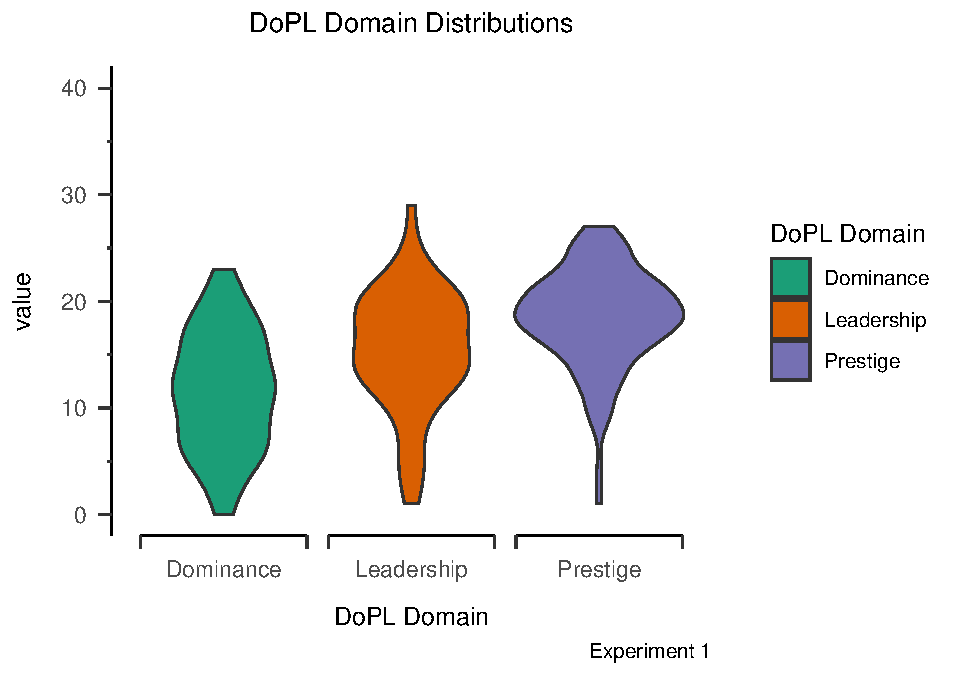
\includegraphics{Output_Files/Dissertation_files/figure-latex/DoPL-Experiment-1-1.pdf}
\caption{\label{fig:DoPL-Experiment-1}Violin plot visually showing the distribution of dominance, prestige, and leadership of participants in experiment 1. As seen in the figure, of participants within each power orientation dominance oriented people are more evenly distributed while those that were more prestige and leadership oriented were tended to be more prestigous oriented than others.}
\end{figure}

\begin{figure}

{\centering 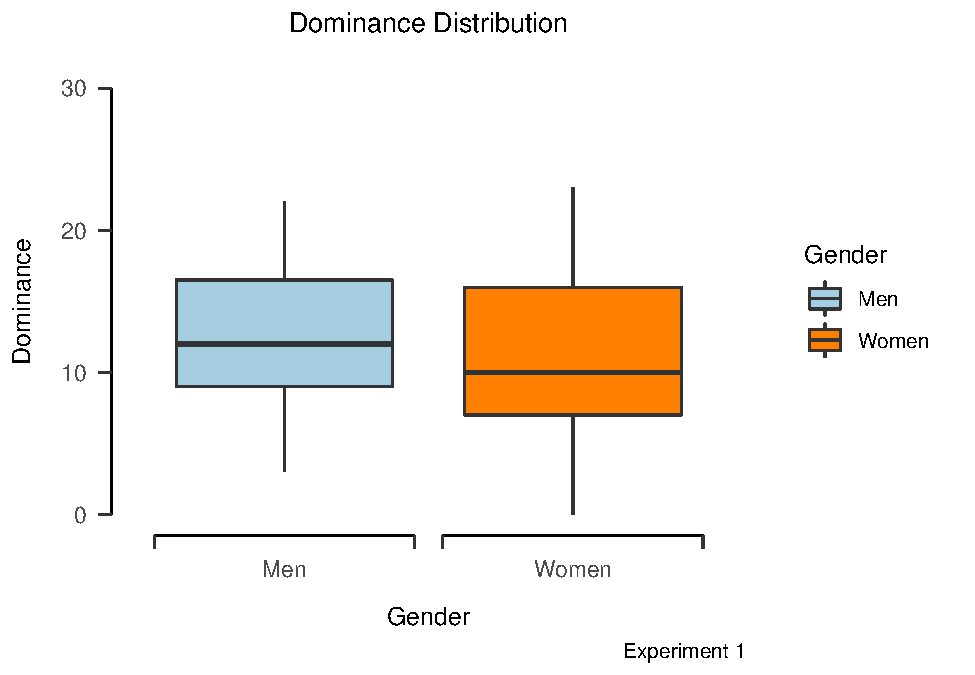
\includegraphics{Output_Files/Dissertation_files/figure-latex/DominanceExperiment1-1} 

}

\caption{Depicted is the gender distribution of Men and Women with regard to level of dominance. As can be seen, men are slightly higher in dominance then women.}\label{fig:DominanceExperiment1}
\end{figure}

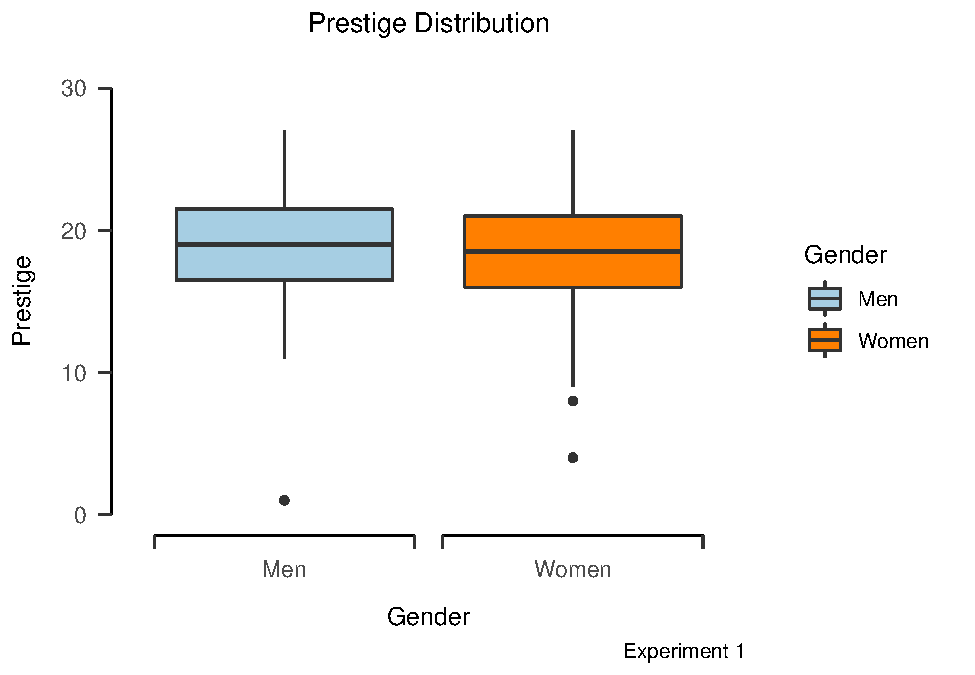
\includegraphics{Output_Files/Dissertation_files/figure-latex/PrestigeExperiment1-1.pdf}
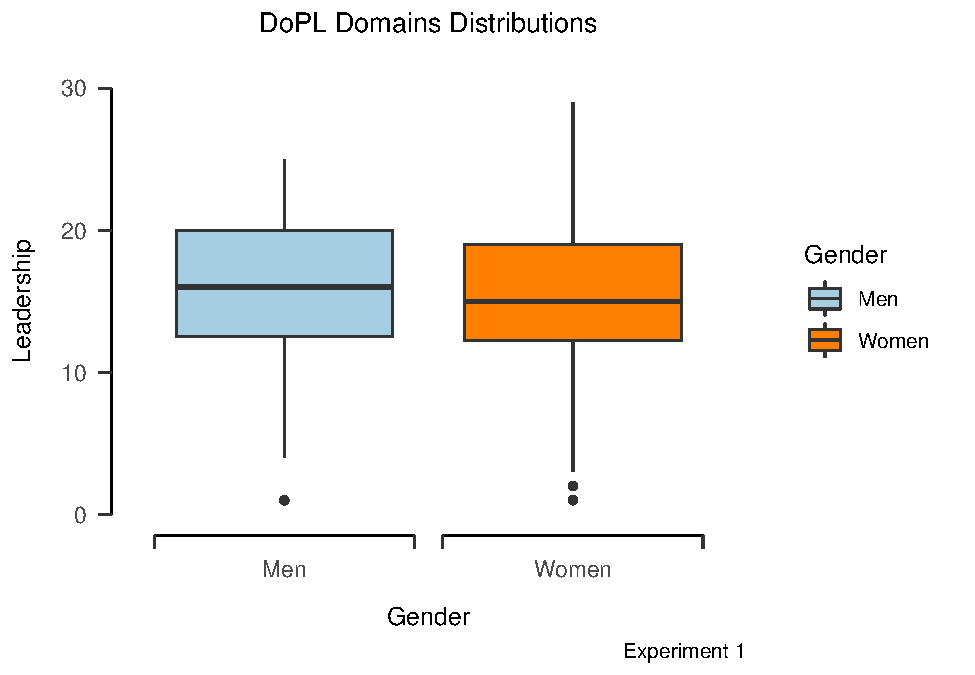
\includegraphics{Output_Files/Dissertation_files/figure-latex/LeadershipExperiment1-1.pdf}

\begin{verbatim}
## Warning: Removed 281 rows containing non-finite values (stat_ydensity).
\end{verbatim}

\begin{verbatim}
## Warning: Removed 281 rows containing missing values (geom_point).
\end{verbatim}

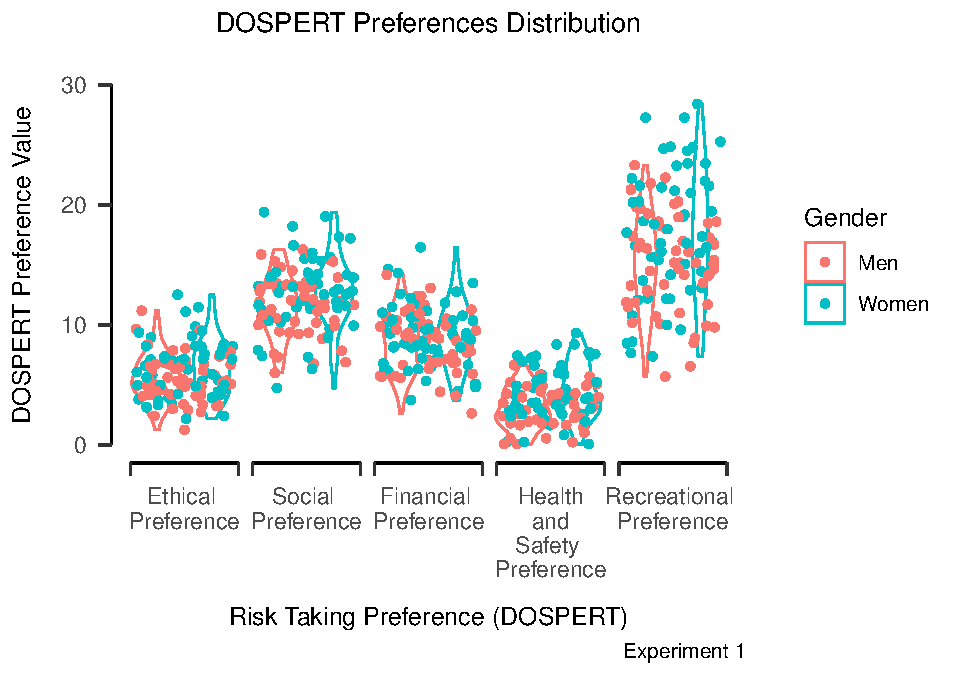
\includegraphics{Output_Files/Dissertation_files/figure-latex/DOSPERT-Preferences-GenderExperiment1-1.pdf}
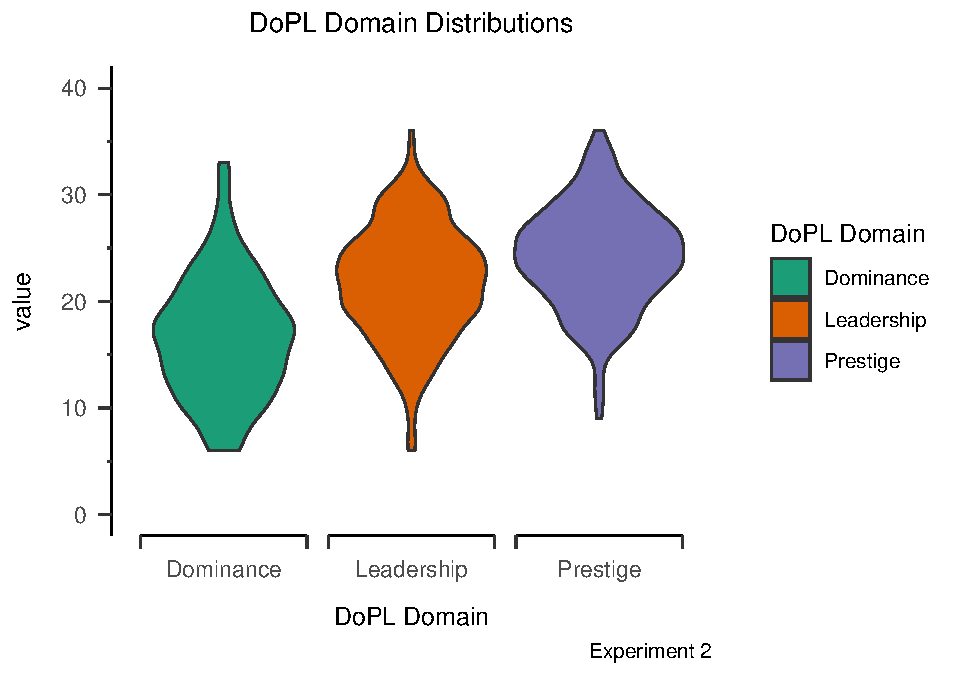
\includegraphics{Output_Files/Dissertation_files/figure-latex/DoPLDomainsExperiment2-1.pdf}

\begin{verbatim}
## Warning: Removed 752 rows containing non-finite values (stat_ydensity).
\end{verbatim}

\begin{verbatim}
## Warning: Removed 752 rows containing missing values (geom_point).
\end{verbatim}

\begin{figure}
\centering
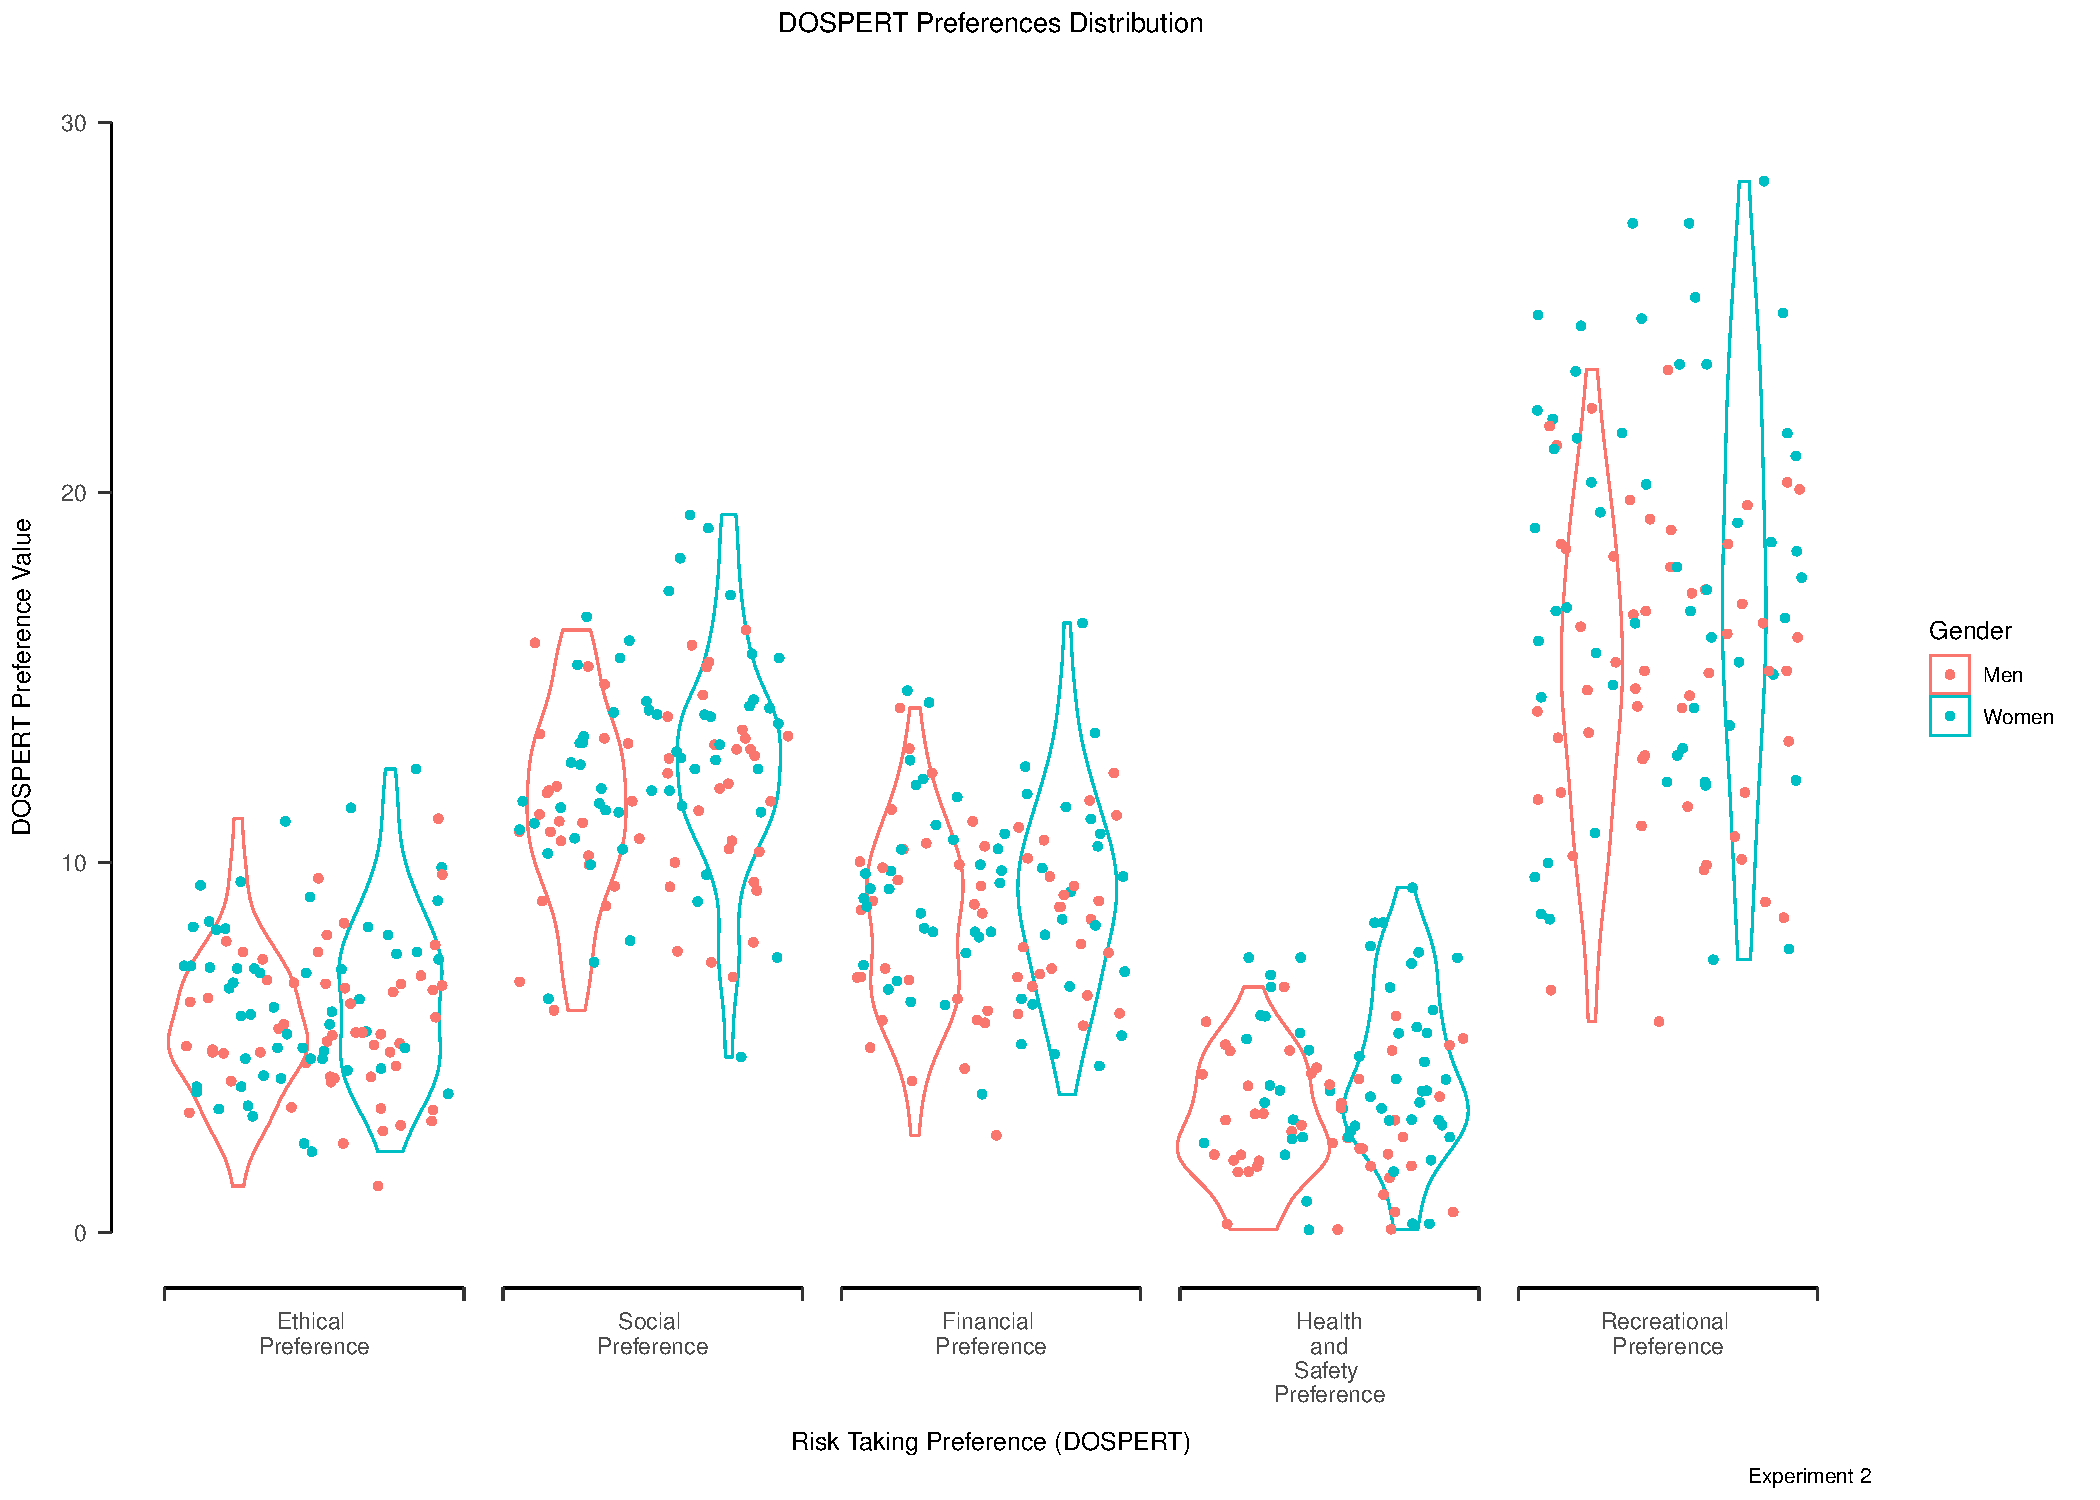
\includegraphics{Output_Files/Dissertation_files/figure-latex/DOSPERT-Preferences-GenderExperiment2-1.pdf}
\caption{\label{fig:DOSPERT-Preferences-GenderExperiment2}Depicted is the gender distribution of Men and Women with regard to each sub-domain of the domain specific risk-taking scale.}
\end{figure}

\begin{verbatim}
## Warning: Continuous limits supplied to discrete scale.
## Did you mean `limits = factor(...)` or `scale_*_continuous()`?
\end{verbatim}

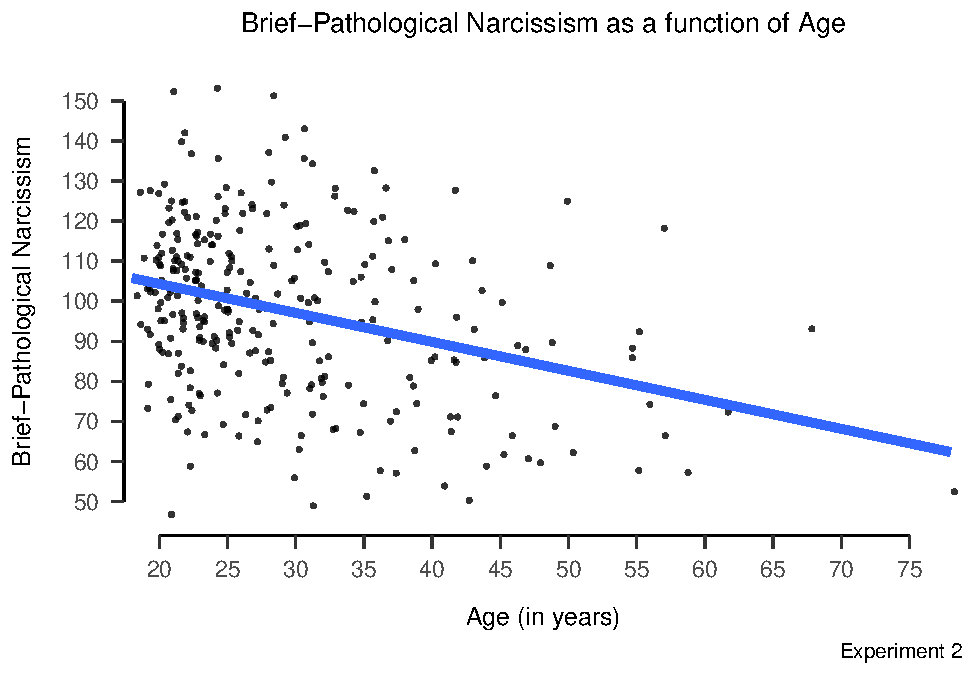
\includegraphics{Output_Files/Dissertation_files/figure-latex/Experiment-2-PNI-distribution-1.pdf}
\newpage

\begin{landscape}
\begin{figure}

{\centering 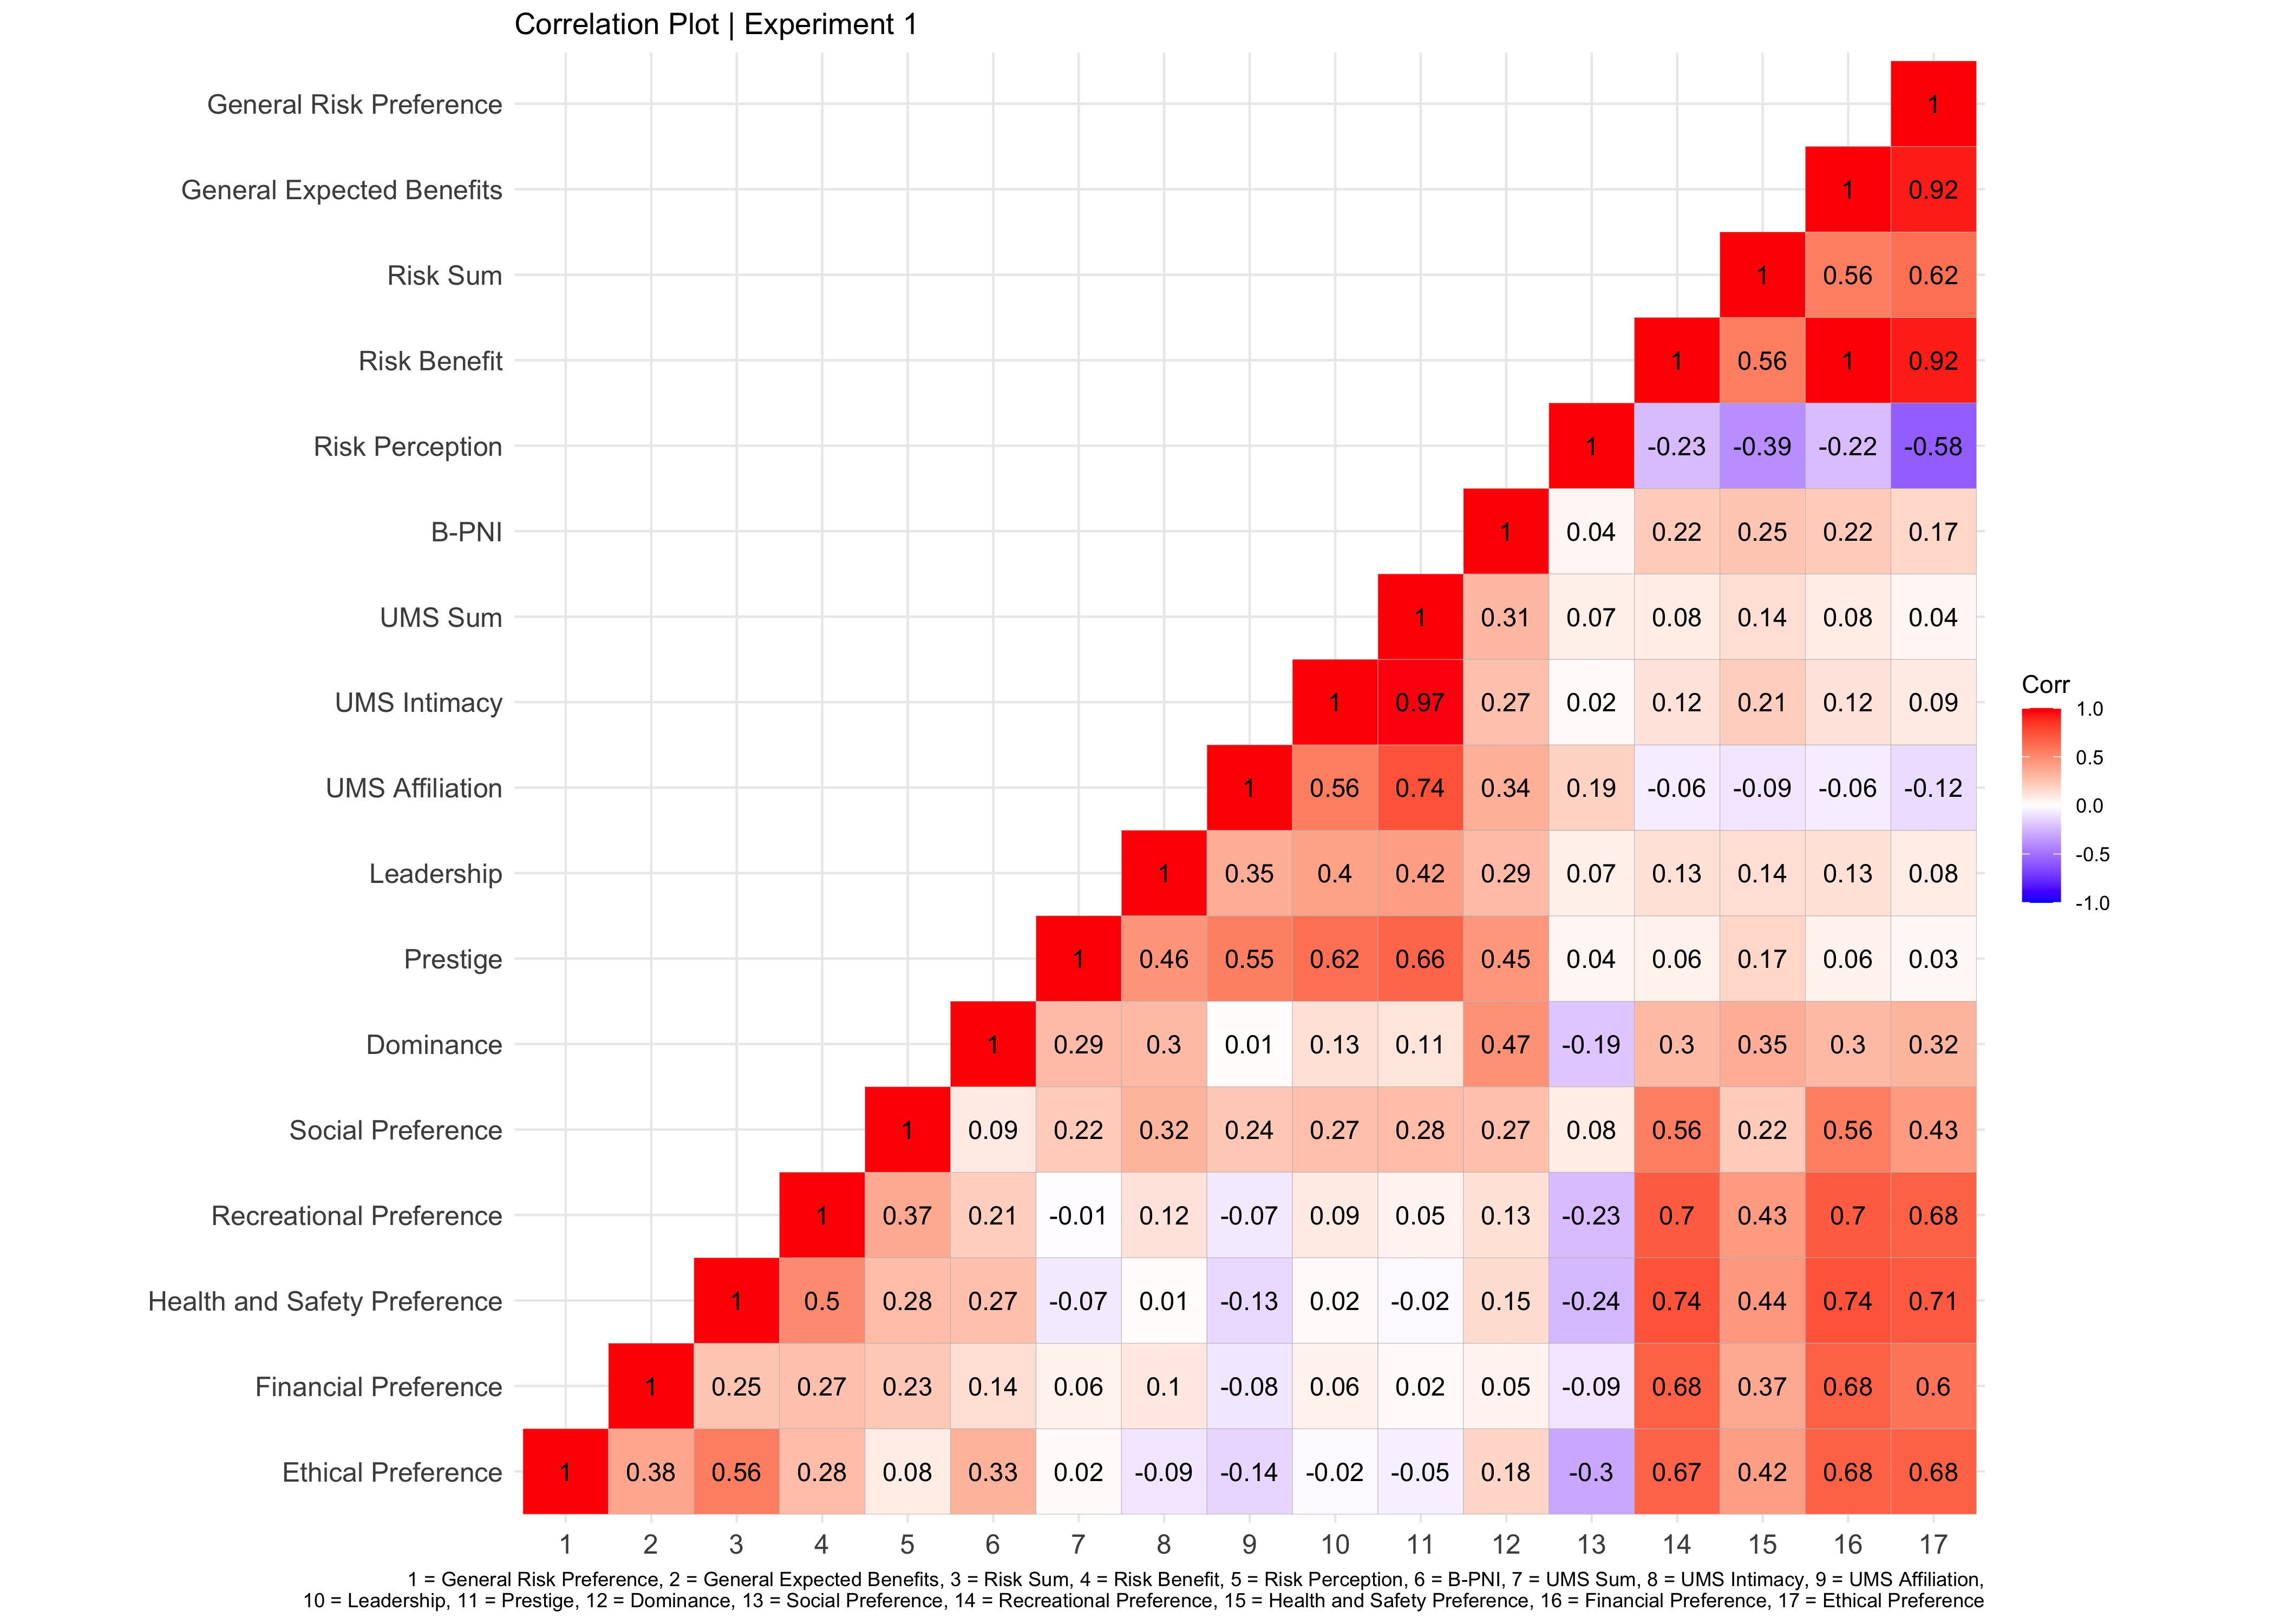
\includegraphics{Output_Files/Dissertation_files/figure-latex/correlationExperiment1-1} 

}

\caption{Depicted here is a correlation plot of the indices of experiment 1. The legend denotes stronger positive correlation (closer to 1 and darker red) or stronger negative correlation (closer to -1 and darker blue).}\label{fig:correlationExperiment1}
\end{figure}
\newpage
\begin{figure}

{\centering 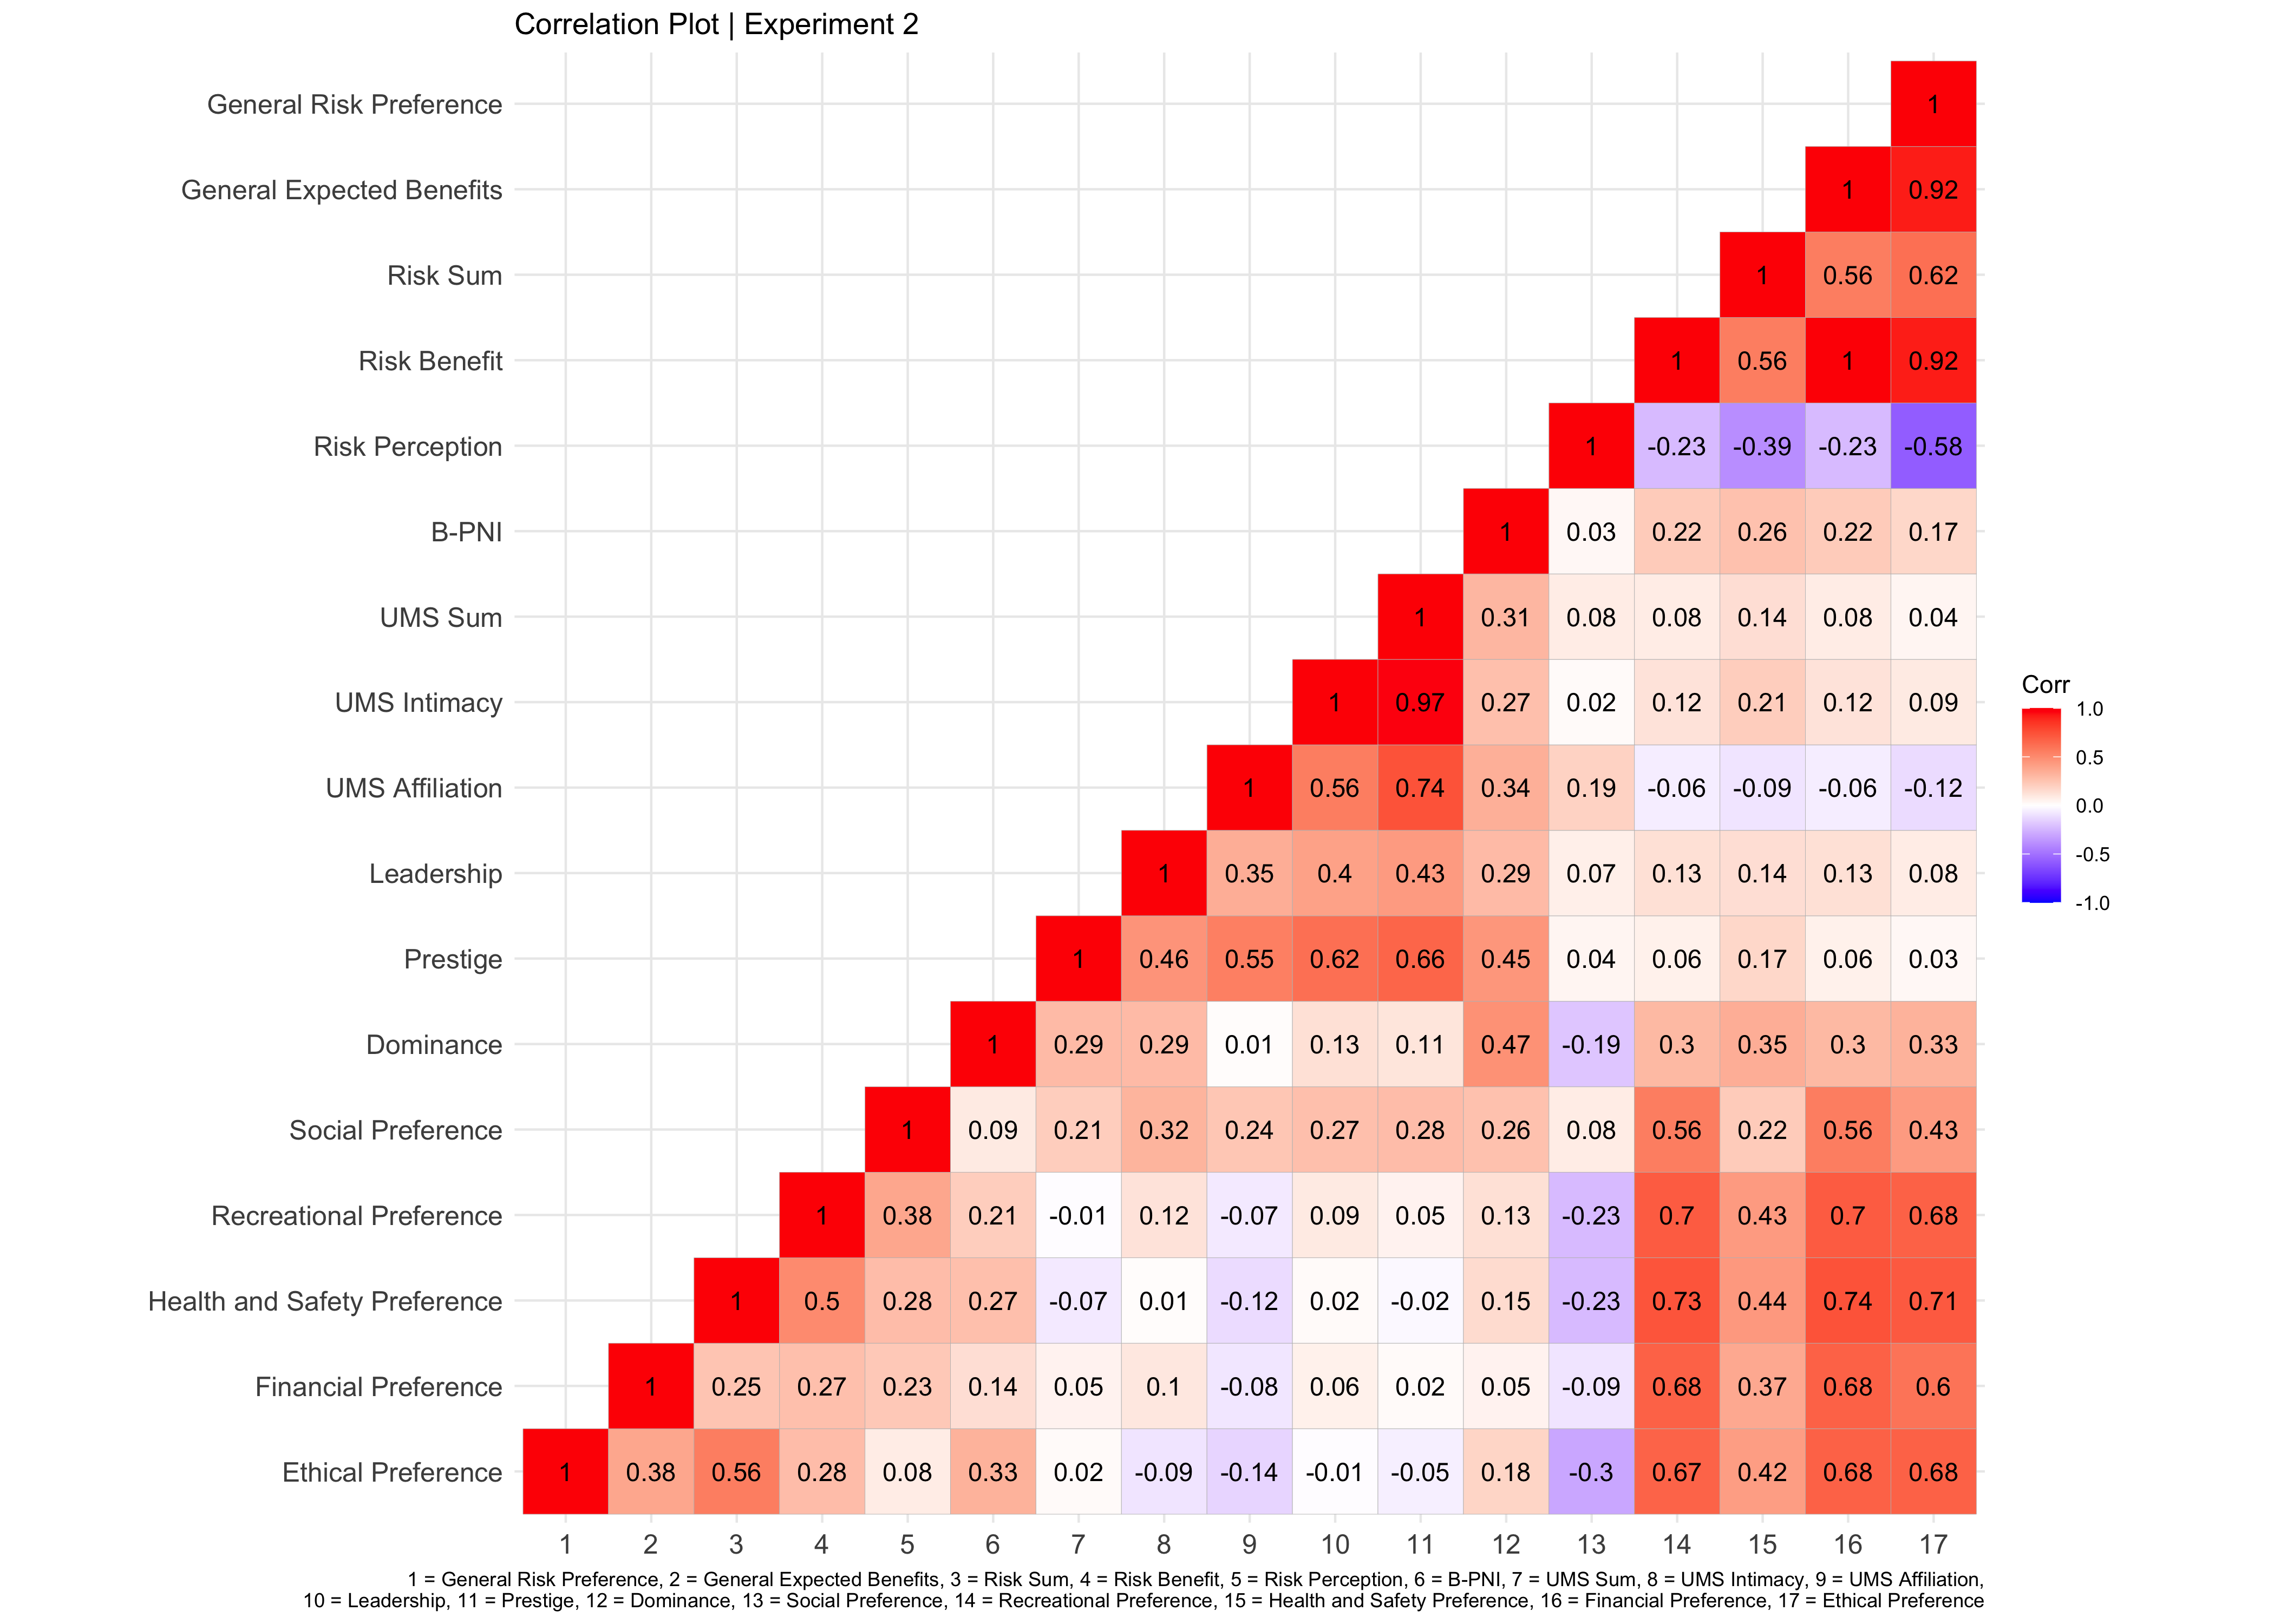
\includegraphics{Output_Files/Dissertation_files/figure-latex/correlationExperiment2-1} 

}

\caption{Depicted here is a correlation plot of the indices of experiment 2. The legend denotes stronger positive correlation (closer to 1 and darker red) or stronger negative correlation (closer to -1 and darker blue).}\label{fig:correlationExperiment2}
\end{figure}
\end{landscape}
\newpage
\begin{figure}

{\centering 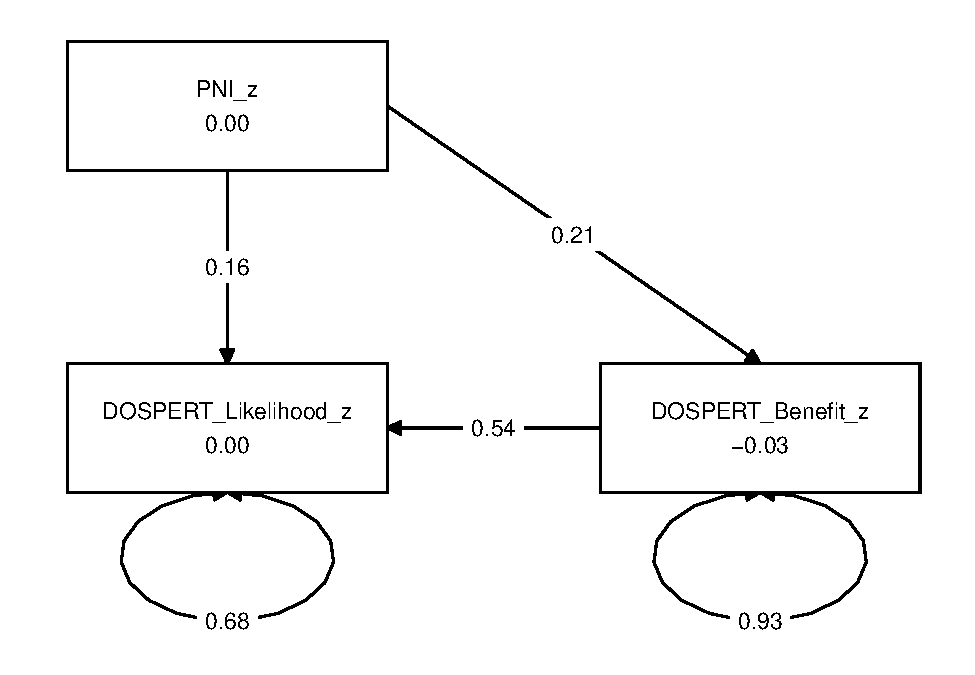
\includegraphics[width=1\linewidth]{Output_Files/Dissertation_files/figure-latex/MediationFit1-1} 

}

\caption{Figure represents a mediation model with Narcissism as the central mediator in the model.The outcome variables being risk likelihood.}\label{fig:MediationFit1}
\end{figure}
\begin{figure}

{\centering 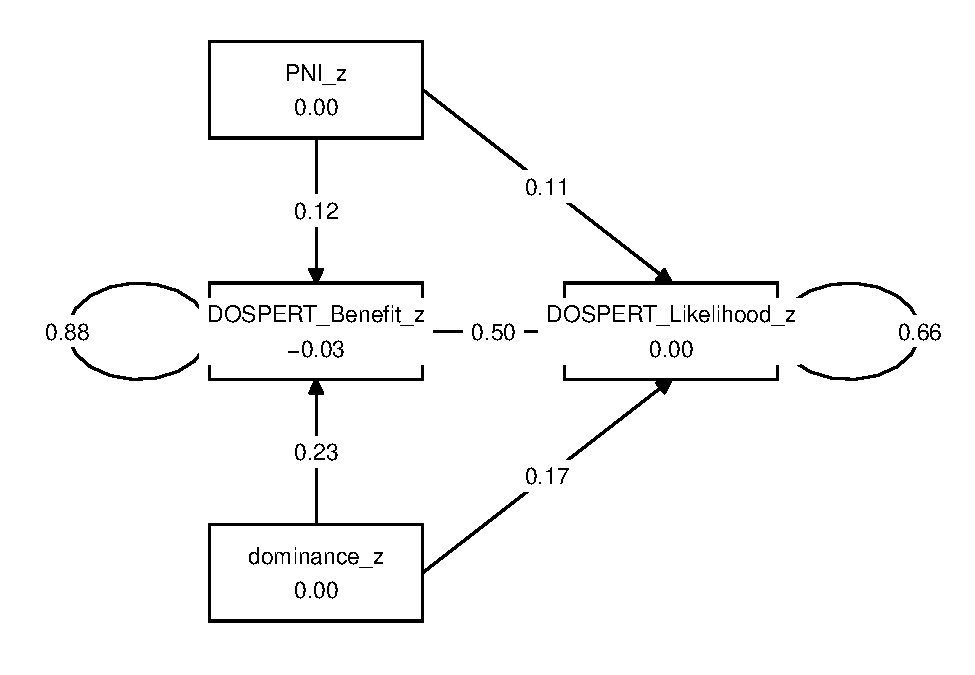
\includegraphics[width=1\linewidth]{Output_Files/Dissertation_files/figure-latex/MediationFit2-1} 

}

\caption{Figure represents a mediation model with Narcissism and Dominance as the central mediators in a parallel model.The outcome variables being risk likelihood.}\label{fig:MediationFit2}
\end{figure}
\begin{figure}

{\centering 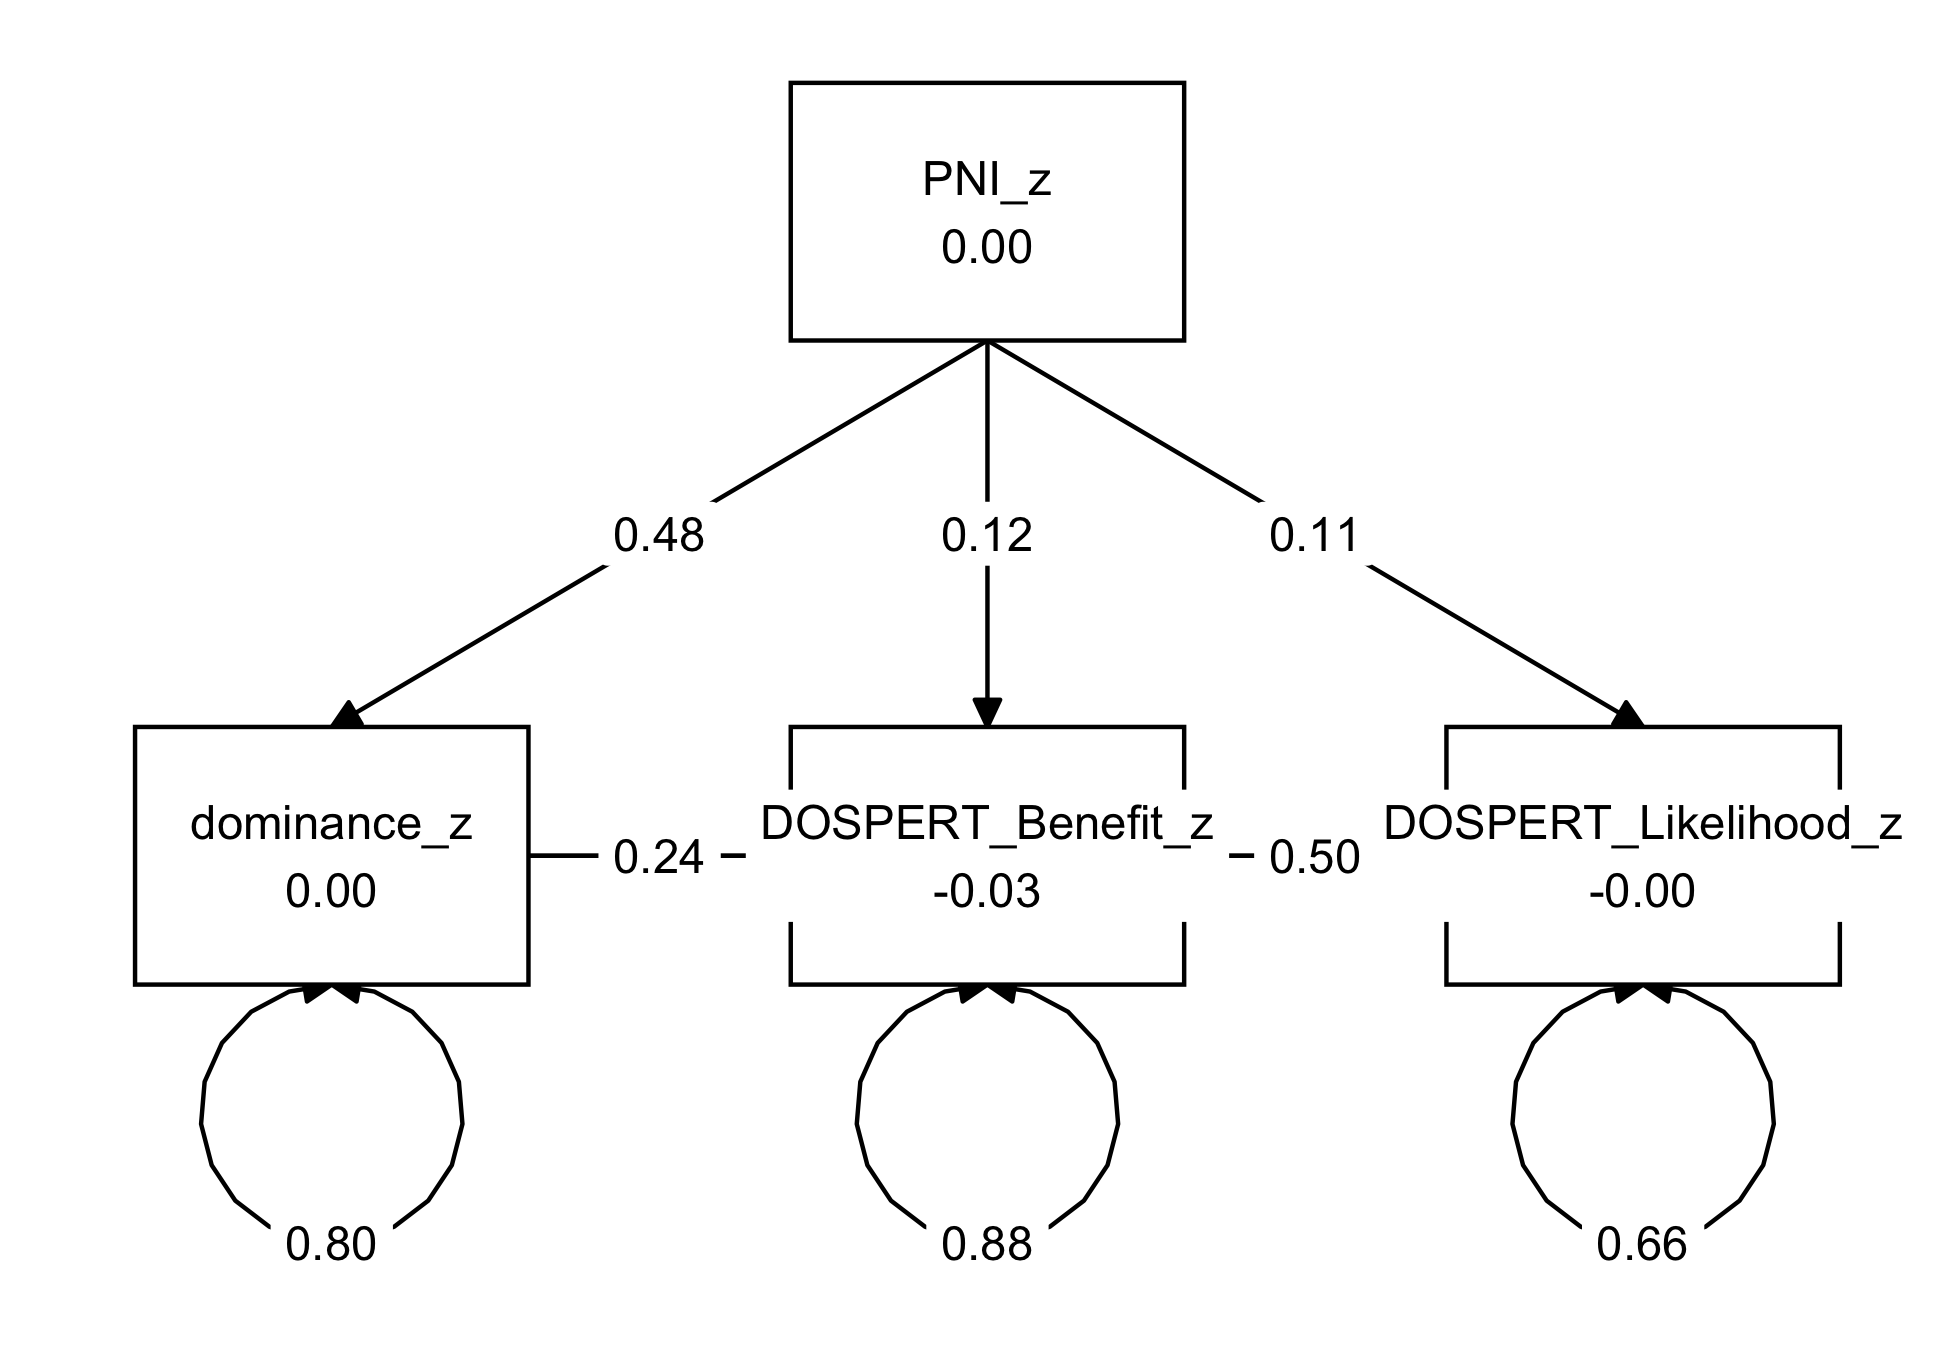
\includegraphics[width=1\linewidth]{Output_Files/Dissertation_files/figure-latex/MediationFit3-1} 

}

\caption{Figure represents a mediation model with Narcissism and Dominance as the moderator in a serial model.The outcome variables being risk likelihood.}\label{fig:MediationFit3}
\end{figure}

\newpage

\begin{table}[ht]

\begin{center}
\begin{threeparttable}

\caption{\label{tab:m1-fixef-Experiment-1}Fixed Effects: DoPL * General Risk}

\begin{tabular}{llll}
\toprule
Parameter & \multicolumn{1}{c}{Estimate} & \multicolumn{1}{c}{Est.Error} & \multicolumn{1}{c}{CI (95\%)}\\
\midrule
Intercept & 0.26 & 0.12 & 0.02 - 0.5\\
Dominance & 0.26 & 0.10 & 0.07 - 0.46\\
Gender & -0.55 & 0.16 & -0.87 - -0.23\\
\bottomrule
\addlinespace
\end{tabular}

\begin{tablenotes}[para]
\normalsize{\textit{Note.} The above represents fixed effects, confidence interevals low and high for a basic bayesian model of Dominance, Prestige, and Leadership predicting general risk preference. Matching signs for confidence intervals is displayed in the table.}
\end{tablenotes}

\end{threeparttable}
\end{center}

\end{table}

\begin{center}
\begin{ThreePartTable}

\begin{TableNotes}[para]
\normalsize{\textit{Note.} Fixed effect results of Dominance, Prestige, and Leadership with gender interactions predicting each of the individual Domain Specific Risk Taking (DOSPERT) domains.}
\end{TableNotes}

\begin{longtable}{llll}\noalign{\getlongtablewidth\global\LTcapwidth=\longtablewidth}
\caption{\label{tab:m3_exp_1}DOSPERT and DoPL Interaction: Experiment 1}\\
\toprule
Parameter & \multicolumn{1}{c}{Estimate} & \multicolumn{1}{c}{Est.Error} & \multicolumn{1}{c}{CI (95\%)}\\
\midrule
\endfirsthead
\caption*{\normalfont{Table \ref{tab:m3_exp_1} continued}}\\
\toprule
Parameter & \multicolumn{1}{c}{Estimate} & \multicolumn{1}{c}{Est.Error} & \multicolumn{1}{c}{CI (95\%)}\\
\midrule
\endhead
DOSPERT Recreation Preference * Intercept & 0.33 & 0.12 & 0.11 - 0.56\\
DOSPERT Ethical Preference * Dominance & 0.42 & 0.08 & 0.26 - 0.58\\
DOSPERT Financial Preference * Dominance & 0.22 & 0.08 & 0.06 - 0.38\\
DOSPERT Social Preference * Dominance & 0.24 & 0.08 & 0.07 - 0.4\\
DOSPERT Social Preference * Gender & -0.39 & 0.18 & -0.75 - -0.03\\
DOSPERT Health And Safety Preference * Dominance & 0.37 & 0.08 & 0.21 - 0.53\\
DOSPERT Recreation Preference * Dominance & 0.47 & 0.08 & 0.32 - 0.62\\
DOSPERT Recreation Preference * Gender & -0.70 & 0.17 & -1.03 - -0.38\\
DOSPERT Recreation Preference * Age & 0.22 & 0.09 & 0.06 - 0.39\\
\bottomrule
\addlinespace
\insertTableNotes
\end{longtable}

\end{ThreePartTable}
\end{center}

\begin{center}
\begin{ThreePartTable}

\begin{TableNotes}[para]
\normalsize{\textit{Note.} Fixed effect results of Dominance, Prestige, and Leadership with gender interactions predicting the perceptions and benefits of risk.}
\end{TableNotes}

\begin{longtable}{llll}\noalign{\getlongtablewidth\global\LTcapwidth=\longtablewidth}
\caption{\label{tab:m5-int-fixef-exp-1}DOSPERT Benefit and Perception: Experiment 1}\\
\toprule
Parameter & \multicolumn{1}{c}{Estimate} & \multicolumn{1}{c}{Est.Error} & \multicolumn{1}{c}{CI (95\%)}\\
\midrule
\endfirsthead
\caption*{\normalfont{Table \ref{tab:m5-int-fixef-exp-1} continued}}\\
\toprule
Parameter & \multicolumn{1}{c}{Estimate} & \multicolumn{1}{c}{Est.Error} & \multicolumn{1}{c}{CI (95\%)}\\
\midrule
\endhead
DOSPERT Risk Likelihood * Intercept & 0.25 & 0.11 & 0.03 - 0.47\\
DOSPERT Risk Perception * Intercept & -0.25 & 0.13 & -0.5 - -0.01\\
DOSPERT Risk Benefit * Intercept & 0.26 & 0.12 & 0.01 - 0.5\\
DOSPERT Risk Likelihood * Dominance & 0.41 & 0.09 & 0.23 - 0.59\\
DOSPERT Risk Likelihood * Gender & -0.50 & 0.15 & -0.8 - -0.21\\
DOSPERT Risk Perception * Dominance & -0.28 & 0.10 & -0.49 - -0.08\\
DOSPERT Risk Perception * Gender & 0.45 & 0.17 & 0.12 - 0.77\\
DOSPERT Risk Benefit * Dominance & 0.26 & 0.10 & 0.08 - 0.46\\
DOSPERT Risk Benefit * Gender & -0.57 & 0.16 & -0.88 - -0.27\\
\bottomrule
\addlinespace
\insertTableNotes
\end{longtable}

\end{ThreePartTable}
\end{center}

\begin{center}
\begin{ThreePartTable}

\begin{TableNotes}[para]
\normalsize{\textit{Note.} Fixed effect results of Dominance, Prestige, and Leadership with gender interactions predicting the perceptions and benefits of risk.}
\end{TableNotes}

\begin{longtable}{llll}\noalign{\getlongtablewidth\global\LTcapwidth=\longtablewidth}
\caption{\label{tab:m4-perceivedRisk-Gender-exp-1}DOSPERT Benefit and Perception: Experiment 1}\\
\toprule
Parameter & \multicolumn{1}{c}{Estimate} & \multicolumn{1}{c}{Est.Error} & \multicolumn{1}{c}{CI (95\%)}\\
\midrule
\endfirsthead
\caption*{\normalfont{Table \ref{tab:m4-perceivedRisk-Gender-exp-1} continued}}\\
\toprule
Parameter & \multicolumn{1}{c}{Estimate} & \multicolumn{1}{c}{Est.Error} & \multicolumn{1}{c}{CI (95\%)}\\
\midrule
\endhead
DOSPERT Risk Likelihood * Dominance & 0.65 & 0.13 & 0.39 - 0.91\\
DOSPERT Risk Likelihood * Gender & -0.48 & 0.15 & -0.77 - -0.19\\
DOSPERT Risk Likelihood * Dominance : Gender & -0.49 & 0.18 & -0.84 - -0.14\\
DOSPERT Risk Perception * Dominance & -0.30 & 0.15 & -0.6 - -0.02\\
DOSPERT Risk Perception * Gender & 0.44 & 0.16 & 0.12 - 0.77\\
DOSPERT Risk Benefit * Dominance & 0.40 & 0.14 & 0.13 - 0.68\\
DOSPERT Risk Benefit * Gender & -0.56 & 0.16 & -0.88 - -0.25\\
\bottomrule
\addlinespace
\insertTableNotes
\end{longtable}

\end{ThreePartTable}
\end{center}

\begin{table}[ht]

\begin{center}
\begin{threeparttable}

\caption{\label{tab:PNI-Model-DoPL-Exp-2}General Risk * DoPL: Experiment 2}

\begin{tabular}{llll}
\toprule
Parameter & \multicolumn{1}{c}{Estimate} & \multicolumn{1}{c}{Est.Error} & \multicolumn{1}{c}{CI (95\%)}\\
\midrule
Intercept & 0.75 & 0.19 & 0.38 - 1.11\\
Dominance & 0.33 & 0.08 & 0.17 - 0.49\\
Age & -0.02 & 0.01 & -0.04 - -0.01\\
\bottomrule
\addlinespace
\end{tabular}

\begin{tablenotes}[para]
\normalsize{\textit{Note.} Fixed effect results of Dominance, Prestige, and Leadership with gender interactions predicting general risk preference.}
\end{tablenotes}

\end{threeparttable}
\end{center}

\end{table}

\begin{center}
\begin{ThreePartTable}

\begin{TableNotes}[para]
\normalsize{\textit{Note.} Fixed effect results of Narcisism as a mediation in a model predicting risk likelihood through risk benefit.}
\end{TableNotes}

\begin{longtable}{llll}\noalign{\getlongtablewidth\global\LTcapwidth=\longtablewidth}
\caption{\label{tab:MediationBRMS1Exp2}DOSPERT Risk Likelihood and Benefit Mediation: Experiment 2}\\
\toprule
Parameter & \multicolumn{1}{c}{Estimate} & \multicolumn{1}{c}{Est.Error} & \multicolumn{1}{c}{CI (95\%)}\\
\midrule
\endfirsthead
\caption*{\normalfont{Table \ref{tab:MediationBRMS1Exp2} continued}}\\
\toprule
Parameter & \multicolumn{1}{c}{Estimate} & \multicolumn{1}{c}{Est.Error} & \multicolumn{1}{c}{CI (95\%)}\\
\midrule
\endhead
DOSPERT Risk Likelihood * DOSPERT Risk Benefit & 0.54 & 0.05 & 0.44 - 0.63\\
DOSPERT Risk Likelihood * PNI & 0.16 & 0.04 & 0.07 - 0.24\\
DOSPERT Risk Benefit * PNI & 0.21 & 0.05 & 0.11 - 0.31\\
\bottomrule
\addlinespace
\insertTableNotes
\end{longtable}

\end{ThreePartTable}
\end{center}

\begin{center}
\begin{ThreePartTable}

\begin{TableNotes}[para]
\normalsize{\textit{Note.} Fixed effect results of Narcisism and Dominance as a mediation in a model predicting risk likelihood through risk benefit.}
\end{TableNotes}

\begin{longtable}{llll}\noalign{\getlongtablewidth\global\LTcapwidth=\longtablewidth}
\caption{\label{tab:MediationBRMS2Exp2}DOSPERT Risk Likelihood and Benefit Mediation: Experiment 2}\\
\toprule
Parameter & \multicolumn{1}{c}{Estimate} & \multicolumn{1}{c}{Est.Error} & \multicolumn{1}{c}{CI (95\%)}\\
\midrule
\endfirsthead
\caption*{\normalfont{Table \ref{tab:MediationBRMS2Exp2} continued}}\\
\toprule
Parameter & \multicolumn{1}{c}{Estimate} & \multicolumn{1}{c}{Est.Error} & \multicolumn{1}{c}{CI (95\%)}\\
\midrule
\endhead
DOSPERT Risk Likelihood * DOSPERT Risk Benefit & 0.50 & 0.05 & 0.4 - 0.6\\
DOSPERT Risk Likelihood * PNI & 0.11 & 0.05 & 0.02 - 0.2\\
DOSPERT Risk Likelihood * Dominance & 0.16 & 0.05 & 0.05 - 0.26\\
DOSPERT Risk Benefit * PNI & 0.12 & 0.05 & 0.02 - 0.23\\
DOSPERT Risk Benefit * Dominance & 0.24 & 0.06 & 0.12 - 0.36\\
\bottomrule
\addlinespace
\insertTableNotes
\end{longtable}

\end{ThreePartTable}
\end{center}

\begin{center}
\begin{ThreePartTable}

\begin{TableNotes}[para]
\normalsize{\textit{Note.} Fixed effect results of Narcisism and Dominance as a mediation in a model predicting risk likelihood through risk benefit.}
\end{TableNotes}

\begin{longtable}{llll}\noalign{\getlongtablewidth\global\LTcapwidth=\longtablewidth}
\caption{\label{tab:MediationBRMS3Exp2}DOSPERT Risk Likelihood and Benefit Mediation: Experiment 2}\\
\toprule
Parameter & \multicolumn{1}{c}{Estimate} & \multicolumn{1}{c}{Est.Error} & \multicolumn{1}{c}{CI (95\%)}\\
\midrule
\endfirsthead
\caption*{\normalfont{Table \ref{tab:MediationBRMS3Exp2} continued}}\\
\toprule
Parameter & \multicolumn{1}{c}{Estimate} & \multicolumn{1}{c}{Est.Error} & \multicolumn{1}{c}{CI (95\%)}\\
\midrule
\endhead
DOSPERT Risk Likelihood * DOSPERT Risk Benefit & 0.50 & 0.05 & 0.41 - 0.6\\
DOSPERT Risk Likelihood * Dominance & 0.16 & 0.05 & 0.06 - 0.27\\
DOSPERT Risk Likelihood * PNI & 0.10 & 0.05 & 0.02 - 0.19\\
DOSPERT Risk Benefit * PNI & 0.12 & 0.05 & 0.02 - 0.23\\
DOSPERT Risk Benefit * Dominance & 0.24 & 0.05 & 0.13 - 0.35\\
Dominance * PNI & 0.48 & 0.05 & 0.37 - 0.58\\
\bottomrule
\addlinespace
\insertTableNotes
\end{longtable}

\end{ThreePartTable}
\end{center}

\begin{lltable}

\begin{TableNotes}[para]
\normalsize{\textit{Note.}  * denotes significance level. 1 = DOSPERT General Preference, 2 = DOSPERT Recreation Preference, 3 = DOSPERT Health/Safety Preference, 4 = DOSPERT Social Preference, 5 = DOSPERT Financial Preference, 6 = DOSPERT Ethical Preference, 7 = DOSPERT Risk Benefit, 8 = DOSPERT Risk Perception, 9 = DOSPERT Risk Likelihood, 10 = UMS Affiliation, 11 = UMS Intimacy, 12 = UMS, 13 = Leadership, 14 = Prestige, 15 = Dominance, 16 = DoPL}
\end{TableNotes}

\tiny{

\begin{longtable}{lllllllllllllllll}\noalign{\getlongtablewidth\global\LTcapwidth=\longtablewidth}
\caption{\label{tab:unnamed-chunk-11}General Correlation Matrix | Experiment 2}\\
\toprule
Parameter & 1 & 2 & 3 & 4 & 5 & 6 & 7 & 8 & 9 & 10 & 11 & 12 & 13 & 14 & 15 & 16\\
\midrule
\endfirsthead
\caption*{\normalfont{Table \ref{tab:unnamed-chunk-11} continued}}\\
\toprule
Parameter & 1 & 2 & 3 & 4 & 5 & 6 & 7 & 8 & 9 & 10 & 11 & 12 & 13 & 14 & 15 & 16\\
\midrule
\endhead
DoPL & 0.26** & 0.20* & 0.21* & 0.27** & 0.19* & 0.27** & 0.27** & 2.51E-03 & 0.41*** & 0.38*** & 0.24** & 0.38*** & 0.73*** & 0.73*** & 0.73*** & 1\\
Dominance & 0.26** & 0.31*** & 0.23** & 0.20* & 0.14 & 0.29*** & 0.25** & -0.12 & 0.42*** & 0.18 & 5.10E-03 & 0.13 & 0.27** & 0.37*** & 1 & \\
Prestige & 0.22** & 0.07 & 0.16 & 0.26** & 0.20* & 0.18* & 0.22** & 0.13 & 0.31*** & 0.38*** & 0.43*** & 0.45*** & 0.36*** & 1 &  & \\
Leadership & 0.13 & 0.05 & 0.08 & 0.17 & 0.09 & 0.14 & 0.12 & 0.02 & 0.19* & 0.31** & 0.16 & 0.29** & 1 &  &  & \\
UMS & 0.15 & -3.31E-03 & 0.14 & 0.17 & 0.22** & 0.05 & 0.16 & 0.23** & 0.23** & 0.95*** & 0.76*** & 1 &  &  &  & \\
UMS Intimacy & 0.06 & -0.07 & 0.06 & 0.1 & 0.11 & -0.04 & 0.07 & 0.26** & 0.06 & 0.53*** & 1 &  &  &  &  & \\
UMS Affiliation & 0.17 & 0.03 & 0.15 & 0.18* & 0.24** & 0.09 & 0.18* & 0.19* & 0.28** & 1 &  &  &  &  &  & \\
DOSPERT Risk Likelihood & 0.59*** & 0.49*** & 0.55*** & 0.55*** & 0.46*** & 0.55*** & 0.58*** & -0.17 & 1 &  &  &  &  &  &  & \\
DOSPERT Risk Perception & -0.09 & -0.34*** & -0.19* & -0.01 & 8.61E-04 & -0.16 & -0.05 & 1 &  &  &  &  &  &  &  & \\
DOSPERT Risk Benefit & 1.00*** & 0.82*** & 0.86*** & 0.84*** & 0.88*** & 0.87*** & 1 &  &  &  &  &  &  &  &  & \\
DOSPERT Ethical Preference & 0.88*** & 0.75*** & 0.77*** & 0.65*** & 0.69*** & 1 &  &  &  &  &  &  &  &  &  & \\
DOSPERT Financial Preference & 0.87*** & 0.67*** & 0.68*** & 0.67*** & 1 &  &  &  &  &  &  &  &  &  &  & \\
DOSPERT Social Preference & 0.84*** & 0.59*** & 0.69*** & 1 &  &  &  &  &  &  &  &  &  &  &  & \\
DOSPERT Health/Safety Preference & 0.87*** & 0.69*** & 1 &  &  &  &  &  &  &  &  &  &  &  &  & \\
DOSPERT Recreation Preference & 0.83*** & 1 &  &  &  &  &  &  &  &  &  &  &  &  &  & \\
DOSPERT General Preference & 1 &  &  &  &  &  &  &  &  &  &  &  &  &  &  & \\
\bottomrule
\addlinespace
\insertTableNotes
\end{longtable}

}

\end{lltable}

\begin{lltable}

\begin{TableNotes}[para]
\normalsize{\textit{Note.}  * denotes significance level. 1 = DOSPERT General Risk Preference, 2 = DOSPERT Recreation Preference, 3 = DOSPERT HS Preference, 4 = DOSPERT Social Preference, 5 = DOSPERT Financial Preference, 6 = DOSPERT Ethical Preference, 7 = DOSPERT Social Perception, 8 = DOSPERT Recreation Perception, 9 = DOSPERT HS Perception, 10 = DOSPERT Financial Perception, 11 = DOSPERT Ethical Perception, 12 = DOSPERT Social Benefit, 13 = DOSPERT Recreation Benefit, 14 = DOSPERT HS Benefit, 15 = DOSPERT Financial Benefit, 16 = DOSPERT Ethical Benefit, 17 = DOSPERT Social Likelihood, 18 = DOSPERT Recreation Likelihood, 19 = DOSPERT HS Likelihood, 20 = DOSPERT Financial Likelihood, 21 = DOSPERT Ethical Likelihood, 22 = DOSPERT Risk Benefit, 23 = DOSPERT Risk Perception, 24 = DOSPERT Risk Likelihood, 25 = UMS Affiliation, 26 = UMS Intimacy, 27 = UMS, 28 = Leadership, 29 = Prestige, 30 = Dominance, 31 = DoPL}
\end{TableNotes}

\tiny{

\begin{longtable}{llllllllllllllllllllllllllllllll}\noalign{\getlongtablewidth\global\LTcapwidth=\longtablewidth}
\caption{\label{tab:unnamed-chunk-12}General Correlation Matrix | Experiment 2}\\
\toprule
Parameter & 1 & 2 & 3 & 4 & 5 & 6 & 7 & 8 & 9 & 10 & 11 & 12 & 13 & 14 & 15 & 16 & 17 & 18 & 19 & 20 & 21 & 22 & 23 & 24 & 25 & 26 & 27 & 28 & 29 & 30 & 31\\
\midrule
\endfirsthead
\caption*{\normalfont{Table \ref{tab:unnamed-chunk-12} continued}}\\
\toprule
Parameter & 1 & 2 & 3 & 4 & 5 & 6 & 7 & 8 & 9 & 10 & 11 & 12 & 13 & 14 & 15 & 16 & 17 & 18 & 19 & 20 & 21 & 22 & 23 & 24 & 25 & 26 & 27 & 28 & 29 & 30 & 31\\
\midrule
\endhead
DoPL & 0.27** & 0.20* & 0.21* & 0.27*** & 0.19* & 0.27** & -2.47E-03 & -9.78E-03 & 0.03 & 0.03 & -0.04 & 0.27** & 0.22* & 0.22** & 0.19* & 0.28** & 0.28** & 0.30*** & 0.30*** & 0.34*** & 0.34*** & 0.26** & 3.53E-03 & 0.40*** & 0.38*** & 0.24** & 0.37*** & 0.74*** & 0.73*** & 0.73*** & 1\\
Dominance & 0.26** & 0.31*** & 0.23** & 0.20* & 0.14 & 0.29** & -0.02 & -0.13 & -0.08 & -0.1 & -0.20* & 0.20* & 0.30*** & 0.22** & 0.15 & 0.27** & 0.20* & 0.38*** & 0.34*** & 0.33*** & 0.38*** & 0.25** & -0.12 & 0.42*** & 0.18* & 8.23E-03 & 0.14 & 0.28** & 0.37*** & 1 & \\
Prestige & 0.21* & 0.07 & 0.16 & 0.26** & 0.21* & 0.17* & 0.05 & 0.14 & 0.11 & 0.11 & 0.12 & 0.27** & 0.13 & 0.18* & 0.19* & 0.20* & 0.27** & 0.17 & 0.28** & 0.25** & 0.28** & 0.22* & 0.13 & 0.31*** & 0.38*** & 0.43*** & 0.44*** & 0.36*** & 1 &  & \\
Leadership & 0.12 & 0.05 & 0.08 & 0.17 & 0.1 & 0.14 & -0.03 & -6.41E-03 & 0.06 & 0.08 & 8.96E-03 & 0.16 & 0.06 & 0.09 & 0.09 & 0.15 & 0.17 & 0.13 & 0.07 & 0.18 & 0.1 & 0.12 & 0.02 & 0.20* & 0.30** & 0.16 & 0.29*** & 1 &  &  & \\
UMS & 0.16 & -2.16E-03 & 0.14 & 0.17 & 0.22* & 0.06 & 0.11 & 0.23* & 0.18* & 0.22** & 0.28** & 0.17* & 0.07 & 0.17 & 0.20* & 0.1 & 0.18* & 0.12 & 0.17 & 0.22* & 0.24** & 0.16 & 0.23** & 0.23** & 0.95*** & 0.76*** & 1 &  &  &  & \\
UMS Intimacy & 0.06 & -0.07 & 0.07 & 0.09 & 0.11 & -0.04 & 0.13 & 0.28** & 0.17 & 0.22* & 0.32*** & 0.11 & 0.02 & 0.09 & 0.09 & 8.10E-03 & 0.1 & -0.08 & 0.06 & 0.07 & 0.06 & 0.07 & 0.26** & 0.06 & 0.53*** & 1 &  &  &  &  & \\
UMS Affiliation & 0.17* & 0.03 & 0.15 & 0.17 & 0.24** & 0.09 & 0.08 & 0.16 & 0.16 & 0.19* & 0.21* & 0.18* & 0.08 & 0.18* & 0.22* & 0.13 & 0.19* & 0.19* & 0.19* & 0.26** & 0.29** & 0.18* & 0.18* & 0.28** & 1 &  &  &  &  &  & \\
DOSPERT Risk Likelihood & 0.59*** & 0.48*** & 0.55*** & 0.55*** & 0.46*** & 0.54*** & -0.22* & -0.17 & -0.13 & -0.06 & -0.14 & 0.54*** & 0.48*** & 0.55*** & 0.47*** & 0.54*** & 0.54*** & 0.80*** & 0.79*** & 0.80*** & 0.83*** & 0.58*** & -0.16 & 1 &  &  &  &  &  &  & \\
DOSPERT Risk Perception & -0.1 & -0.34*** & -0.19* & -8.90E-03 & -1.32E-03 & -0.16 & 0.81*** & 0.85*** & 0.88*** & 0.83*** & 0.88*** & 0.06 & -0.1 & -0.07 & -0.07 & -0.04 & 0.06 & -0.17 & -0.21* & -0.06 & -0.07 & -0.05 & 1 &  &  &  &  &  &  &  & \\
DOSPERT Risk Benefit & 1.00*** & 0.82*** & 0.86*** & 0.84*** & 0.88*** & 0.87*** & -0.12 & -0.09 & -0.07 & 0.09 & -0.02 & 0.84*** & 0.88*** & 0.87*** & 0.88*** & 0.89*** & 0.84*** & 0.45*** & 0.51*** & 0.59*** & 0.47*** & 1 &  &  &  &  &  &  &  &  & \\
DOSPERT Ethical Likelihood & 0.47*** & 0.40*** & 0.42*** & 0.39*** & 0.40*** & 0.47*** & -0.06 & -0.1 & -0.05 & 0.02 & -0.12 & 0.39*** & 0.40*** & 0.42*** & 0.40*** & 0.47*** & 0.39*** & 0.60*** & 0.64*** & 0.60*** & 1 &  &  &  &  &  &  &  &  &  & \\
DOSPERT Financial Likelihood & 0.59*** & 0.44*** & 0.48*** & 0.54*** & 0.49*** & 0.56*** & -0.09 & -0.06 & -3.35E-03 & -0.08 & -0.03 & 0.54*** & 0.47*** & 0.49*** & 0.50*** & 0.58*** & 0.54*** & 0.55*** & 0.54*** & 1 &  &  &  &  &  &  &  &  &  &  & \\
DOSPERT HS Likelihood & 0.51*** & 0.40*** & 0.59*** & 0.42*** & 0.43*** & 0.46*** & -0.26** & -0.15 & -0.24** & -0.08 & -0.20* & 0.40*** & 0.40*** & 0.56*** & 0.44*** & 0.44*** & 0.40*** & 0.57*** & 1 &  &  &  &  &  &  &  &  &  &  &  & \\
DOSPERT Recreation Likelihood & 0.45*** & 0.49*** & 0.43*** & 0.37*** & 0.30** & 0.43*** & -0.1 & -0.24** & -0.1 & -0.13 & -0.14 & 0.37*** & 0.46*** & 0.43*** & 0.31*** & 0.42*** & 0.37*** & 1 &  &  &  &  &  &  &  &  &  &  &  &  & \\
DOSPERT Social Likelihood & 0.84*** & 0.58*** & 0.68*** & 1.00*** & 0.67*** & 0.65*** & -0.11 & 0.05 & 0.04 & 0.18 & 0.1 & 1.00*** & 0.66*** & 0.70*** & 0.66*** & 0.68*** & 1 &  &  &  &  &  &  &  &  &  &  &  &  &  & \\
DOSPERT Ethical Benefit & 0.89*** & 0.72*** & 0.76*** & 0.67*** & 0.72*** & 0.99*** & -0.03 & -0.09 & -0.03 & 0.09 & -0.09 & 0.68*** & 0.77*** & 0.78*** & 0.71*** & 1 &  &  &  &  &  &  &  &  &  &  &  &  &  &  & \\
DOSPERT Financial Benefit & 0.88*** & 0.70*** & 0.69*** & 0.66*** & 1.00*** & 0.69*** & -0.15 & -0.08 & -0.11 & 0.04 & 0.01 & 0.66*** & 0.75*** & 0.69*** & 1 &  &  &  &  &  &  &  &  &  &  &  &  &  &  &  & \\
DOSPERT HS Benefit & 0.88*** & 0.66*** & 0.99*** & 0.70*** & 0.70*** & 0.76*** & -0.13 & -0.11 & -0.09 & 0.06 & -0.04 & 0.70*** & 0.70*** & 1 &  &  &  &  &  &  &  &  &  &  &  &  &  &  &  &  & \\
DOSPERT Recreation Benefit & 0.88*** & 0.95*** & 0.69*** & 0.66*** & 0.75*** & 0.76*** & -0.1 & -0.16 & -0.09 & 1.22E-04 & -0.08 & 0.66*** & 1 &  &  &  &  &  &  &  &  &  &  &  &  &  &  &  &  &  & \\
DOSPERT Social Benefit & 0.84*** & 0.58*** & 0.68*** & 1.00*** & 0.67*** & 0.65*** & -0.11 & 0.05 & 0.04 & 0.18* & 0.1 & 1 &  &  &  &  &  &  &  &  &  &  &  &  &  &  &  &  &  &  & \\
DOSPERT Ethical Perception & -0.06 & -0.29** & -0.14 & 0.05 & 0.07 & -0.23** & 0.62*** & 0.73*** & 0.73*** & 0.67*** & 1 &  &  &  &  &  &  &  &  &  &  &  &  &  &  &  &  &  &  &  & \\
DOSPERT Financial Perception & 0.05 & -0.19* & -0.03 & 0.12 & 0.12 & -0.01 & 0.57*** & 0.66*** & 0.69*** & 1 &  &  &  &  &  &  &  &  &  &  &  &  &  &  &  &  &  &  &  &  & \\
DOSPERT HS Perception & -0.1 & -0.28*** & -0.23** & -0.02 & -0.05 & -0.14 & 0.70*** & 0.67*** & 1 &  &  &  &  &  &  &  &  &  &  &  &  &  &  &  &  &  &  &  &  &  & \\
DOSPERT Recreation Perception & -0.12 & -0.44*** & -0.20* & -7.75E-04 & -0.03 & -0.19* & 0.60*** & 1 &  &  &  &  &  &  &  &  &  &  &  &  &  &  &  &  &  &  &  &  &  &  & \\
DOSPERT Social Perception & -0.16 & -0.27** & -0.22** & -0.20* & -0.1 & -0.12 & 1 &  &  &  &  &  &  &  &  &  &  &  &  &  &  &  &  &  &  &  &  &  &  &  & \\
DOSPERT Ethical Preference & 0.88*** & 0.75*** & 0.77*** & 0.65*** & 0.69*** & 1 &  &  &  &  &  &  &  &  &  &  &  &  &  &  &  &  &  &  &  &  &  &  &  &  & \\
DOSPERT Financial Preference & 0.88*** & 0.68*** & 0.69*** & 0.67*** & 1 &  &  &  &  &  &  &  &  &  &  &  &  &  &  &  &  &  &  &  &  &  &  &  &  &  & \\
DOSPERT Social Preference & 0.84*** & 0.59*** & 0.69*** & 1 &  &  &  &  &  &  &  &  &  &  &  &  &  &  &  &  &  &  &  &  &  &  &  &  &  &  & \\
DOSPERT HS Preference & 0.87*** & 0.69*** & 1 &  &  &  &  &  &  &  &  &  &  &  &  &  &  &  &  &  &  &  &  &  &  &  &  &  &  &  & \\
DOSPERT Recreation Preference & 0.83*** & 1 &  &  &  &  &  &  &  &  &  &  &  &  &  &  &  &  &  &  &  &  &  &  &  &  &  &  &  &  & \\
DOSPERT General Risk Preference & 1 &  &  &  &  &  &  &  &  &  &  &  &  &  &  &  &  &  &  &  &  &  &  &  &  &  &  &  &  &  & \\
\bottomrule
\addlinespace
\insertTableNotes
\end{longtable}

}

\end{lltable}

\begin{lltable}

\begin{TableNotes}[para]
\normalsize{\textit{Note.}  * denotes significance level. 1 = General Risk Preference, 2 = General Expected Benefits, 3 = Risk Sum, 4 = Risk Benefit, 5 = Risk Perception, 6 = B-PNI, 7 = UMS Sum, 8 = UMS Intimacy, 9 = UMS Affiliation, 10 = Leadership, 11 = Prestige, 12 = Dominance, 13 = Social Preference, 14 = Recreational Preference, 15 = Health and Safety Preference, 16 = Financial Preference, 17 = Ethical Preference}
\end{TableNotes}

\tiny{

\begin{longtable}{p{3cm}rrrrrrrrrrrrrrrrr}\noalign{\getlongtablewidth\global\LTcapwidth=\longtablewidth}
\caption{\label{tab:experiment2Correlation_BPNI}General Correlation Matrix | Experiment 2}\\
\toprule
Parameter & 1 & 2 & 3 & 4 & 5 & 6 & 7 & 8 & 9 & 10 & 11 & 12 & 13 & 14 & 15 & 16 & 17\\
\midrule
\endfirsthead
\caption*{\normalfont{Table \ref{tab:experiment2Correlation_BPNI} continued}}\\
\toprule
Parameter & 1 & 2 & 3 & 4 & 5 & 6 & 7 & 8 & 9 & 10 & 11 & 12 & 13 & 14 & 15 & 16 & 17\\
\midrule
\endhead
Ethical Preference & 0.68*** & 0.67*** & 0.42*** & 0.68*** & -0.30*** & 0.18** & -0.05 & -0.02 & -0.14* & -0.1 & 0.02 & 0.33*** & 0.08 & 0.28*** & 0.56*** & 0.38*** & 1\\
Financial Preference & 0.60*** & 0.68*** & 0.37*** & 0.68*** & -0.09 & 0.05 & 0.02 & 0.06 & -0.08 & 0.1 & 0.06 & 0.14* & 0.23*** & 0.27*** & 0.25*** & 1 & \\
Health and Safety Preference & 0.71*** & 0.74*** & 0.44*** & 0.74*** & -0.24*** & 0.15** & -0.02 & 0.02 & -0.12* & 0.01 & -0.07 & 0.27*** & 0.28*** & 0.50*** & 1 &  & \\
Recreational Preference & 0.68*** & 0.70*** & 0.43*** & 0.70*** & -0.23*** & 0.13* & 0.05 & 0.09 & -0.07 & 0.12* & -0.01 & 0.21*** & 0.38*** & 1 &  &  & \\
Social Preference & 0.43*** & 0.56*** & 0.22*** & 0.56*** & 0.08 & 0.27*** & 0.28*** & 0.27*** & 0.24*** & 0.32*** & 0.22*** & 0.09 & 1 &  &  &  & \\
Dominance & 0.33*** & 0.30*** & 0.35*** & 0.30*** & -0.19*** & 0.47*** & 0.11* & 0.13* & 0.01 & 0.29*** & 0.30*** & 1 &  &  &  &  & \\
Prestige & 0.03 & 0.06 & 0.17** & 0.06 & 0.05 & 0.45*** & 0.66*** & 0.62*** & 0.55*** & 0.46*** & 1 &  &  &  &  &  & \\
Leadership & 0.08 & 0.13* & 0.14* & 0.13* & 0.07 & 0.29*** & 0.42*** & 0.40*** & 0.35*** & 1 &  &  &  &  &  &  & \\
UMS Affiliation & -0.12* & -0.06 & -0.09 & -0.06 & 0.19*** & 0.34*** & 0.74*** & 0.56*** & 1 &  &  &  &  &  &  &  & \\
UMS Intimacy & 0.09 & 0.12* & 0.21*** & 0.12* & 0.03 & 0.27*** & 0.97*** & 1 &  &  &  &  &  &  &  &  & \\
UMS Sum & 0.04 & 0.08 & 0.14** & 0.08 & 0.07 & 0.31*** & 1 &  &  &  &  &  &  &  &  &  & \\
B-PNI & 0.17** & 0.22*** & 0.26*** & 0.22*** & 0.04 & 1 &  &  &  &  &  &  &  &  &  &  & \\
Risk Perception & -0.58 & -0.23*** & -0.39*** & -0.23*** & 1 &  &  &  &  &  &  &  &  &  &  &  & \\
Risk Benefit & 0.92*** & 1.00*** & 0.56*** & 1 &  &  &  &  &  &  &  &  &  &  &  &  & \\
Risk Sum & 0.62*** & 0.56*** & 1 &  &  &  &  &  &  &  &  &  &  &  &  &  & \\
General Expected Benefits & 0.92*** & 1 &  &  &  &  &  &  &  &  &  &  &  &  &  &  & \\
General Risk Preference & 1 &  &  &  &  &  &  &  &  &  &  &  &  &  &  &  & \\
\bottomrule
\addlinespace
\insertTableNotes
\end{longtable}

}

\end{lltable}

\begin{lltable}

\begin{TableNotes}[para]
\normalsize{\textit{Note.} * denotes signficance level. 1 = Self-Sacrifing and Self-Enhancement, 2 = Grandiose Fantasy, 3 = Exploitativeness, 4 = Hiding the Self, 5 = Entitlement Rage, 6 = Devaluing, 7 = Contingent Self-Esteem, 8 = Vulnerability, 9 = Grandiosity , 10 = B-PNI , 11 = Prestige , 12 = Leadership, 13 = Dominance}
\end{TableNotes}

\scriptsize{

\begin{longtable}{llllllllllllll}\noalign{\getlongtablewidth\global\LTcapwidth=\longtablewidth}
\caption{\label{tab:experiment2Correlation_MPNI}General Correlation Matrix | Experiment 2}\\
\toprule
Parameter & 1 & 2 & 3 & 4 & 5 & 6 & 7 & 8 & 9 & 10 & 11 & 12 & 13\\
\midrule
\endfirsthead
\caption*{\normalfont{Table \ref{tab:experiment2Correlation_MPNI} continued}}\\
\toprule
Parameter & 1 & 2 & 3 & 4 & 5 & 6 & 7 & 8 & 9 & 10 & 11 & 12 & 13\\
\midrule
\endhead
Dominance\ \ \ \ \ \ \ \ \ \ \ \ \ \ & 0.18** & 0.15* & 0.49*** & 0.30*** & 0.52*** & 0.30*** & 0.34*** & 0.44*** & 0.36*** & 0.46*** & 0.29*** & 0.30*** & 1\\
Leadership\ \ \ \ \ \ \ \ \ \ \ \ & 0.30*** & 0.26*** & 0.51*** & 0.07 & 0.22*** & 0.04 & 0.05 & 0.12 & 0.48*** & 0.29*** & 0.46*** & 1 & \\
Prestige\ \ \ \ \ \ \ \ \ \ \ \ \ \ & 0.46*** & 0.38*** & 0.34*** & 0.16* & 0.40*** & 0.19** & 0.32*** & 0.32*** & 0.53*** & 0.45*** & 1 &  & \\
B-PNI\ \ \ \ \ \ \ \ \ \ \ \ \ \ \ \ \ \ & 0.65*** & 0.63*** & 0.48*** & 0.76*** & 0.79*** & 0.73*** & 0.74*** & 0.92*** & 0.80*** & 1 &  &  & \\
Grandiosity\ \ \ \ \ \ \ \ \ \ \ \ & 0.75*** & 0.79*** & 0.66*** & 0.42*** & 0.50*** & 0.34*** & 0.43*** & 0.51*** & 1 &  &  &  & \\
Vulnerability\ \ \ \ \ \ \ \ \ \ & 0.45*** & 0.41*** & 0.28*** & 0.82*** & 0.82*** & 0.84*** & 0.79*** & 1 &  &  &  &  & \\
Contingent Self-Esteem & 0.42*** & 0.33*** & 0.19** & 0.56*** & 0.57*** & 0.55*** & 1 &  &  &  &  &  & \\
Devaluing\ \ \ \ \ \ \ \ \ \ \ \ \ \ & 0.35*** & 0.28*** & 0.14 & 0.58*** & 0.63*** & 1 &  &  &  &  &  &  & \\
Entitlement Rage\ \ \ \ \ \ & 0.42*** & 0.35*** & 0.35*** & 0.50*** & 1 &  &  &  &  &  &  &  & \\
Hiding the Self\ \ \ \ \ \ \ \ & 0.33*** & 0.37*** & 0.23*** & 1 &  &  &  &  &  &  &  &  & \\
Exploitativeness\ \ \ \ \ \ & 0.26*** & 0.24*** & 1 &  &  &  &  &  &  &  &  &  & \\
Grandiose Fantasy\ \ \ \ \ \ & 0.45*** & 1 &  &  &  &  &  &  &  &  &  &  & \\
Self-Sacrificing and Self-Enhancement & 1 &  &  &  &  &  &  &  &  &  &  &  & \\
\bottomrule
\addlinespace
\insertTableNotes
\end{longtable}

}

\end{lltable}


\clearpage
\renewcommand{\listfigurename}{Figure captions}

\clearpage
\renewcommand{\listtablename}{Table captions}


\end{document}
